% Options for packages loaded elsewhere
\PassOptionsToPackage{unicode}{hyperref}
\PassOptionsToPackage{hyphens}{url}
%
\documentclass[
]{book}
\usepackage{amsmath,amssymb}
\usepackage{iftex}
\ifPDFTeX
  \usepackage[T1]{fontenc}
  \usepackage[utf8]{inputenc}
  \usepackage{textcomp} % provide euro and other symbols
\else % if luatex or xetex
  \usepackage{unicode-math} % this also loads fontspec
  \defaultfontfeatures{Scale=MatchLowercase}
  \defaultfontfeatures[\rmfamily]{Ligatures=TeX,Scale=1}
\fi
\usepackage{lmodern}
\ifPDFTeX\else
  % xetex/luatex font selection
\fi
% Use upquote if available, for straight quotes in verbatim environments
\IfFileExists{upquote.sty}{\usepackage{upquote}}{}
\IfFileExists{microtype.sty}{% use microtype if available
  \usepackage[]{microtype}
  \UseMicrotypeSet[protrusion]{basicmath} % disable protrusion for tt fonts
}{}
\makeatletter
\@ifundefined{KOMAClassName}{% if non-KOMA class
  \IfFileExists{parskip.sty}{%
    \usepackage{parskip}
  }{% else
    \setlength{\parindent}{0pt}
    \setlength{\parskip}{6pt plus 2pt minus 1pt}}
}{% if KOMA class
  \KOMAoptions{parskip=half}}
\makeatother
\usepackage{xcolor}
\usepackage{color}
\usepackage{fancyvrb}
\newcommand{\VerbBar}{|}
\newcommand{\VERB}{\Verb[commandchars=\\\{\}]}
\DefineVerbatimEnvironment{Highlighting}{Verbatim}{commandchars=\\\{\}}
% Add ',fontsize=\small' for more characters per line
\usepackage{framed}
\definecolor{shadecolor}{RGB}{248,248,248}
\newenvironment{Shaded}{\begin{snugshade}}{\end{snugshade}}
\newcommand{\AlertTok}[1]{\textcolor[rgb]{0.94,0.16,0.16}{#1}}
\newcommand{\AnnotationTok}[1]{\textcolor[rgb]{0.56,0.35,0.01}{\textbf{\textit{#1}}}}
\newcommand{\AttributeTok}[1]{\textcolor[rgb]{0.13,0.29,0.53}{#1}}
\newcommand{\BaseNTok}[1]{\textcolor[rgb]{0.00,0.00,0.81}{#1}}
\newcommand{\BuiltInTok}[1]{#1}
\newcommand{\CharTok}[1]{\textcolor[rgb]{0.31,0.60,0.02}{#1}}
\newcommand{\CommentTok}[1]{\textcolor[rgb]{0.56,0.35,0.01}{\textit{#1}}}
\newcommand{\CommentVarTok}[1]{\textcolor[rgb]{0.56,0.35,0.01}{\textbf{\textit{#1}}}}
\newcommand{\ConstantTok}[1]{\textcolor[rgb]{0.56,0.35,0.01}{#1}}
\newcommand{\ControlFlowTok}[1]{\textcolor[rgb]{0.13,0.29,0.53}{\textbf{#1}}}
\newcommand{\DataTypeTok}[1]{\textcolor[rgb]{0.13,0.29,0.53}{#1}}
\newcommand{\DecValTok}[1]{\textcolor[rgb]{0.00,0.00,0.81}{#1}}
\newcommand{\DocumentationTok}[1]{\textcolor[rgb]{0.56,0.35,0.01}{\textbf{\textit{#1}}}}
\newcommand{\ErrorTok}[1]{\textcolor[rgb]{0.64,0.00,0.00}{\textbf{#1}}}
\newcommand{\ExtensionTok}[1]{#1}
\newcommand{\FloatTok}[1]{\textcolor[rgb]{0.00,0.00,0.81}{#1}}
\newcommand{\FunctionTok}[1]{\textcolor[rgb]{0.13,0.29,0.53}{\textbf{#1}}}
\newcommand{\ImportTok}[1]{#1}
\newcommand{\InformationTok}[1]{\textcolor[rgb]{0.56,0.35,0.01}{\textbf{\textit{#1}}}}
\newcommand{\KeywordTok}[1]{\textcolor[rgb]{0.13,0.29,0.53}{\textbf{#1}}}
\newcommand{\NormalTok}[1]{#1}
\newcommand{\OperatorTok}[1]{\textcolor[rgb]{0.81,0.36,0.00}{\textbf{#1}}}
\newcommand{\OtherTok}[1]{\textcolor[rgb]{0.56,0.35,0.01}{#1}}
\newcommand{\PreprocessorTok}[1]{\textcolor[rgb]{0.56,0.35,0.01}{\textit{#1}}}
\newcommand{\RegionMarkerTok}[1]{#1}
\newcommand{\SpecialCharTok}[1]{\textcolor[rgb]{0.81,0.36,0.00}{\textbf{#1}}}
\newcommand{\SpecialStringTok}[1]{\textcolor[rgb]{0.31,0.60,0.02}{#1}}
\newcommand{\StringTok}[1]{\textcolor[rgb]{0.31,0.60,0.02}{#1}}
\newcommand{\VariableTok}[1]{\textcolor[rgb]{0.00,0.00,0.00}{#1}}
\newcommand{\VerbatimStringTok}[1]{\textcolor[rgb]{0.31,0.60,0.02}{#1}}
\newcommand{\WarningTok}[1]{\textcolor[rgb]{0.56,0.35,0.01}{\textbf{\textit{#1}}}}
\usepackage{longtable,booktabs,array}
\usepackage{calc} % for calculating minipage widths
% Correct order of tables after \paragraph or \subparagraph
\usepackage{etoolbox}
\makeatletter
\patchcmd\longtable{\par}{\if@noskipsec\mbox{}\fi\par}{}{}
\makeatother
% Allow footnotes in longtable head/foot
\IfFileExists{footnotehyper.sty}{\usepackage{footnotehyper}}{\usepackage{footnote}}
\makesavenoteenv{longtable}
\usepackage{graphicx}
\makeatletter
\def\maxwidth{\ifdim\Gin@nat@width>\linewidth\linewidth\else\Gin@nat@width\fi}
\def\maxheight{\ifdim\Gin@nat@height>\textheight\textheight\else\Gin@nat@height\fi}
\makeatother
% Scale images if necessary, so that they will not overflow the page
% margins by default, and it is still possible to overwrite the defaults
% using explicit options in \includegraphics[width, height, ...]{}
\setkeys{Gin}{width=\maxwidth,height=\maxheight,keepaspectratio}
% Set default figure placement to htbp
\makeatletter
\def\fps@figure{htbp}
\makeatother
\setlength{\emergencystretch}{3em} % prevent overfull lines
\providecommand{\tightlist}{%
  \setlength{\itemsep}{0pt}\setlength{\parskip}{0pt}}
\setcounter{secnumdepth}{5}
\usepackage{booktabs}
\usepackage{amsthm}
\makeatletter
\def\thm@space@setup{%
  \thm@preskip=8pt plus 2pt minus 4pt
  \thm@postskip=\thm@preskip
}
\makeatother
\ifLuaTeX
  \usepackage{selnolig}  % disable illegal ligatures
\fi
\usepackage[]{natbib}
\bibliographystyle{apalike}
\IfFileExists{bookmark.sty}{\usepackage{bookmark}}{\usepackage{hyperref}}
\IfFileExists{xurl.sty}{\usepackage{xurl}}{} % add URL line breaks if available
\urlstyle{same}
\hypersetup{
  pdftitle={Linear Models for Data Science},
  pdfauthor={Jeffrey Woo},
  hidelinks,
  pdfcreator={LaTeX via pandoc}}

\title{Linear Models for Data Science}
\author{Jeffrey Woo}
\date{2024-07-09}

\begin{document}
\maketitle

{
\setcounter{tocdepth}{1}
\tableofcontents
}
\hypertarget{preface}{%
\chapter*{Preface}\label{preface}}
\addcontentsline{toc}{chapter}{Preface}

\hypertarget{who-is-this-book-for}{%
\section*{Who is this book for?}\label{who-is-this-book-for}}
\addcontentsline{toc}{section}{Who is this book for?}

There are many books on linear models, with various expectations for different levels of familiarity with statistical, mathematical, and coding concepts. These books generally fall into one of two camps:

\begin{enumerate}
\def\labelenumi{\arabic{enumi}.}
\tightlist
\item
  Little to no familiarity with statistical and mathematical concepts, but fairly familiar to coding. These books tend to be written for programmers who want to get into data science. These books tend to explain linear models while trying to avoid statistical and mathematical concepts as much, only covering these concepts if absolutely necessary. These books tend to present linear models in a recipe format giving readers directions on what to do to build their models.
\end{enumerate}

The drawback of such books is that readers do not get much understanding of the underlying concepts of linear models. It is impossible to give directions covering every possible scenario in the real world as real data are messy. Practitioners of data science often have to think outside the box in order to make linear models work for their particular data, and it is difficult to do so without understanding the mathematical framework of linear models.

\begin{enumerate}
\def\labelenumi{\arabic{enumi}.}
\setcounter{enumi}{1}
\tightlist
\item
  Familiarity with mathematical notation and introductory statistical concepts such as statistical inference, and little to no familiarity with coding. These books tend to be written for mathematicians (or anyone with a strong background in mathematics) who want to get into data science. These books cover the mathematical framework of linear models thoroughly.
\end{enumerate}

The drawback of such books is that readers must be comfortable with mathematical notation. This limits the audience for such books to people with fairly thorough training in mathematics. People without such training will get lost trying to read such books, and do not understand why we need to know the mathematical foundations to use linear models in data science.

This book is meant to be readable by both groups of readers. Some foundational mathematical knowledge will be presented, but will be written so that is readable by anyone. This book will also explain what these knowledge mean in the context of data science. Practical advice, based on the foundational mathematical knowledge, will also be given.

This book accompanies the course STAT 6021: Linear Models for Data Science, for the Masters of Data Science (MSDS) program at the University of Virginia School of Data Science.

As introductory statistics and introductory programming are pre-requisites for entering the MSDS program, this book assumes basic knowledge of statistical inference and coding. Review materials covering these concepts are provided separately for enrolled students.

\hypertarget{data-sets-used}{%
\section*{Data sets used}\label{data-sets-used}}
\addcontentsline{toc}{section}{Data sets used}

I have tried to use as many open source data sets as much as possible so that readers can work on the various examples I have provided on their own. However, some data sets may not be open source and have come from my experience teaching this class since 2019 (and variations of the class since 2013), and have used some data sets that were shared by other statistics and data science educators. It is my goal to eventually use only open source data sets.

\hypertarget{chapters}{%
\section*{Chapters}\label{chapters}}
\addcontentsline{toc}{section}{Chapters}

The chapters for the book is as follows:

\hypertarget{other-resources}{%
\section*{Other resources}\label{other-resources}}
\addcontentsline{toc}{section}{Other resources}

Some other resources that readers may want to check out:

\begin{itemize}
\item
  \emph{OpenIntro Statistics}, 4th ed.~Diez, Cetinkaya-Rundel, Barr, OpenIntro. Get free PDF version at \url{https://leanpub.com/os}, just set the price that you want to pay to \$0. This is a good book for introductory statistics.
\item
  \emph{Linear Models with R}, 2nd ed.~Faraway. This is probably one of the few books that balances between the two camps that I wrote about earlier. It does require familiarity with matrices and linear algebra though.
\item
  \emph{Introduction to Linear Regression Analysis}, 5th or 6th ed.~Montgomery, Peck, Vining. You may be able to access an e-version of the book through your university library if you are affiliated with a university. This book is mathematically rigorous so is useful to those who are interested in mathematical proofs that is not covered.
\item
  \emph{Applied Linear Statistical Models} (ALSM), Kutner, Nachtsheim, Neter, Li, 5th ed.~This book covers a wide range of topics in linear models and is also mathematically rigorous.
\item
  \emph{Applied Linear Regression Models} (ALRM), Kutner, Nachtsheim, Neter, 4th ed.~ALRM is the same as the first 14 chapters of ALSM. The second part of ALSM covers topics in Design of Experiments, which I highly recommend if you are interested in those topics.
\end{itemize}

\hypertarget{wrangling}{%
\chapter{Data Wrangling with R}\label{wrangling}}

\hypertarget{introduction}{%
\section{Introduction}\label{introduction}}

The data structure that we will be dealing with most often will be data frames. When we read data in to R, they are typically stored as a data frame. A data frame can be viewed like an EXCEL spreadsheet, where data are stored in rows and columns. Before performing any analysis, we want the data frame to have this basic structure:

\begin{itemize}
\tightlist
\item
  Each row of the data frame corresponds to an observation.
\item
  Each column of the data frame corresponds to a variable.
\end{itemize}

Sometimes, data are not structured in this way, and we will have to transform the data to take on this basic data structure. This process is called data wrangling. The most common and basic operations to transform the data are:

\begin{itemize}
\tightlist
\item
  Selecting a subset of columns of the data frame.
\item
  Selecting a subset of rows of the data frame based on some criteria.
\item
  Change column names.
\item
  Find missing data.
\item
  Create new variables based on existing variables.
\item
  Combine multiple data frames.
\end{itemize}

We will explore two approaches to data wrangling:

\begin{itemize}
\tightlist
\item
  Using functions that already come pre-loaded with R (sometimes called base R).
\item
  Using functions from the \texttt{dplyr} package.
\end{itemize}

These two approaches are quite different but can achieve the same goals in data wrangling. Each user of R usually ends up with their own preferred way of performing data wrangling operations, but it is important to know both approaches so you are able to work with a broader audience.

\hypertarget{data-wrangling-using-base-r-functions}{%
\section{Data Wrangling using Base R Functions}\label{data-wrangling-using-base-r-functions}}

We will use the dataset \texttt{ClassDataPrevious.csv} as an example. The data were collected from an introductory statistics class at UVa from a previous semester. Download the dataset from Canvas and read it into R.

\begin{Shaded}
\begin{Highlighting}[]
\NormalTok{Data}\OtherTok{\textless{}{-}}\FunctionTok{read.csv}\NormalTok{(}\StringTok{"ClassDataPrevious.csv"}\NormalTok{, }\AttributeTok{header=}\ConstantTok{TRUE}\NormalTok{)}
\end{Highlighting}
\end{Shaded}

We check the number of rows and columns in this dataframe.

\begin{Shaded}
\begin{Highlighting}[]
\FunctionTok{dim}\NormalTok{(Data)}
\end{Highlighting}
\end{Shaded}

\begin{verbatim}
## [1] 298   8
\end{verbatim}

There are 298 rows and 8 columns: so we have 298 students and 8 variables. We can also check the names for each column.

\begin{Shaded}
\begin{Highlighting}[]
\FunctionTok{colnames}\NormalTok{(Data)}
\end{Highlighting}
\end{Shaded}

\begin{verbatim}
## [1] "Year"     "Sleep"    "Sport"    "Courses"  "Major"    "Age"      "Computer"
## [8] "Lunch"
\end{verbatim}

The variables are:

\begin{enumerate}
\def\labelenumi{\arabic{enumi}.}
\tightlist
\item
  \texttt{Year}: the year the student is in
\item
  \texttt{Sleep}: how much sleep the student averages a night (in hours)
\item
  \texttt{Sport}: the student's favorite sport
\item
  \texttt{Courses}: how many courses the student is taking in the semester
\item
  \texttt{Major}: the student's major
\item
  \texttt{Age}: the student's age (in years)
\item
  \texttt{Computer}: the operating system the student uses (Mac or PC)
\item
  \texttt{Lunch}: how much the student usually spends on lunch (in dollars)
\end{enumerate}

\hypertarget{view-specific-rows-andor-columns-of-a-data-frame}{%
\subsection{View specific row(s) and/or column(s) of a data frame}\label{view-specific-rows-andor-columns-of-a-data-frame}}

We can view specific rows and/or columns of any data frame using the square brackets \texttt{{[}{]}}, for example:

\begin{Shaded}
\begin{Highlighting}[]
\NormalTok{Data[}\DecValTok{1}\NormalTok{,}\DecValTok{2}\NormalTok{] }\DocumentationTok{\#\#row index first, then column index}
\end{Highlighting}
\end{Shaded}

\begin{verbatim}
## [1] 8
\end{verbatim}

The row index is listed first, then the column index, in the square brackets. This means the first student sleeps 8 hours a night. We can also view multiple rows and columns, for example:

\begin{Shaded}
\begin{Highlighting}[]
\NormalTok{Data[}\FunctionTok{c}\NormalTok{(}\DecValTok{1}\NormalTok{,}\DecValTok{3}\NormalTok{,}\DecValTok{4}\NormalTok{),}\FunctionTok{c}\NormalTok{(}\DecValTok{1}\NormalTok{,}\DecValTok{5}\NormalTok{,}\DecValTok{8}\NormalTok{)]}
\end{Highlighting}
\end{Shaded}

\begin{verbatim}
##     Year                            Major Lunch
## 1 Second                         Commerce    11
## 3 Second Cognitive science and psychology    10
## 4  First                         Pre-Comm     4
\end{verbatim}

to view the 1st, 5th, and 8th variables for observations 1, 3, and 4.

There are several ways to view a specific column. For example, to view the 1st column (which is the variable called \texttt{Year}):

\begin{Shaded}
\begin{Highlighting}[]
\NormalTok{Data}\SpecialCharTok{$}\NormalTok{Year }\DocumentationTok{\#\#or}
\NormalTok{Data[,}\DecValTok{1}\NormalTok{] }\DocumentationTok{\#\#or}
\NormalTok{Data[,}\SpecialCharTok{{-}}\FunctionTok{c}\NormalTok{(}\DecValTok{2}\SpecialCharTok{:}\DecValTok{8}\NormalTok{)]}
\end{Highlighting}
\end{Shaded}

Note the comma separates the indices for the row and column. An empty value before the comma means we want all the rows, and then the specific column. To view multiple columns, for example the first four columns:

\begin{Shaded}
\begin{Highlighting}[]
\NormalTok{Data[,}\DecValTok{1}\SpecialCharTok{:}\DecValTok{4}\NormalTok{]}
\NormalTok{Data[,}\FunctionTok{c}\NormalTok{(}\DecValTok{1}\NormalTok{,}\DecValTok{2}\NormalTok{,}\DecValTok{3}\NormalTok{,}\DecValTok{4}\NormalTok{)]}
\end{Highlighting}
\end{Shaded}

To view the values of certain rows, we can use

\begin{Shaded}
\begin{Highlighting}[]
\NormalTok{Data[}\FunctionTok{c}\NormalTok{(}\DecValTok{1}\NormalTok{,}\DecValTok{3}\NormalTok{),]}
\end{Highlighting}
\end{Shaded}

to view the values for observations 1 and 3. An empty value after the comma means we want all the columns for those specific rows.

\hypertarget{select-observations-by-conditions}{%
\subsection{Select observations by condition(s)}\label{select-observations-by-conditions}}

We may want to only analyze certain subsets of our data, based on some conditions. For example, we may only want to analyze students whose favorite sport is soccer. The \texttt{which()} function in R helps us find the indices associated with a condition being met. For example:

\begin{Shaded}
\begin{Highlighting}[]
\FunctionTok{which}\NormalTok{(Data}\SpecialCharTok{$}\NormalTok{Sport}\SpecialCharTok{==}\StringTok{"Soccer"}\NormalTok{)}
\end{Highlighting}
\end{Shaded}

\begin{verbatim}
##  [1]   3  20  25  26  31  32  33  38  44  46  48  50  51  64  67  71  87  92  98
## [20]  99 118 122 124 126 128 133 136 137 143 146 153 159 165 174 197 198 207 211
## [39] 214 226 234 241 255 259 260 266 274 278 281 283 294 295
\end{verbatim}

informs us which rows belong to observations whose favorite sport is soccer, i.e.~the 3rd, 20th, 25th (and so on) students. We can create a new data frame that contains only students whose favorite sport is soccer:

\begin{Shaded}
\begin{Highlighting}[]
\NormalTok{SoccerPeeps}\OtherTok{\textless{}{-}}\NormalTok{Data[}\FunctionTok{which}\NormalTok{(Data}\SpecialCharTok{$}\NormalTok{Sport}\SpecialCharTok{==}\StringTok{"Soccer"}\NormalTok{),]}
\FunctionTok{dim}\NormalTok{(SoccerPeeps)}
\end{Highlighting}
\end{Shaded}

\begin{verbatim}
## [1] 52  8
\end{verbatim}

We are extracting the rows which satisfy the condition, favorite sport being soccer, and storing these rows into a new data frame called \texttt{SoccerPeeps}. We can see that this new data frame has 52 observations.

Suppose we want to have a data frame that satisfies two conditions: that the favorite sport is soccer and they are 2nd years at UVa. We can type:

\begin{Shaded}
\begin{Highlighting}[]
\NormalTok{SoccerPeeps\_2nd}\OtherTok{\textless{}{-}}\NormalTok{Data[}\FunctionTok{which}\NormalTok{(Data}\SpecialCharTok{$}\NormalTok{Sport}\SpecialCharTok{==}\StringTok{"Soccer"} \SpecialCharTok{\&}\NormalTok{ Data}\SpecialCharTok{$}\NormalTok{Year}\SpecialCharTok{==}\StringTok{"Second"}\NormalTok{),]}
\FunctionTok{dim}\NormalTok{(SoccerPeeps\_2nd)}
\end{Highlighting}
\end{Shaded}

\begin{verbatim}
## [1] 25  8
\end{verbatim}

This new data frame \texttt{SoccerPeeps\_2nd} has 25 observations.

We can also set conditions based on numeric variables, for example, we want students who sleep more than eight hours a night

\begin{Shaded}
\begin{Highlighting}[]
\NormalTok{Sleepy}\OtherTok{\textless{}{-}}\NormalTok{Data[}\FunctionTok{which}\NormalTok{(Data}\SpecialCharTok{$}\NormalTok{Sleep}\SpecialCharTok{\textgreater{}}\DecValTok{8}\NormalTok{),]}
\end{Highlighting}
\end{Shaded}

We can also create a data frame that contains students who satisfy at least one out of two conditions, for example, the favorite sport is soccer or they sleep more than 8 hours a night:

\begin{Shaded}
\begin{Highlighting}[]
\NormalTok{Sleepy\_or\_Soccer}\OtherTok{\textless{}{-}}\NormalTok{Data[}\FunctionTok{which}\NormalTok{(Data}\SpecialCharTok{$}\NormalTok{Sport}\SpecialCharTok{==}\StringTok{"Soccer"} \SpecialCharTok{|}\NormalTok{ Data}\SpecialCharTok{$}\NormalTok{Sleep}\SpecialCharTok{\textgreater{}}\DecValTok{8}\NormalTok{),]}
\end{Highlighting}
\end{Shaded}

\hypertarget{change-column-names}{%
\subsection{Change column name(s)}\label{change-column-names}}

For some datasets, the names of the columns are complicated or do not make sense. We should always give descriptive names to columns that make sense. For this dataset, the names are self-explanatory so we do not really need to change them. As an example, suppose we want to change the name of the 7th column from \texttt{Computer} to \texttt{Comp}:

\begin{Shaded}
\begin{Highlighting}[]
\FunctionTok{names}\NormalTok{(Data)[}\DecValTok{7}\NormalTok{]}\OtherTok{\textless{}{-}}\StringTok{"Comp"}
\end{Highlighting}
\end{Shaded}

To change the names of multiples columns (for example, the 1st and 7th columns), type:

\begin{Shaded}
\begin{Highlighting}[]
\FunctionTok{names}\NormalTok{(Data)[}\FunctionTok{c}\NormalTok{(}\DecValTok{1}\NormalTok{,}\DecValTok{7}\NormalTok{)]}\OtherTok{\textless{}{-}}\FunctionTok{c}\NormalTok{(}\StringTok{"Yr"}\NormalTok{,}\StringTok{"Computer"}\NormalTok{)}
\end{Highlighting}
\end{Shaded}

\hypertarget{find-and-remove-missing-data}{%
\subsection{Find and remove missing data}\label{find-and-remove-missing-data}}

There are a few ways to locate missing data. Using the \texttt{is.na()} function directly on a data frame produces a lot of output that can be messy to view:

\begin{Shaded}
\begin{Highlighting}[]
\FunctionTok{is.na}\NormalTok{(Data)}
\end{Highlighting}
\end{Shaded}

On the other hand, using the \texttt{complete.cases()} function is more pleasing to view:

\begin{Shaded}
\begin{Highlighting}[]
\NormalTok{Data[}\SpecialCharTok{!}\FunctionTok{complete.cases}\NormalTok{(Data),]}
\end{Highlighting}
\end{Shaded}

\begin{verbatim}
##         Yr Sleep      Sport Courses                                      Major
## 103 Second    NA Basketball       7 psychology and youth and social innovation
## 206 Second     8       None       4                          Cognitive Science
##     Age Computer Lunch
## 103  19      Mac    10
## 206  19      Mac    NA
\end{verbatim}

The code above will extract rows that are not complete cases, in other words, rows that have missing entries. The output informs us observation 103 has a missing value for \texttt{Sleep}, and observation 206 has a missing value for \texttt{Lunch}.

If you want to remove observations with a missing value, you can use one of the following two lines of code to create new data frames with the rows with missing values removed:

\begin{Shaded}
\begin{Highlighting}[]
\NormalTok{Data\_nomiss}\OtherTok{\textless{}{-}}\FunctionTok{na.omit}\NormalTok{(Data) }\DocumentationTok{\#\#or}
\NormalTok{Data\_nomiss2}\OtherTok{\textless{}{-}}\NormalTok{Data[}\FunctionTok{complete.cases}\NormalTok{(Data),]}
\end{Highlighting}
\end{Shaded}

\textbf{A word of caution}: these lines of code will remove the entire row as long as at least a column has missing entries. As noted earlier, observation 103 has a missing value for only the \texttt{Sleep} variable. But this observation still provides information on the other variables, which are now removed.

\hypertarget{summarizing-variables}{%
\subsection{Summarizing variable(s)}\label{summarizing-variables}}

Very often, we want to obtain some characteristics of our data. A common way to summarize a numerical variable is to find its mean. We have four numerical variables in our data frame, which are in columns 2, 4, 6, and 8. To find the mean of all four numerical variables, we can use the \texttt{apply()} function:

\begin{Shaded}
\begin{Highlighting}[]
\FunctionTok{apply}\NormalTok{(Data[,}\FunctionTok{c}\NormalTok{(}\DecValTok{2}\NormalTok{,}\DecValTok{4}\NormalTok{,}\DecValTok{6}\NormalTok{,}\DecValTok{8}\NormalTok{)],}\DecValTok{2}\NormalTok{,mean)}
\end{Highlighting}
\end{Shaded}

\begin{verbatim}
##     Sleep   Courses       Age     Lunch 
##        NA  5.016779 19.573826        NA
\end{verbatim}

\begin{Shaded}
\begin{Highlighting}[]
\FunctionTok{apply}\NormalTok{(Data[,}\FunctionTok{c}\NormalTok{(}\DecValTok{2}\NormalTok{,}\DecValTok{4}\NormalTok{,}\DecValTok{6}\NormalTok{,}\DecValTok{8}\NormalTok{)],}\DecValTok{2}\NormalTok{,mean,}\AttributeTok{na.rm=}\NormalTok{T)}
\end{Highlighting}
\end{Shaded}

\begin{verbatim}
##      Sleep    Courses        Age      Lunch 
## 155.559259   5.016779  19.573826 156.594175
\end{verbatim}

Notice that due to the missing values, the first line has \texttt{NA} for some of the variables. The second line includes an optional argument, \texttt{na.rm=T}, which will remove the observations with an \texttt{NA} value for the variable from the calculation of the mean.

There are at least 3 arguments that are supplied to the \texttt{apply()} function:

\begin{enumerate}
\def\labelenumi{\arabic{enumi}.}
\item
  The first argument is a data frame containing all the variables which we want to find the mean of. In this case, we want columns 2, 4, 6, and 8 of the data frame \texttt{Data}.
\item
  The second argument takes on the value \texttt{1} or \texttt{2}. Since we want to find the mean of columns, rather than rows, we type \texttt{2}. If want to mean of a row, we will type \texttt{1}.
\item
  The third argument specifies the name of the function you want to apply to the columns of the supplied data frame. In this case, we want the mean. We can change this to find the median, standard deviation, etc, of these numeric variables if we want to.
\end{enumerate}

We notice the means for some of the variables are suspiciously high, so looking at the medians will be more informative.

\begin{Shaded}
\begin{Highlighting}[]
\FunctionTok{apply}\NormalTok{(Data[,}\FunctionTok{c}\NormalTok{(}\DecValTok{2}\NormalTok{,}\DecValTok{4}\NormalTok{,}\DecValTok{6}\NormalTok{,}\DecValTok{8}\NormalTok{)],}\DecValTok{2}\NormalTok{,median,}\AttributeTok{na.rm=}\NormalTok{T)}
\end{Highlighting}
\end{Shaded}

\begin{verbatim}
##   Sleep Courses     Age   Lunch 
##     7.5     5.0    19.0     9.0
\end{verbatim}

\hypertarget{summarizing-variable-by-groups}{%
\subsection{Summarizing variable by groups}\label{summarizing-variable-by-groups}}

Sometimes we want to summarize a variable by groups. Suppose we want to find the median amount of sleep separately for 1st years, 2nd years, 3rd years, and 4th years get. We can use the \texttt{tapply()} function:

\begin{Shaded}
\begin{Highlighting}[]
\FunctionTok{tapply}\NormalTok{(Data}\SpecialCharTok{$}\NormalTok{Sleep,Data}\SpecialCharTok{$}\NormalTok{Yr,median,}\AttributeTok{na.rm=}\NormalTok{T)}
\end{Highlighting}
\end{Shaded}

\begin{verbatim}
##  First Fourth Second  Third 
##    8.0    7.0    7.5    7.0
\end{verbatim}

This informs us the median amount of sleep first years get is 8 hours a night; for fourth years the median amount is 7 hours a night.

There are at least 3 arguments that are supplied to the \texttt{tapply()} function:

\begin{enumerate}
\def\labelenumi{\arabic{enumi}.}
\item
  The first argument contains the vector which we want to summarize.
\item
  The second argument contains the factor which we use to subset our data. In this example, we want to subset according to \texttt{Yr}.
\item
  The third argument is the function which we want to apply to each subset of our data.
\item
  The fourth argument is optional, in this case, we want to remove observations with missing values from the calculation of the mean.
\end{enumerate}

Notice the output orders the factor levels in alphabetical order. For our context, it is better to rearrange the levels to First, Second, Third, Fourth using the \texttt{factor()} function:

\begin{Shaded}
\begin{Highlighting}[]
\NormalTok{Data}\SpecialCharTok{$}\NormalTok{Yr}\OtherTok{\textless{}{-}}\FunctionTok{factor}\NormalTok{(Data}\SpecialCharTok{$}\NormalTok{Yr, }\AttributeTok{levels=}\FunctionTok{c}\NormalTok{(}\StringTok{"First"}\NormalTok{,}\StringTok{"Second"}\NormalTok{,}\StringTok{"Third"}\NormalTok{,}\StringTok{"Fourth"}\NormalTok{))}

\FunctionTok{levels}\NormalTok{(Data}\SpecialCharTok{$}\NormalTok{Yr)}
\end{Highlighting}
\end{Shaded}

\begin{verbatim}
## [1] "First"  "Second" "Third"  "Fourth"
\end{verbatim}

\begin{Shaded}
\begin{Highlighting}[]
\FunctionTok{tapply}\NormalTok{(Data}\SpecialCharTok{$}\NormalTok{Sleep,Data}\SpecialCharTok{$}\NormalTok{Yr,median,}\AttributeTok{na.rm=}\NormalTok{T) }\DocumentationTok{\#\#much nicer}
\end{Highlighting}
\end{Shaded}

\begin{verbatim}
##  First Second  Third Fourth 
##    8.0    7.5    7.0    7.0
\end{verbatim}

This output makes a lot more sense for this context.

If we want to summarize a variable on groups formed by more than one variable, we need to adjust the second argument in the \texttt{tapply()} function by creating a list. Suppose we want to find the median sleep hour based on the \texttt{Yr} and the preferred operating system of the observations,

\begin{Shaded}
\begin{Highlighting}[]
\FunctionTok{tapply}\NormalTok{(Data}\SpecialCharTok{$}\NormalTok{Sleep,}\FunctionTok{list}\NormalTok{(Data}\SpecialCharTok{$}\NormalTok{Yr,Data}\SpecialCharTok{$}\NormalTok{Computer),median,}\AttributeTok{na.rm=}\NormalTok{T)}
\end{Highlighting}
\end{Shaded}

\begin{verbatim}
##           Mac   PC
## First  NA 8.0 7.50
## Second  7 7.5 7.50
## Third  NA 7.5 7.00
## Fourth NA 7.0 7.25
\end{verbatim}

Interestingly, it looks like there were observations who did not specify which operating system they use, hence the extra column in the output.

\hypertarget{create-a-new-variable-based-on-existing-variables}{%
\subsection{Create a new variable based on existing variable(s)}\label{create-a-new-variable-based-on-existing-variables}}

Depending on the context of our analysis, we may need to create new variables based on existing variables. There are a few variations of this task, based on the type of variable you want to create, and the type of variable it is based on.

\hypertarget{create-a-numeric-variable-based-on-another-numeric-variable}{%
\subsubsection{Create a numeric variable based on another numeric variable}\label{create-a-numeric-variable-based-on-another-numeric-variable}}

The variable \texttt{Sleep} is in number of hours. Suppose we need to convert the values of \texttt{Sleep} to number of minutes, we can simply perform the following mathematical operation:

\begin{Shaded}
\begin{Highlighting}[]
\NormalTok{Sleep\_mins}\OtherTok{\textless{}{-}}\NormalTok{Data}\SpecialCharTok{$}\NormalTok{Sleep }\SpecialCharTok{*} \DecValTok{60}
\end{Highlighting}
\end{Shaded}

and store the transformed variable into a vector called \texttt{Sleep\_mins}.

\hypertarget{create-a-binary-variable-based-on-a-numeric-variable}{%
\subsubsection{Create a binary variable based on a numeric variable}\label{create-a-binary-variable-based-on-a-numeric-variable}}

Suppose we want to create a binary variable (categorical variable with two levels), called \texttt{deprived}. An observation will obtain a value of ``yes'' if they sleep for less than 7 hours a night, and ``no'' otherwise. The \texttt{ifelse()} function is useful in creating binary variables:

\begin{Shaded}
\begin{Highlighting}[]
\NormalTok{deprived}\OtherTok{\textless{}{-}}\FunctionTok{ifelse}\NormalTok{(Data}\SpecialCharTok{$}\NormalTok{Sleep}\SpecialCharTok{\textless{}}\DecValTok{7}\NormalTok{, }\StringTok{"yes"}\NormalTok{, }\StringTok{"no"}\NormalTok{)}
\end{Highlighting}
\end{Shaded}

There are 3 arguments associated with the \texttt{ifelse()} function:

\begin{enumerate}
\def\labelenumi{\arabic{enumi}.}
\item
  The first argument is the condition that we wish to use.
\item
  The second argument is the value of the observation if the condition is true.
\item
  The third argument is the value of the observation if the condition if false.
\end{enumerate}

\hypertarget{create-a-categorical-variable-based-on-a-numeric-variable}{%
\subsubsection{Create a categorical variable based on a numeric variable}\label{create-a-categorical-variable-based-on-a-numeric-variable}}

Suppose we want to create a categorical variable based on the number of courses a student takes. We will call this new variable \texttt{CourseLoad}, which takes on the following values:

\begin{itemize}
\tightlist
\item
  \texttt{light} if 3 courses or less,
\item
  \texttt{regular} if 4 or 5 courses,
\item
  \texttt{heavy} if more than 5 courses .
\end{itemize}

The \texttt{cut()} function is used in this situation

\begin{Shaded}
\begin{Highlighting}[]
\NormalTok{CourseLoad}\OtherTok{\textless{}{-}}\FunctionTok{cut}\NormalTok{(Data}\SpecialCharTok{$}\NormalTok{Courses, }\AttributeTok{breaks =} \FunctionTok{c}\NormalTok{(}\SpecialCharTok{{-}}\ConstantTok{Inf}\NormalTok{, }\DecValTok{3}\NormalTok{, }\DecValTok{5}\NormalTok{, }\ConstantTok{Inf}\NormalTok{), }
                \AttributeTok{labels =} \FunctionTok{c}\NormalTok{(}\StringTok{"light"}\NormalTok{, }\StringTok{"regular"}\NormalTok{, }\StringTok{"heavy"}\NormalTok{))}
\end{Highlighting}
\end{Shaded}

There are three arguments that are applied to the \texttt{cut()} function:

\begin{enumerate}
\def\labelenumi{\arabic{enumi}.}
\item
  The first argument is the vector which you are basing the new variable on.
\item
  The argument breaks lists how you want to set the intervals associated with \texttt{Data\$Courses}. In this case, we are creating three intervals: one from \((-\infty, 3]\), another from \((3, 5]\), and the last interval from \((5, \infty]\).
\item
  The argument labels gives the label for \texttt{CourseLoad} associated with each interval.
\end{enumerate}

\hypertarget{collapse-levels}{%
\subsubsection{Collapse levels}\label{collapse-levels}}

Sometimes, a categorical variable has more levels than we need for our analysis, and we want to collapse some levels. For example, the variable \texttt{Yr} has four levels: First, Second, Third, and Fourth. Perhaps we are more interested in comparing upperclassmen and underclassmen, so we want to collapse First and Second years into underclassmen, and Third and Fourth years into upperclassmen:

\begin{Shaded}
\begin{Highlighting}[]
\FunctionTok{levels}\NormalTok{(Data}\SpecialCharTok{$}\NormalTok{Yr)}
\end{Highlighting}
\end{Shaded}

\begin{verbatim}
## [1] "First"  "Second" "Third"  "Fourth"
\end{verbatim}

\begin{Shaded}
\begin{Highlighting}[]
\NormalTok{new.levels}\OtherTok{\textless{}{-}}\FunctionTok{c}\NormalTok{(}\StringTok{"und"}\NormalTok{, }\StringTok{"und"}\NormalTok{, }\StringTok{"up"}\NormalTok{,}\StringTok{"up"}\NormalTok{)}
\NormalTok{Year2}\OtherTok{\textless{}{-}}\FunctionTok{factor}\NormalTok{(new.levels[Data}\SpecialCharTok{$}\NormalTok{Yr])}
\FunctionTok{levels}\NormalTok{(Year2)}
\end{Highlighting}
\end{Shaded}

\begin{verbatim}
## [1] "und" "up"
\end{verbatim}

The levels associated with the variable \texttt{Yr} are ordered as First, Second, Third, Fourth. The character vector new.levels has \texttt{under} as the first two characters, and \texttt{upper} as the last two characters to correspond to the original levels in the variable \texttt{Yr}. The new variable is called \texttt{Year2}.

\hypertarget{combine-data-frames}{%
\subsection{Combine data frames}\label{combine-data-frames}}

We have created four new variables, \texttt{Sleep\_mins}, \texttt{deprived}, \texttt{CourseLoad}, and \texttt{Year2}, based on previously existing variables. Since these variables are all based on the same observations, we can combine them with an existing data frame using the \texttt{data.frame()} function:

\begin{Shaded}
\begin{Highlighting}[]
\NormalTok{Data}\OtherTok{\textless{}{-}}\FunctionTok{data.frame}\NormalTok{(Data,Sleep\_mins,deprived,CourseLoad,Year2)}
\FunctionTok{head}\NormalTok{(Data)}
\end{Highlighting}
\end{Shaded}

\begin{verbatim}
##       Yr Sleep      Sport Courses                            Major Age Computer
## 1 Second     8 Basketball       6                         Commerce  19      Mac
## 2 Second     7     Tennis       5                       Psychology  19      Mac
## 3 Second     8     Soccer       5 Cognitive science and psychology  21      Mac
## 4  First     9 Basketball       5                         Pre-Comm  19      Mac
## 5 Second     4 Basketball       6                      Statistics   19       PC
## 6  Third     7       None       4                       Psychology  20       PC
##   Lunch Sleep_mins deprived CourseLoad Year2
## 1    11        480       no      heavy   und
## 2    10        420       no    regular   und
## 3    10        480       no    regular   und
## 4     4        540       no    regular   und
## 5     0        240      yes      heavy   und
## 6    11        420       no    regular    up
\end{verbatim}

Notice that since we listed the four new variables after \texttt{Data} in the \texttt{data.frame()} function, they appear after the original columns in the data frame.

Alternatively, we can use the \texttt{cbind()} function which gives the same data frame:

\begin{Shaded}
\begin{Highlighting}[]
\NormalTok{Data2}\OtherTok{\textless{}{-}}\FunctionTok{cbind}\NormalTok{(Data,Sleep\_mins,deprived,CourseLoad,Year2)}
\end{Highlighting}
\end{Shaded}

If you are combining data frames which have different observations but the same columns, we can merge them using \texttt{rbind()}:

\begin{Shaded}
\begin{Highlighting}[]
\NormalTok{dat1}\OtherTok{\textless{}{-}}\NormalTok{Data[}\DecValTok{1}\SpecialCharTok{:}\DecValTok{3}\NormalTok{,}\DecValTok{1}\SpecialCharTok{:}\DecValTok{3}\NormalTok{]}
\NormalTok{dat3}\OtherTok{\textless{}{-}}\NormalTok{Data[}\DecValTok{6}\SpecialCharTok{:}\DecValTok{8}\NormalTok{,}\DecValTok{1}\SpecialCharTok{:}\DecValTok{3}\NormalTok{]}
\NormalTok{res.dat2}\OtherTok{\textless{}{-}}\FunctionTok{rbind}\NormalTok{(dat1,dat3)}
\FunctionTok{head}\NormalTok{(res.dat2)}
\end{Highlighting}
\end{Shaded}

\begin{verbatim}
##       Yr Sleep      Sport
## 1 Second     8 Basketball
## 2 Second     7     Tennis
## 3 Second     8     Soccer
## 6  Third     7       None
## 7 Second     7 Basketball
## 8  First     7 Basketball
\end{verbatim}

\hypertarget{export-data-frame-in-r-to-a-.csv-file}{%
\subsection{Export data frame in R to a .csv file}\label{export-data-frame-in-r-to-a-.csv-file}}

To export a data frame to a .csv file, type:

\begin{Shaded}
\begin{Highlighting}[]
\FunctionTok{write.csv}\NormalTok{(Data, }\AttributeTok{file=}\StringTok{"newdata.csv"}\NormalTok{, }\AttributeTok{row.names =} \ConstantTok{FALSE}\NormalTok{)}
\end{Highlighting}
\end{Shaded}

A file newdata.csv will be created in the working directory. Note that by default, the argument \texttt{row.names} is set to be \texttt{TRUE}. This will add a column in the dataframe which is an index number. I do not find this step useful in most analyses so I almost always set \texttt{row.names} to be \texttt{FALSE}.

\hypertarget{sort-data-frame-by-column-values}{%
\subsection{Sort data frame by column values}\label{sort-data-frame-by-column-values}}

To sort your data frame in ascending order by \texttt{Age}:

\begin{Shaded}
\begin{Highlighting}[]
\NormalTok{Data\_by\_age}\OtherTok{\textless{}{-}}\NormalTok{Data[}\FunctionTok{order}\NormalTok{(Data}\SpecialCharTok{$}\NormalTok{Age),]}
\end{Highlighting}
\end{Shaded}

To sort in descending order by \texttt{Age}:

\begin{Shaded}
\begin{Highlighting}[]
\NormalTok{Data\_by\_age\_des}\OtherTok{\textless{}{-}}\NormalTok{Data[}\FunctionTok{order}\NormalTok{(}\SpecialCharTok{{-}}\NormalTok{Data}\SpecialCharTok{$}\NormalTok{Age),]}
\end{Highlighting}
\end{Shaded}

To sort in ascending order by \texttt{Age} first, then by \texttt{Sleep}:

\begin{Shaded}
\begin{Highlighting}[]
\NormalTok{Data\_by\_age\_sleep}\OtherTok{\textless{}{-}}\NormalTok{Data[}\FunctionTok{order}\NormalTok{(Data}\SpecialCharTok{$}\NormalTok{Age, Data}\SpecialCharTok{$}\NormalTok{Sleep),]}
\end{Highlighting}
\end{Shaded}

\hypertarget{data-wrangling-using-dplyr-functions}{%
\section{Data Wrangling Using dplyr Functions}\label{data-wrangling-using-dplyr-functions}}

In the previous section, we were performing data wrangling operations using functions that are built in with base R. In this module, we will be using functions mostly from a package called \texttt{dplyr}, which can perform the same operations as well.

Before performing data wrangling operations, let us clear our environment, so that previously declared objects are removed. This allows us to start with a clean slate, which is often desirable when starting on a new analysis. This is done via:

\begin{Shaded}
\begin{Highlighting}[]
\FunctionTok{rm}\NormalTok{(}\AttributeTok{list =} \FunctionTok{ls}\NormalTok{())}
\end{Highlighting}
\end{Shaded}

The \texttt{dplyr} package is a subset of the \texttt{tidyverse} package, so we can access these functions after installing and loading either package. After installing the \texttt{tidyverse} package, load it by typing:

\begin{Shaded}
\begin{Highlighting}[]
\DocumentationTok{\#\#library(dplyr) or}
\FunctionTok{library}\NormalTok{(tidyverse) }
\end{Highlighting}
\end{Shaded}

The \texttt{dplyr} package was developed to make the syntax more intuitive to a broader range of R users, primarily through the use of pipes. However, the code involved with functions from \texttt{dlpyr} tends to be longer than code involved with base R functions, and there are more functions to learn with \texttt{dplyr}.

You will find a lot of articles on the internet by various R users about why each of them believes one approach to be superior to the other. I am not fussy about which approach you use as long as you can perform the necessary operations. It is to your benefit to be familiar with both approaches so you can work with a broader range of R users.

We will continue to use the dataset \texttt{ClassDataPrevious.csv} as an example. Download the dataset from Canvas and read it into R:

\begin{Shaded}
\begin{Highlighting}[]
\NormalTok{Data}\OtherTok{\textless{}{-}}\FunctionTok{read.csv}\NormalTok{(}\StringTok{"ClassDataPrevious.csv"}\NormalTok{, }\AttributeTok{header=}\ConstantTok{TRUE}\NormalTok{)}
\end{Highlighting}
\end{Shaded}

In the examples below, we are performing the same operations as in the previous section, but using \texttt{dplyr} functions instead of base R functions.

\hypertarget{select-specific-columns-of-a-data-frame}{%
\subsection{Select specific column(s) of a data frame}\label{select-specific-columns-of-a-data-frame}}

The \texttt{select()} function is used to select specific columns. There are a couple of ways to use this function. First:

\begin{Shaded}
\begin{Highlighting}[]
\FunctionTok{select}\NormalTok{(Data,Year)}
\end{Highlighting}
\end{Shaded}

to select the column \texttt{Year} from the data frame called \texttt{Data}.

\hypertarget{pipes}{%
\subsubsection{Pipes}\label{pipes}}

Alternatively, we can use pipes:

\begin{Shaded}
\begin{Highlighting}[]
\NormalTok{Data}\SpecialCharTok{\%\textgreater{}\%}
  \FunctionTok{select}\NormalTok{(Year)}
\end{Highlighting}
\end{Shaded}

Pipes in R are typed using \texttt{\%\textgreater{}\%} or by pressing Ctrl + Shift + M on your keyboard. To think of the operations above, we can read the code as

\begin{enumerate}
\def\labelenumi{\arabic{enumi}.}
\tightlist
\item
  take the data frame called Data
\item
  and then select the column named Year.
\end{enumerate}

We can interpret a pipe as ``and then''. Commands after a pipe should be placed on a new line (press enter). Pipes are especially useful if we want to execute several commands in sequence, which we will see in later examples.

\hypertarget{select-observations-by-conditions-1}{%
\subsection{Select observations by condition(s)}\label{select-observations-by-conditions-1}}

The \texttt{filter()} function allows us to subset our data based on some conditions, for example, to select students whose favorite sport is soccer:

\begin{Shaded}
\begin{Highlighting}[]
\FunctionTok{filter}\NormalTok{(Data, Sport}\SpecialCharTok{==}\StringTok{"Soccer"}\NormalTok{)}
\end{Highlighting}
\end{Shaded}

We can create a new data frame called \texttt{SoccerPeeps} that contains students whose favorite sport is soccer:

\begin{Shaded}
\begin{Highlighting}[]
\NormalTok{SoccerPeeps}\OtherTok{\textless{}{-}}\NormalTok{Data}\SpecialCharTok{\%\textgreater{}\%}
  \FunctionTok{filter}\NormalTok{(Sport}\SpecialCharTok{==}\StringTok{"Soccer"}\NormalTok{)}
\end{Highlighting}
\end{Shaded}

Suppose we want to have a data frame, called \texttt{SoccerPeeps\_2nd}, that satisfies two conditions: that the favorite sport is soccer and they are 2nd years at UVa:

\begin{Shaded}
\begin{Highlighting}[]
\NormalTok{SoccerPeeps\_2nd}\OtherTok{\textless{}{-}}\NormalTok{Data}\SpecialCharTok{\%\textgreater{}\%}
  \FunctionTok{filter}\NormalTok{(Sport}\SpecialCharTok{==}\StringTok{"Soccer"} \SpecialCharTok{\&}\NormalTok{ Year}\SpecialCharTok{==}\StringTok{"Second"}\NormalTok{)}
\end{Highlighting}
\end{Shaded}

We can also set conditions based on numeric variables, for example, we want the students who sleep more than eight hours a night:

\begin{Shaded}
\begin{Highlighting}[]
\NormalTok{Sleepy}\OtherTok{\textless{}{-}}\NormalTok{Data}\SpecialCharTok{\%\textgreater{}\%}
  \FunctionTok{filter}\NormalTok{(Sleep}\SpecialCharTok{\textgreater{}}\DecValTok{8}\NormalTok{)}
\end{Highlighting}
\end{Shaded}

We can also create a data frame that contains observations as long as they satisfy at least one out of two conditions: the favorite sport is soccer or they sleep more than 8 hours a night:

\begin{Shaded}
\begin{Highlighting}[]
\NormalTok{Sleepy\_or\_Soccer}\OtherTok{\textless{}{-}}\NormalTok{Data}\SpecialCharTok{\%\textgreater{}\%}
  \FunctionTok{filter}\NormalTok{(Sport}\SpecialCharTok{==}\StringTok{"Soccer"} \SpecialCharTok{|}\NormalTok{ Sleep}\SpecialCharTok{\textgreater{}}\DecValTok{8}\NormalTok{)}
\end{Highlighting}
\end{Shaded}

\hypertarget{change-column-names-1}{%
\subsection{Change column name(s)}\label{change-column-names-1}}

It is straightforward to change the names of columns using the \texttt{rename()} function. For example:

\begin{Shaded}
\begin{Highlighting}[]
\NormalTok{Data}\OtherTok{\textless{}{-}}\NormalTok{Data}\SpecialCharTok{\%\textgreater{}\%}
  \FunctionTok{rename}\NormalTok{(}\AttributeTok{Yr=}\NormalTok{Year, }\AttributeTok{Comp=}\NormalTok{Computer)}
\end{Highlighting}
\end{Shaded}

allows us to change the name of two columns: from \texttt{Year} and \texttt{Computer} to \texttt{Yr} and \texttt{Comp}.

\hypertarget{summarizing-variables-1}{%
\subsection{Summarizing variable(s)}\label{summarizing-variables-1}}

The \texttt{summarize()} function allows us to summarize a column. Suppose we want to find the mean value of the numeric columns: \texttt{Sleep}, \texttt{Courses}, \texttt{Age}, and \texttt{Lunch}:

\begin{Shaded}
\begin{Highlighting}[]
\NormalTok{Data}\SpecialCharTok{\%\textgreater{}\%}
  \FunctionTok{summarize}\NormalTok{(}\FunctionTok{mean}\NormalTok{(Sleep,}\AttributeTok{na.rm =}\NormalTok{ T),}\FunctionTok{mean}\NormalTok{(Courses),}\FunctionTok{mean}\NormalTok{(Age),}\FunctionTok{mean}\NormalTok{(Lunch,}\AttributeTok{na.rm =}\NormalTok{ T))}
\end{Highlighting}
\end{Shaded}

\begin{verbatim}
##   mean(Sleep, na.rm = T) mean(Courses) mean(Age) mean(Lunch, na.rm = T)
## 1               155.5593      5.016779  19.57383               156.5942
\end{verbatim}

The output looks a bit cumbersome. We can give names to each summary

\begin{Shaded}
\begin{Highlighting}[]
\NormalTok{Data}\SpecialCharTok{\%\textgreater{}\%}
  \FunctionTok{summarize}\NormalTok{(}\AttributeTok{avgSleep=}\FunctionTok{mean}\NormalTok{(Sleep,}\AttributeTok{na.rm =}\NormalTok{ T),}\AttributeTok{avgCourse=}\FunctionTok{mean}\NormalTok{(Courses),}\AttributeTok{avgAge=}\FunctionTok{mean}\NormalTok{(Age),}
            \AttributeTok{avgLun=}\FunctionTok{mean}\NormalTok{(Lunch,}\AttributeTok{na.rm =}\NormalTok{ T))}
\end{Highlighting}
\end{Shaded}

\begin{verbatim}
##   avgSleep avgCourse   avgAge   avgLun
## 1 155.5593  5.016779 19.57383 156.5942
\end{verbatim}

As mentioned previously, the means look suspiciously high for a couple of variables, so looking at the medians may be more informative:

\begin{Shaded}
\begin{Highlighting}[]
\NormalTok{Data}\SpecialCharTok{\%\textgreater{}\%}
  \FunctionTok{summarize}\NormalTok{(}\AttributeTok{medSleep=}\FunctionTok{median}\NormalTok{(Sleep,}\AttributeTok{na.rm =}\NormalTok{ T),}\AttributeTok{medCourse=}\FunctionTok{median}\NormalTok{(Courses),}
            \AttributeTok{medAge=}\FunctionTok{median}\NormalTok{(Age),}\AttributeTok{medLun=}\FunctionTok{median}\NormalTok{(Lunch,}\AttributeTok{na.rm =}\NormalTok{ T))}
\end{Highlighting}
\end{Shaded}

\begin{verbatim}
##   medSleep medCourse medAge medLun
## 1      7.5         5     19      9
\end{verbatim}

\textbf{Note:} For a lot of functions in the \texttt{dplyr} package, using American spelling or British spelling works. So we can use \texttt{summarise()} instead of \texttt{summarize()}.

\hypertarget{summarizing-variable-by-groups-1}{%
\subsection{Summarizing variable by groups}\label{summarizing-variable-by-groups-1}}

Suppose we want to find the median amount of sleep 1st years, 2nd years, 3rd years, and 4th years get. We can use the \texttt{group\_by()} function:

\begin{Shaded}
\begin{Highlighting}[]
\NormalTok{Data}\SpecialCharTok{\%\textgreater{}\%}
  \FunctionTok{group\_by}\NormalTok{(Yr)}\SpecialCharTok{\%\textgreater{}\%}
  \FunctionTok{summarize}\NormalTok{(}\AttributeTok{medSleep=}\FunctionTok{median}\NormalTok{(Sleep,}\AttributeTok{na.rm=}\NormalTok{T))}
\end{Highlighting}
\end{Shaded}

\begin{verbatim}
## # A tibble: 4 x 2
##   Yr     medSleep
##   <chr>     <dbl>
## 1 First       8  
## 2 Fourth      7  
## 3 Second      7.5
## 4 Third       7
\end{verbatim}

The way to read the code above is

\begin{enumerate}
\def\labelenumi{\arabic{enumi}.}
\tightlist
\item
  Get the data frame called \texttt{Data},
\item
  and then group the observations by \texttt{Yr},
\item
  and then find the median amount of sleep by each \texttt{Yr} and store the median in a vector called \texttt{medSleep}.
\end{enumerate}

As seen previously, the ordering of the factor levels is in alphabetical order. For our context, it is better to rearrange the levels to First, Second, Third, Fourth. We can use the \texttt{mutate()} function whenever we want to transform or create a new variable. In this case, we are transforming the variable \texttt{Yr} by reordering the factor levels with the \texttt{fct\_relevel()} function:

\begin{Shaded}
\begin{Highlighting}[]
\NormalTok{Data}\OtherTok{\textless{}{-}}\NormalTok{ Data}\SpecialCharTok{\%\textgreater{}\%}
  \FunctionTok{mutate}\NormalTok{(}\AttributeTok{Yr =}\NormalTok{ Yr}\SpecialCharTok{\%\textgreater{}\%}
           \FunctionTok{fct\_relevel}\NormalTok{(}\FunctionTok{c}\NormalTok{(}\StringTok{"First"}\NormalTok{,}\StringTok{"Second"}\NormalTok{,}\StringTok{"Third"}\NormalTok{,}\StringTok{"Fourth"}\NormalTok{)))}
\end{Highlighting}
\end{Shaded}

\begin{enumerate}
\def\labelenumi{\arabic{enumi}.}
\tightlist
\item
  Get the data frame called \texttt{Data},
\item
  and then transform the variable called \texttt{Yr},
\item
  and then reorder the factor levels.
\end{enumerate}

Then, we use pipes, the \texttt{group\_by()}, and \texttt{summarize()} functions like before:

\begin{Shaded}
\begin{Highlighting}[]
\NormalTok{Data}\SpecialCharTok{\%\textgreater{}\%}
  \FunctionTok{group\_by}\NormalTok{(Yr)}\SpecialCharTok{\%\textgreater{}\%}
  \FunctionTok{summarize}\NormalTok{(}\AttributeTok{medSleep=}\FunctionTok{median}\NormalTok{(Sleep,}\AttributeTok{na.rm=}\NormalTok{T))}
\end{Highlighting}
\end{Shaded}

\begin{verbatim}
## # A tibble: 4 x 2
##   Yr     medSleep
##   <fct>     <dbl>
## 1 First       8  
## 2 Second      7.5
## 3 Third       7  
## 4 Fourth      7
\end{verbatim}

This output makes a lot more sense for this context.

To summarize a variable on groups formed by more than one variable, we just add the other variables in the \texttt{group\_by()} function:

\begin{Shaded}
\begin{Highlighting}[]
\NormalTok{Data}\SpecialCharTok{\%\textgreater{}\%}
  \FunctionTok{group\_by}\NormalTok{(Yr,Comp)}\SpecialCharTok{\%\textgreater{}\%}
  \FunctionTok{summarize}\NormalTok{(}\AttributeTok{medSleep=}\FunctionTok{median}\NormalTok{(Sleep,}\AttributeTok{na.rm=}\NormalTok{T))}
\end{Highlighting}
\end{Shaded}

\begin{verbatim}
## `summarise()` has grouped output by 'Yr'. You can override using the `.groups`
## argument.
\end{verbatim}

\begin{verbatim}
## # A tibble: 9 x 3
## # Groups:   Yr [4]
##   Yr     Comp  medSleep
##   <fct>  <chr>    <dbl>
## 1 First  "Mac"     8   
## 2 First  "PC"      7.5 
## 3 Second ""        7   
## 4 Second "Mac"     7.5 
## 5 Second "PC"      7.5 
## 6 Third  "Mac"     7.5 
## 7 Third  "PC"      7   
## 8 Fourth "Mac"     7   
## 9 Fourth "PC"      7.25
\end{verbatim}

\hypertarget{create-a-new-variable-based-on-existing-variables-1}{%
\subsection{Create a new variable based on existing variable(s)}\label{create-a-new-variable-based-on-existing-variables-1}}

As mentioned in the previously, the \texttt{mutate()} function is used to transform a variable or to create a new variable. There are a few variations of this task, based on the type of variable you want to create, and the type of variable it is based on.

\hypertarget{create-a-numeric-variable-based-on-another-numeric-variable-1}{%
\subsubsection{Create a numeric variable based on another numeric variable}\label{create-a-numeric-variable-based-on-another-numeric-variable-1}}

The variable \texttt{Sleep} is in number of hours. Suppose we need to convert the values of \texttt{Sleep} to number of minutes, we can simply perform the following mathematical operation:

\begin{Shaded}
\begin{Highlighting}[]
\NormalTok{Data}\OtherTok{\textless{}{-}}\NormalTok{Data}\SpecialCharTok{\%\textgreater{}\%}
  \FunctionTok{mutate}\NormalTok{(}\AttributeTok{Sleep\_mins =}\NormalTok{ Sleep}\SpecialCharTok{*}\DecValTok{60}\NormalTok{)}
\end{Highlighting}
\end{Shaded}

and store the transformed variable called \texttt{Sleep\_mins} and add \texttt{Sleep\_mins} to the data frame called \texttt{Data}.

\hypertarget{create-a-binary-variable-based-on-a-numeric-variable-1}{%
\subsubsection{Create a binary variable based on a numeric variable}\label{create-a-binary-variable-based-on-a-numeric-variable-1}}

Suppose we want to create a binary variable , called \texttt{deprived}. An observation will obtain a value of \texttt{yes} if they sleep for less than 7 hours a night, and \texttt{no} otherwise. We will then add this variable deprived to the data frame called \texttt{Data}:

\begin{Shaded}
\begin{Highlighting}[]
\NormalTok{Data}\OtherTok{\textless{}{-}}\NormalTok{Data}\SpecialCharTok{\%\textgreater{}\%}
  \FunctionTok{mutate}\NormalTok{(}\AttributeTok{deprived=}\FunctionTok{ifelse}\NormalTok{(Sleep}\SpecialCharTok{\textless{}}\DecValTok{7}\NormalTok{, }\StringTok{"yes"}\NormalTok{, }\StringTok{"no"}\NormalTok{))}
\end{Highlighting}
\end{Shaded}

\hypertarget{create-a-categorical-variable-based-on-a-numeric-variable-1}{%
\subsubsection{Create a categorical variable based on a numeric variable}\label{create-a-categorical-variable-based-on-a-numeric-variable-1}}

Suppose we want to create a categorical variable based on the number of courses a student takes. We will call this new variable \texttt{CourseLoad}, which takes on the following values:

\begin{itemize}
\tightlist
\item
  \texttt{light} if 3 courses or less,
\item
  \texttt{regular} if 4 or 5 courses,
\item
  \texttt{heavy} if more than 5 courses
\end{itemize}

and then add \texttt{CourseLoad} to the data frame \texttt{Data}. We can use the \texttt{case\_when()} function from the \texttt{dplyr} package, instead of the \texttt{cut()} function:

\begin{Shaded}
\begin{Highlighting}[]
\NormalTok{Data}\OtherTok{\textless{}{-}}\NormalTok{Data}\SpecialCharTok{\%\textgreater{}\%}
  \FunctionTok{mutate}\NormalTok{(}\AttributeTok{CourseLoad=}\FunctionTok{case\_when}\NormalTok{(Courses }\SpecialCharTok{\textless{}=} \DecValTok{3} \SpecialCharTok{\textasciitilde{}} \StringTok{"light"}\NormalTok{, }
\NormalTok{                              Courses }\SpecialCharTok{\textgreater{}}\DecValTok{3} \SpecialCharTok{\&}\NormalTok{ Courses }\SpecialCharTok{\textless{}=}\DecValTok{5} \SpecialCharTok{\textasciitilde{}} \StringTok{"regular"}\NormalTok{, }
\NormalTok{                              Courses }\SpecialCharTok{\textgreater{}} \DecValTok{5} \SpecialCharTok{\textasciitilde{}} \StringTok{"heavy"}\NormalTok{))}
\end{Highlighting}
\end{Shaded}

Notice how the names of the categorical variable are supplied after a specific condition is specified.

\hypertarget{collapsing-levels}{%
\subsubsection{Collapsing levels}\label{collapsing-levels}}

Sometimes, a categorical variable has more levels than we need for our analysis, and we want to collapse some levels. For example, the variable Yr has four levels: First, Second, Third, and Fourth. Perhaps we are more interested in comparing between upperclassmen and underclassmen, so we want to collapse First and Second Yrs into underclassmen, and Third and Fourth Yrs into upperclassmen. We will use the \texttt{fct\_collapse()} function:

\begin{Shaded}
\begin{Highlighting}[]
\NormalTok{Data}\OtherTok{\textless{}{-}}\NormalTok{Data}\SpecialCharTok{\%\textgreater{}\%}
  \FunctionTok{mutate}\NormalTok{(}\AttributeTok{UpUnder=}\FunctionTok{fct\_collapse}\NormalTok{(Yr,}\AttributeTok{under=}\FunctionTok{c}\NormalTok{(}\StringTok{"First"}\NormalTok{,}\StringTok{"Second"}\NormalTok{),}\AttributeTok{up=}\FunctionTok{c}\NormalTok{(}\StringTok{"Third"}\NormalTok{,}\StringTok{"Fourth"}\NormalTok{)))}
\end{Highlighting}
\end{Shaded}

We are creating a new variable called \texttt{UpUnder}, which is done by collapsing \texttt{First} and \texttt{Second} into a new factor called \texttt{under}, and collapsing \texttt{Third} and \texttt{Fourth} into a new factor called \texttt{up}. \texttt{UpUnder} is also added to the data frame \texttt{Data}.

\hypertarget{combine-data-frames-1}{%
\subsection{Combine data frames}\label{combine-data-frames-1}}

To combine data frames which have different observations but the same columns, we can combine them using \texttt{bind\_rows()}:

\begin{Shaded}
\begin{Highlighting}[]
\NormalTok{dat1}\OtherTok{\textless{}{-}}\NormalTok{Data[}\DecValTok{1}\SpecialCharTok{:}\DecValTok{3}\NormalTok{,}\DecValTok{1}\SpecialCharTok{:}\DecValTok{3}\NormalTok{]}
\NormalTok{dat3}\OtherTok{\textless{}{-}}\NormalTok{Data[}\DecValTok{6}\SpecialCharTok{:}\DecValTok{8}\NormalTok{,}\DecValTok{1}\SpecialCharTok{:}\DecValTok{3}\NormalTok{]}
\NormalTok{res.dat2}\OtherTok{\textless{}{-}}\FunctionTok{bind\_rows}\NormalTok{(dat1,dat3)}
\FunctionTok{head}\NormalTok{(res.dat2)}
\end{Highlighting}
\end{Shaded}

\begin{verbatim}
##       Yr Sleep      Sport
## 1 Second     8 Basketball
## 2 Second     7     Tennis
## 3 Second     8     Soccer
## 4  Third     7       None
## 5 Second     7 Basketball
## 6  First     7 Basketball
\end{verbatim}

\texttt{bind\_rows()} works the same way as \texttt{rbind()}. Likewise, we can use \texttt{bind\_cols()} instead of \texttt{cbind()}.

\hypertarget{sort-data-frame-by-column-values-1}{%
\subsection{Sort data frame by column values}\label{sort-data-frame-by-column-values-1}}

To sort your data frame in ascending order by \texttt{Age}:

\begin{Shaded}
\begin{Highlighting}[]
\NormalTok{Data\_by\_age}\OtherTok{\textless{}{-}}\NormalTok{Data}\SpecialCharTok{\%\textgreater{}\%}
  \FunctionTok{arrange}\NormalTok{(Age)}
\end{Highlighting}
\end{Shaded}

To sort in descending order by \texttt{Age}:

\begin{Shaded}
\begin{Highlighting}[]
\NormalTok{Data\_by\_age\_des}\OtherTok{\textless{}{-}}\NormalTok{Data}\SpecialCharTok{\%\textgreater{}\%}
  \FunctionTok{arrange}\NormalTok{(}\FunctionTok{desc}\NormalTok{(Age))}
\end{Highlighting}
\end{Shaded}

To sort in ascending order by \texttt{Age} first, then by \texttt{Sleep}:

\begin{Shaded}
\begin{Highlighting}[]
\NormalTok{Data\_by\_age\_sleep}\OtherTok{\textless{}{-}}\NormalTok{Data}\SpecialCharTok{\%\textgreater{}\%}
  \FunctionTok{arrange}\NormalTok{(Age,Sleep)}
\end{Highlighting}
\end{Shaded}

\hypertarget{viz}{%
\chapter{Data Visualization with R Using ggplot2}\label{viz}}

\hypertarget{introduction-1}{%
\section{Introduction}\label{introduction-1}}

Data visualizations are tools that summarize data. Consider the visuals from the \href{https://covid.cdc.gov/covid-data-tracker/\#datatracker-home}{CDC covid tracker dashboard} to an external site. Without actually having access to the actual data, we have a sense of trends associated with hospitalizations and deaths. Good visualizations are easy to interpret for a wide variety of audiences, and are easier to explain than statistical models.

In this module, you will learn how to create common data visualizations. The choice of data visualization is almost always determined by whether the variable(s) involved is categorical or quantitative. Discrete variables are interesting because depending on the circumstance, they can be viewed as either categorical or quantitative in the context of data visualizations.

We will be using functions from the \texttt{ggplot2} package to create visualizations. The \texttt{ggplot2} package enables users to create various kinds of data visualizations, beyond the visualizations that can be made in base R. The \texttt{ggplot2} package is automatically loaded when we load the \texttt{tidyverse} package, although we can load \texttt{ggplot2} on its own.

\begin{Shaded}
\begin{Highlighting}[]
\FunctionTok{library}\NormalTok{(tidyverse)}
\end{Highlighting}
\end{Shaded}

We will use the dataset \texttt{ClassDataPrevious.csv} as an example. The data were collected from an introductory statistics class at UVa from a previous semester. Download the dataset from Canvas and read it into R.

\begin{Shaded}
\begin{Highlighting}[]
\NormalTok{Data}\OtherTok{\textless{}{-}}\FunctionTok{read.csv}\NormalTok{(}\StringTok{"ClassDataPrevious.csv"}\NormalTok{, }\AttributeTok{header=}\ConstantTok{TRUE}\NormalTok{)}
\end{Highlighting}
\end{Shaded}

The variables are:

\begin{enumerate}
\def\labelenumi{\arabic{enumi}.}
\tightlist
\item
  \texttt{Year}: the year the student is in
\item
  \texttt{Sleep}: how much sleep the student averages a night (in hours)
\item
  \texttt{Sport}: the student's favorite sport
\item
  \texttt{Courses}: how many courses the student is taking in the semester
\item
  \texttt{Major}: the student's major
\item
  \texttt{Age}: the student's age (in years)
\item
  \texttt{Computer}: the operating system the student uses (Mac or PC)
\item
  \texttt{Lunch}: how much the student usually spends on lunch (in dollars)
\end{enumerate}

\hypertarget{visualizations-with-a-single-categorical-variable}{%
\section{Visualizations with a Single Categorical Variable}\label{visualizations-with-a-single-categorical-variable}}

\hypertarget{frequency-tables}{%
\subsection{Frequency tables}\label{frequency-tables}}

Frequency tables are a common tool to summarize categorical variables. These tables give us the number of observations (sometimes called counts) that belong to each class of a categorical variable. These tables are created using the \texttt{table()} function. Suppose we want to see the number of students in each year in our data:

\begin{Shaded}
\begin{Highlighting}[]
\FunctionTok{table}\NormalTok{(Data}\SpecialCharTok{$}\NormalTok{Year)}
\end{Highlighting}
\end{Shaded}

\begin{verbatim}
## 
##  First Fourth Second  Third 
##     83     30    139     46
\end{verbatim}

Notice the order of the years could be rearranged to make more sense:

\begin{Shaded}
\begin{Highlighting}[]
\NormalTok{Data}\SpecialCharTok{$}\NormalTok{Year}\OtherTok{\textless{}{-}}\FunctionTok{factor}\NormalTok{(Data}\SpecialCharTok{$}\NormalTok{Year, }\AttributeTok{levels=}\FunctionTok{c}\NormalTok{(}\StringTok{"First"}\NormalTok{,}\StringTok{"Second"}\NormalTok{,}\StringTok{"Third"}\NormalTok{,}\StringTok{"Fourth"}\NormalTok{))}
\FunctionTok{levels}\NormalTok{(Data}\SpecialCharTok{$}\NormalTok{Year)}
\end{Highlighting}
\end{Shaded}

\begin{verbatim}
## [1] "First"  "Second" "Third"  "Fourth"
\end{verbatim}

\begin{Shaded}
\begin{Highlighting}[]
\NormalTok{mytab}\OtherTok{\textless{}{-}}\FunctionTok{table}\NormalTok{(Data}\SpecialCharTok{$}\NormalTok{Year)}
\NormalTok{mytab}
\end{Highlighting}
\end{Shaded}

\begin{verbatim}
## 
##  First Second  Third Fourth 
##     83    139     46     30
\end{verbatim}

So we have 83 first years, 139 second years, 46 third years, and 30 fourth years in our dataset.

We can report these numbers using proportions instead of counts, using \texttt{prop.table()}:

\begin{Shaded}
\begin{Highlighting}[]
\FunctionTok{prop.table}\NormalTok{(mytab)}
\end{Highlighting}
\end{Shaded}

\begin{verbatim}
## 
##     First    Second     Third    Fourth 
## 0.2785235 0.4664430 0.1543624 0.1006711
\end{verbatim}

or percentages by multiplying by 100:

\begin{Shaded}
\begin{Highlighting}[]
\FunctionTok{prop.table}\NormalTok{(mytab) }\SpecialCharTok{*} \DecValTok{100}
\end{Highlighting}
\end{Shaded}

\begin{verbatim}
## 
##    First   Second    Third   Fourth 
## 27.85235 46.64430 15.43624 10.06711
\end{verbatim}

To round the percentages to two decimal places, use the \texttt{round()} function:

\begin{Shaded}
\begin{Highlighting}[]
\FunctionTok{round}\NormalTok{(}\FunctionTok{prop.table}\NormalTok{(mytab) }\SpecialCharTok{*} \DecValTok{100}\NormalTok{, }\DecValTok{2}\NormalTok{)}
\end{Highlighting}
\end{Shaded}

\begin{verbatim}
## 
##  First Second  Third Fourth 
##  27.85  46.64  15.44  10.07
\end{verbatim}

So about 27.85\% of these students are first years, 46.64\% are second years, 15.44\% are third years, and 10.07\% are fourth years.

\hypertarget{bar-charts}{%
\subsection{Bar charts}\label{bar-charts}}

Bar charts are a simple way to visualize categorical data, and can be viewed as a visual representation of frequency tables. To create a bar chart for the years of these students, we use:

\begin{Shaded}
\begin{Highlighting}[]
\FunctionTok{ggplot}\NormalTok{(Data, }\FunctionTok{aes}\NormalTok{(}\AttributeTok{x=}\NormalTok{Year))}\SpecialCharTok{+}
  \FunctionTok{geom\_bar}\NormalTok{()}
\end{Highlighting}
\end{Shaded}

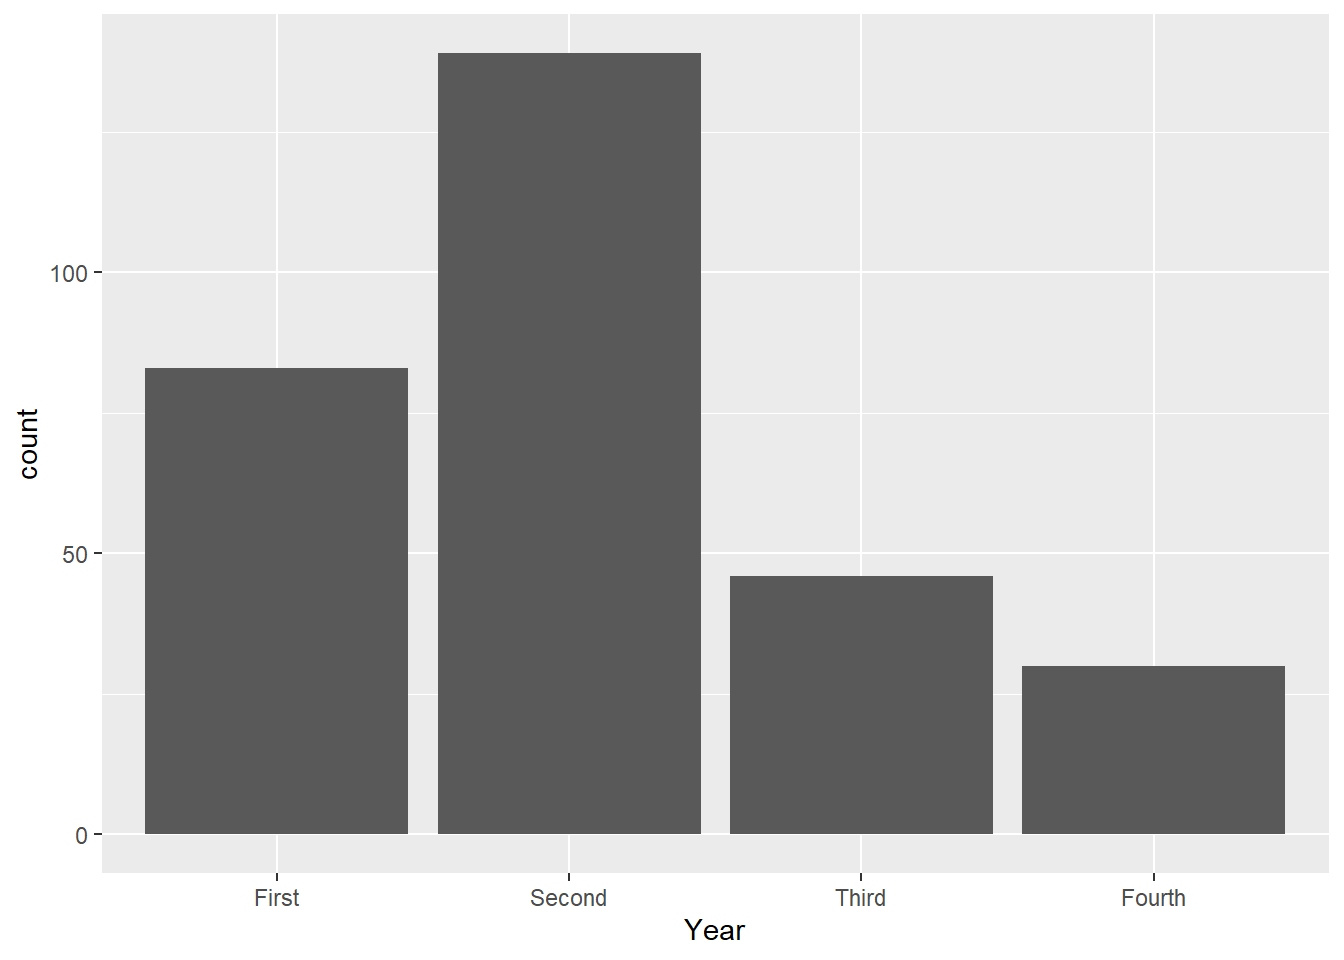
\includegraphics{bookdown-demo_files/figure-latex/unnamed-chunk-69-1.pdf}

We can read the number of students who are first, second, third, and fourth years by reading off the corresponding value on the vertical axis.

From these two lines we code, we can see the basic structure of creating data visualizations with the \texttt{ggplot()} function:

\begin{enumerate}
\def\labelenumi{\arabic{enumi}.}
\item
  Use the \texttt{ggplot()} function, and supply the name of the data frame, and the x- and/or y- variables via the aes() function. End this line with a \texttt{+} operator, and then press enter.
\item
  In the next line, specify the type of graph we want to create (called \texttt{geoms}). For a bar chart, type \texttt{geom\_bar()}.
\end{enumerate}

Some describe these lines of code as two layers of code. These two layers must be supplied for all data visualizations with \texttt{ggplot()}.

Additional optional layers can be added (these usually deal with the details of the visuals). Suppose we want to change the orientation of this bar chart, we can add an optional line, or layer:

\begin{Shaded}
\begin{Highlighting}[]
\FunctionTok{ggplot}\NormalTok{(Data, }\FunctionTok{aes}\NormalTok{(}\AttributeTok{x=}\NormalTok{Year))}\SpecialCharTok{+}
  \FunctionTok{geom\_bar}\NormalTok{()}\SpecialCharTok{+}
  \FunctionTok{coord\_flip}\NormalTok{()}
\end{Highlighting}
\end{Shaded}

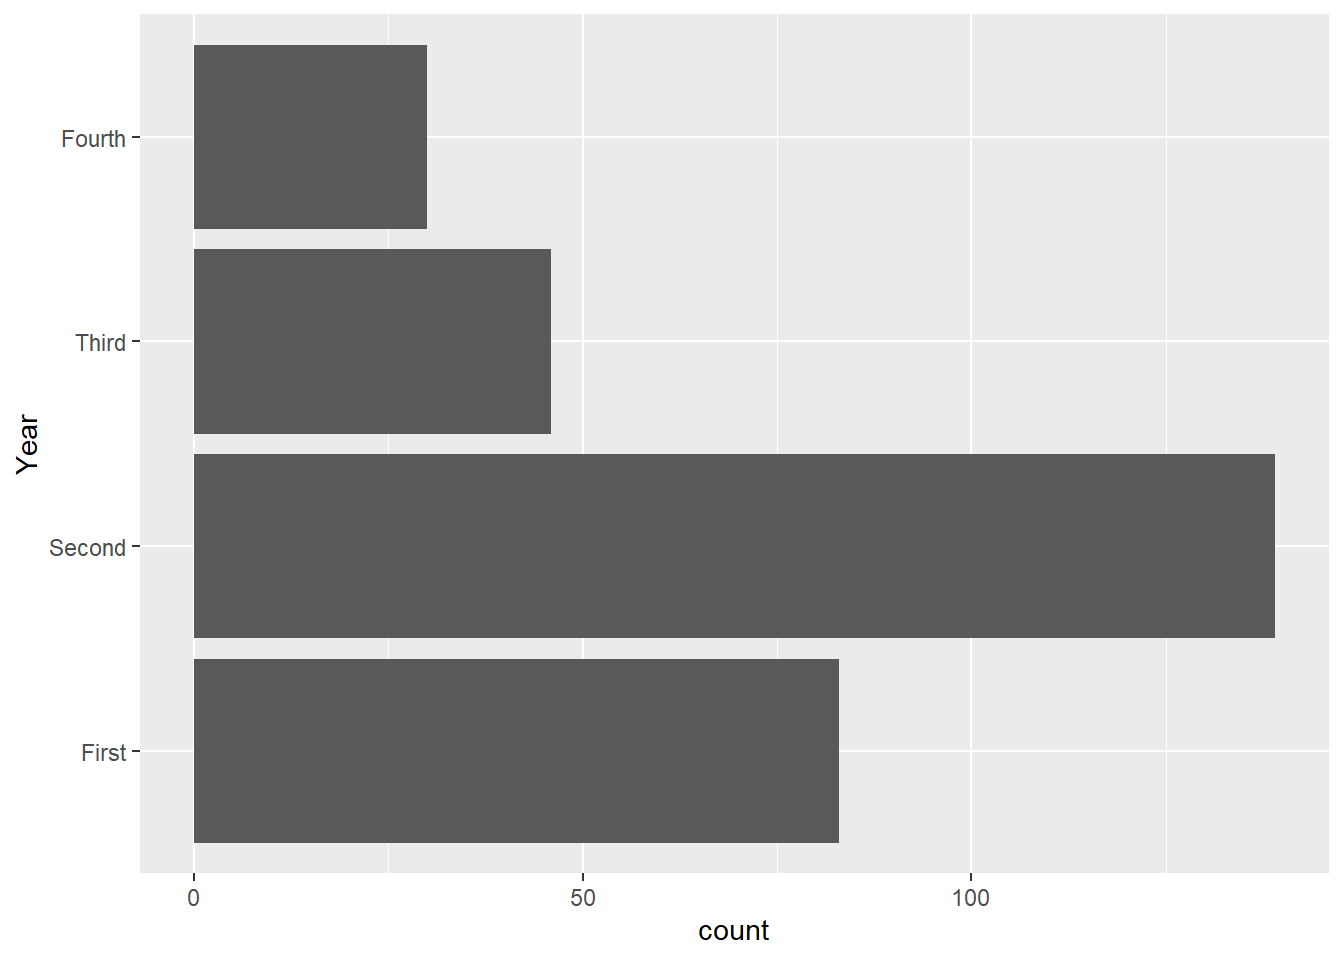
\includegraphics{bookdown-demo_files/figure-latex/unnamed-chunk-70-1.pdf}

It is recommended that each layer is typed on a line below the previous layer. A \texttt{+} sign is used at the end of each layer to add another layer below.

To change the color of the bars:

\begin{Shaded}
\begin{Highlighting}[]
\FunctionTok{ggplot}\NormalTok{(Data, }\FunctionTok{aes}\NormalTok{(}\AttributeTok{x=}\NormalTok{Year))}\SpecialCharTok{+}
  \FunctionTok{geom\_bar}\NormalTok{(}\AttributeTok{fill=}\StringTok{"blue"}\NormalTok{)}
\end{Highlighting}
\end{Shaded}

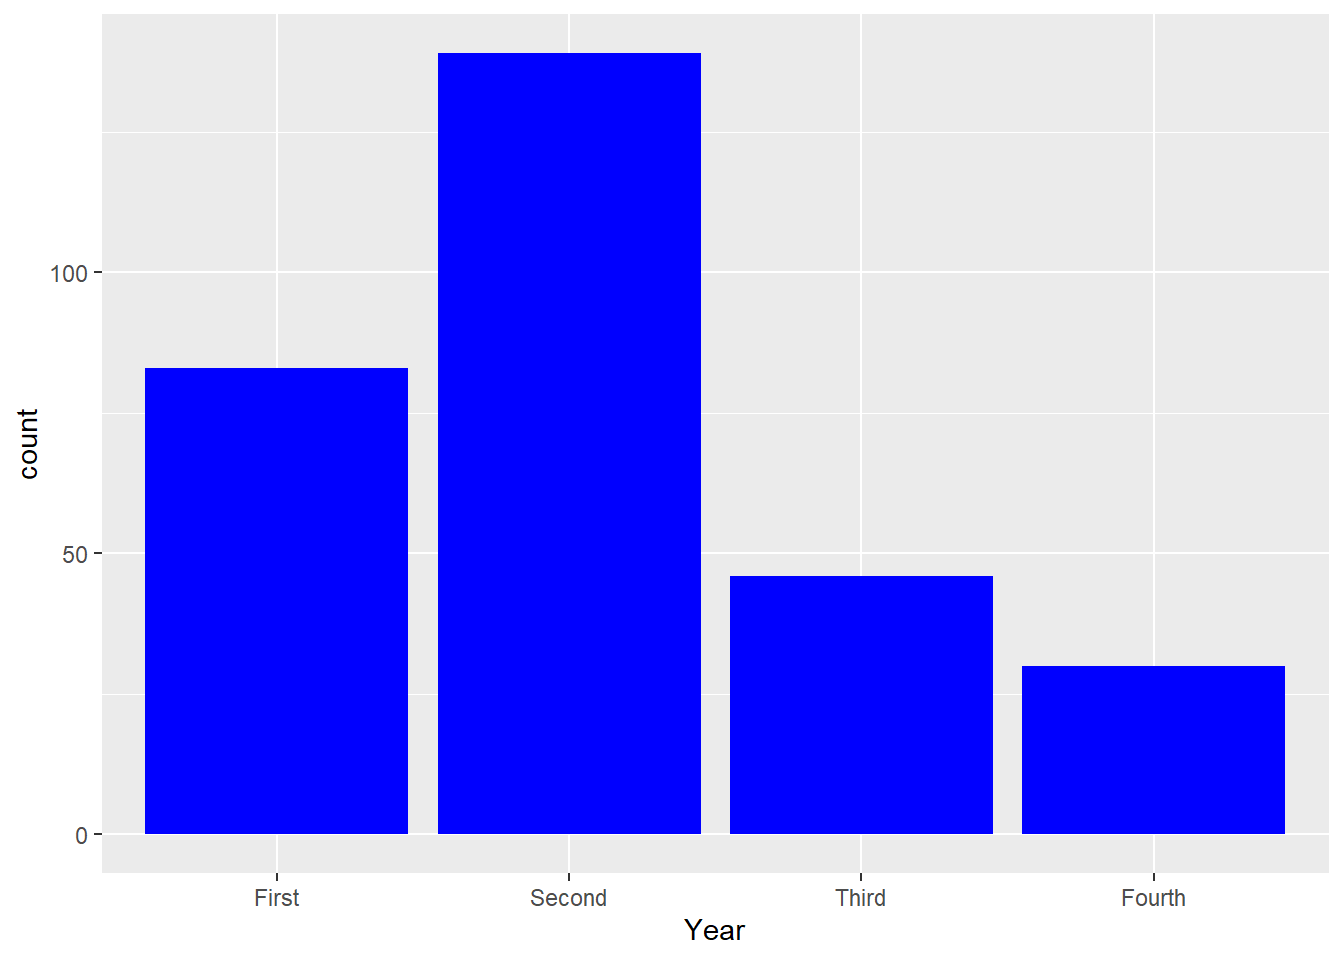
\includegraphics{bookdown-demo_files/figure-latex/unnamed-chunk-71-1.pdf}

To have a different color to outline the bars:

\begin{Shaded}
\begin{Highlighting}[]
\FunctionTok{ggplot}\NormalTok{(Data, }\FunctionTok{aes}\NormalTok{(}\AttributeTok{x=}\NormalTok{Year))}\SpecialCharTok{+}
  \FunctionTok{geom\_bar}\NormalTok{(}\AttributeTok{fill=}\StringTok{"blue"}\NormalTok{,}\AttributeTok{color=}\StringTok{"orange"}\NormalTok{)}
\end{Highlighting}
\end{Shaded}

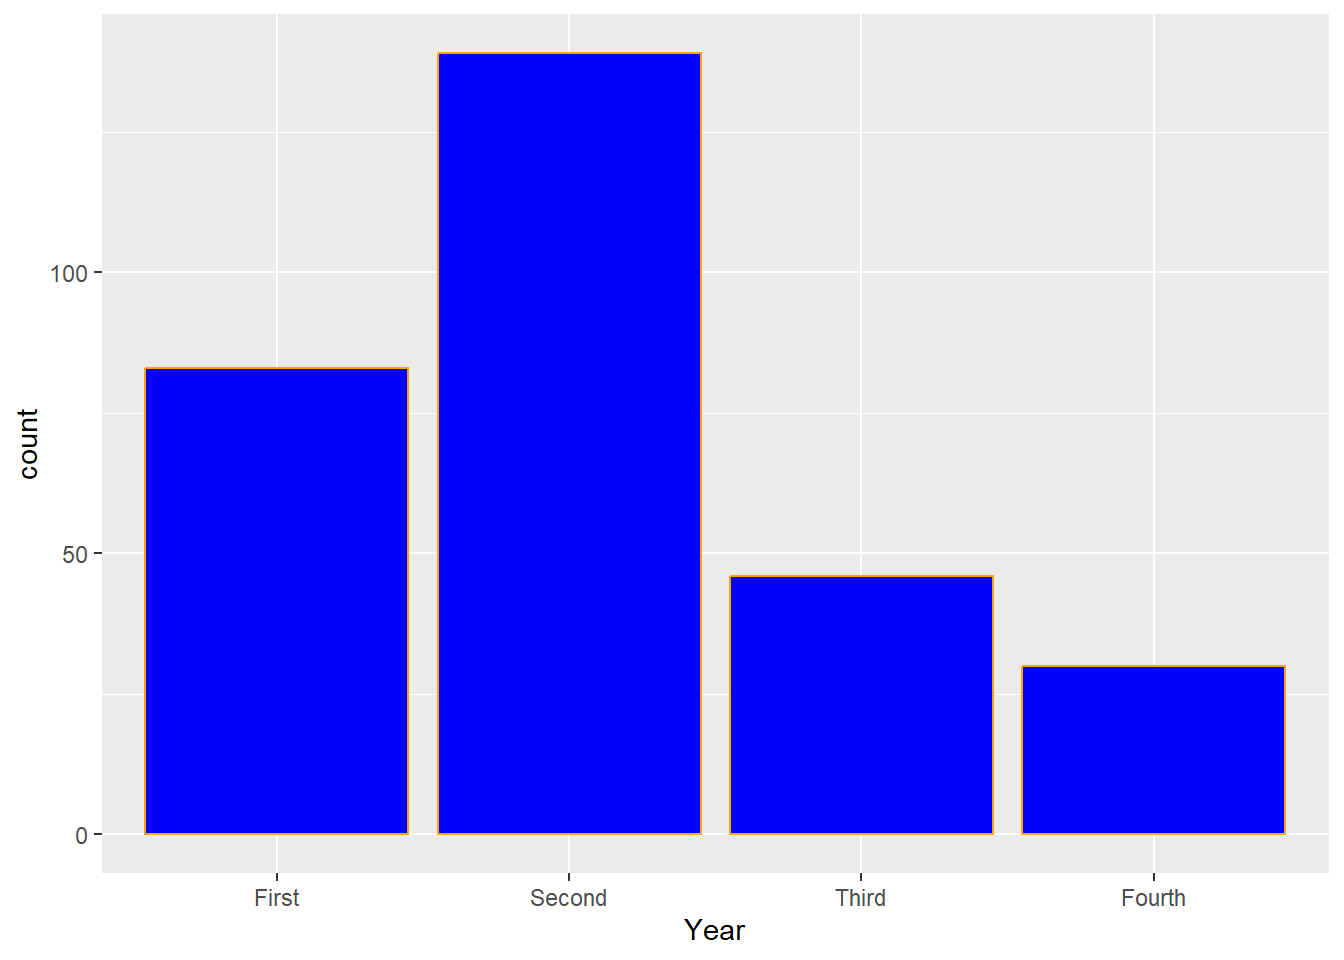
\includegraphics{bookdown-demo_files/figure-latex/unnamed-chunk-72-1.pdf}

\hypertarget{customize-title-and-labels-of-axes-in-bar-charts}{%
\subsubsection{Customize title and labels of axes in bar charts}\label{customize-title-and-labels-of-axes-in-bar-charts}}

To change the orientation of the labels on the horizontal axis, we add an extra layer called \texttt{theme}. This will be useful when we have many classes and/or labels with long names.

To rotate the labels on the horizontal by 90 degrees:

\begin{Shaded}
\begin{Highlighting}[]
\FunctionTok{ggplot}\NormalTok{(Data, }\FunctionTok{aes}\NormalTok{(}\AttributeTok{x=}\NormalTok{Year))}\SpecialCharTok{+}
  \FunctionTok{geom\_bar}\NormalTok{()}\SpecialCharTok{+}
  \FunctionTok{theme}\NormalTok{(}\AttributeTok{axis.text.x =} \FunctionTok{element\_text}\NormalTok{(}\AttributeTok{angle =} \DecValTok{90}\NormalTok{))}
\end{Highlighting}
\end{Shaded}

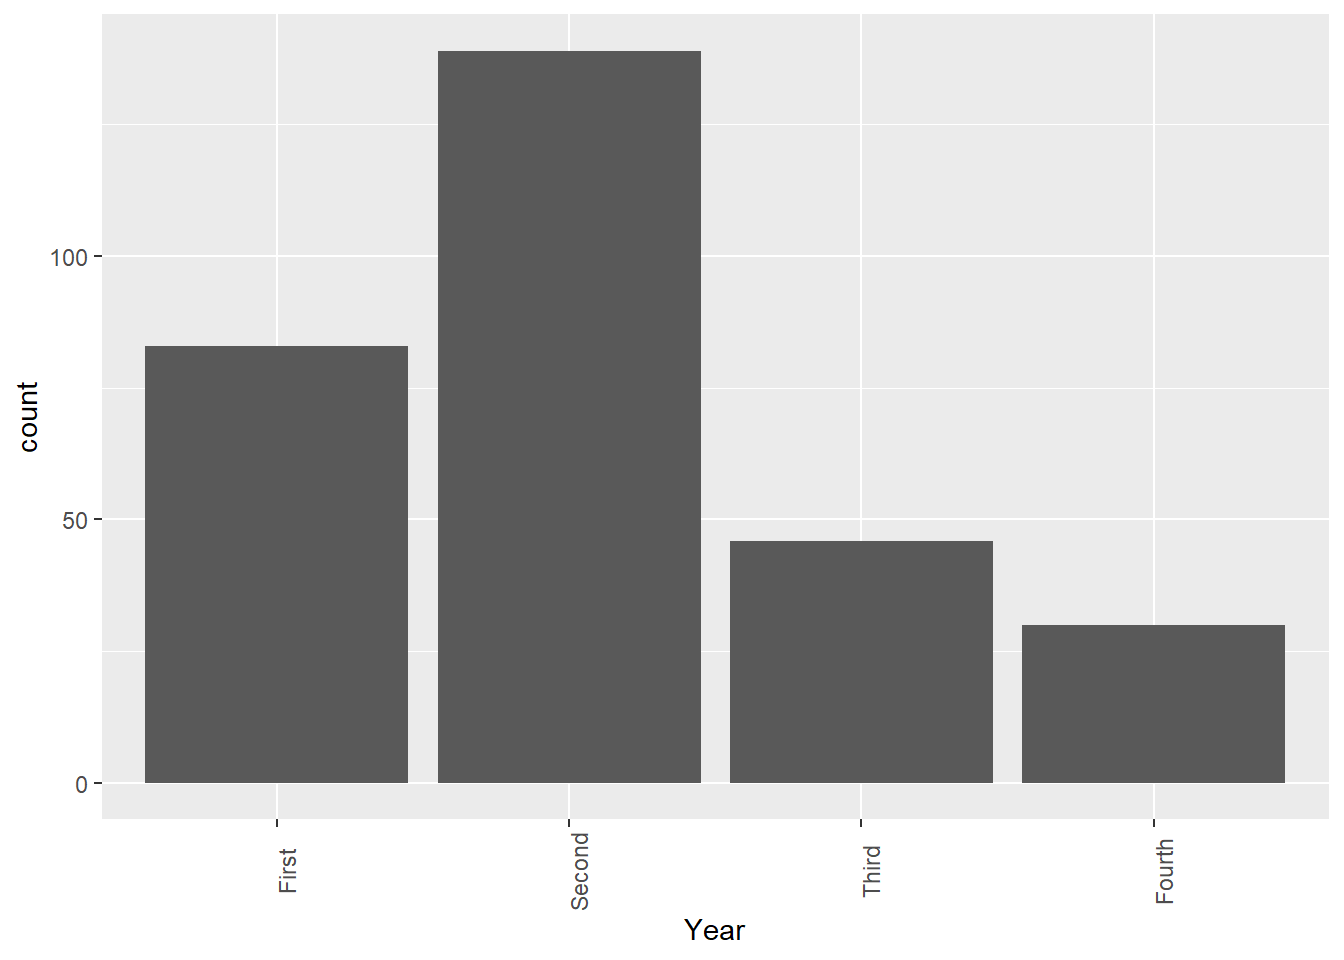
\includegraphics{bookdown-demo_files/figure-latex/unnamed-chunk-73-1.pdf}

As we create more visualizations, it is good practice to give short but meaningful and descriptive names for each axis and provide a title. We can change the labels of the x- and y- axes, as well as add a title for the bar chart by adding another layer called \texttt{labs}:

\begin{Shaded}
\begin{Highlighting}[]
\FunctionTok{ggplot}\NormalTok{(Data, }\FunctionTok{aes}\NormalTok{(}\AttributeTok{x=}\NormalTok{Year))}\SpecialCharTok{+}
  \FunctionTok{geom\_bar}\NormalTok{()}\SpecialCharTok{+}
  \FunctionTok{theme}\NormalTok{(}\AttributeTok{axis.text.x =} \FunctionTok{element\_text}\NormalTok{(}\AttributeTok{angle =} \DecValTok{90}\NormalTok{))}\SpecialCharTok{+}
  \FunctionTok{labs}\NormalTok{(}\AttributeTok{x=}\StringTok{"Year"}\NormalTok{, }\AttributeTok{y=}\StringTok{"Number of Students"}\NormalTok{, }\AttributeTok{title=}\StringTok{"Dist of Years"}\NormalTok{)}
\end{Highlighting}
\end{Shaded}

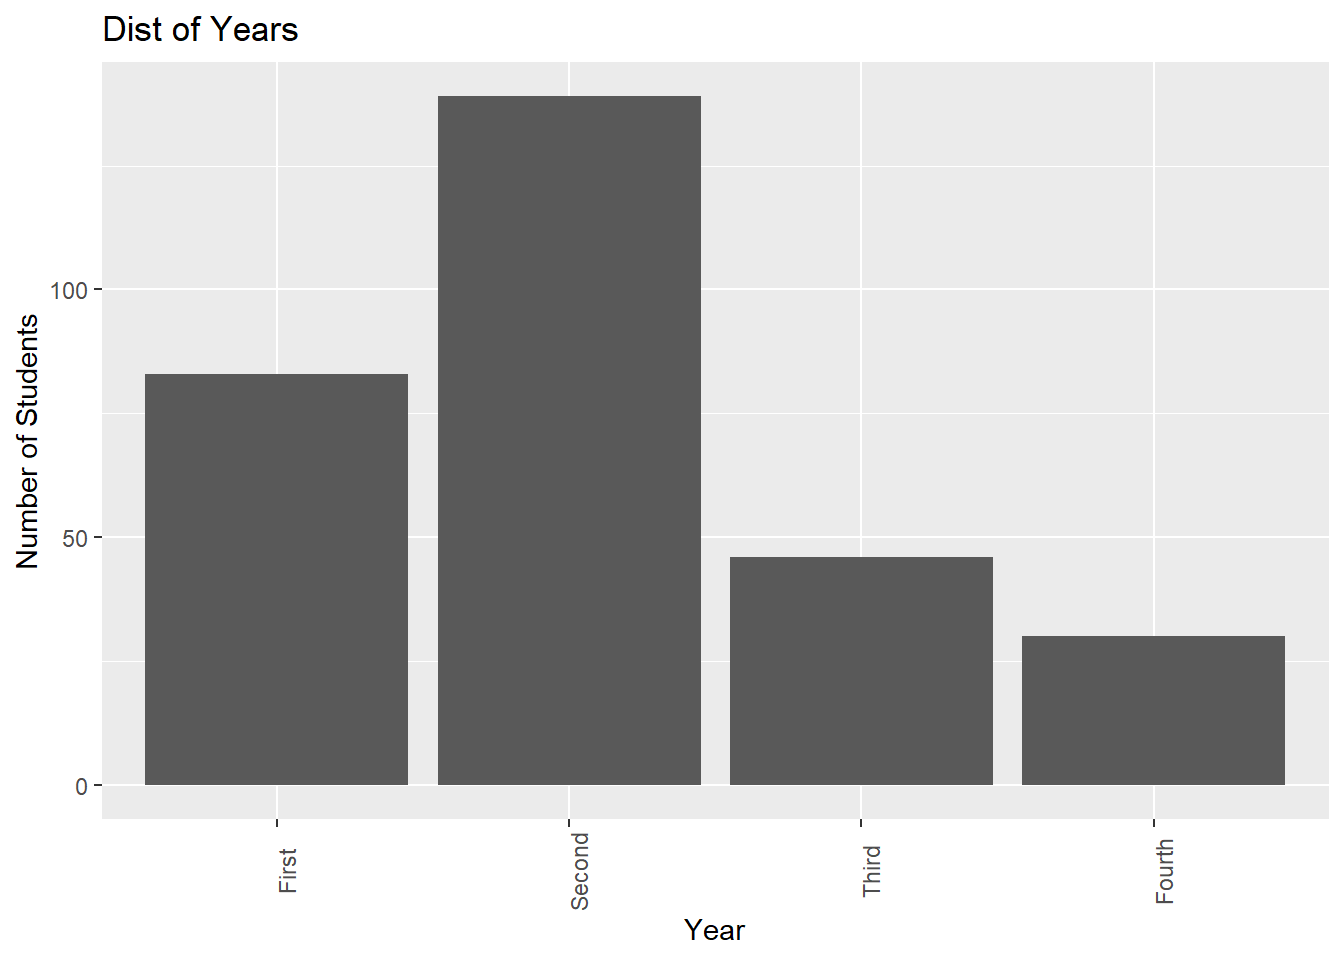
\includegraphics{bookdown-demo_files/figure-latex/unnamed-chunk-74-1.pdf}

We can also adjust the position of the title, for example, center-justify it via \texttt{theme}:

\begin{Shaded}
\begin{Highlighting}[]
\FunctionTok{ggplot}\NormalTok{(Data, }\FunctionTok{aes}\NormalTok{(}\AttributeTok{x=}\NormalTok{Year))}\SpecialCharTok{+}
  \FunctionTok{geom\_bar}\NormalTok{()}\SpecialCharTok{+}
  \FunctionTok{theme}\NormalTok{(}\AttributeTok{axis.text.x =} \FunctionTok{element\_text}\NormalTok{(}\AttributeTok{angle =} \DecValTok{90}\NormalTok{), }
        \AttributeTok{plot.title =} \FunctionTok{element\_text}\NormalTok{(}\AttributeTok{hjust =} \FloatTok{0.5}\NormalTok{))}\SpecialCharTok{+}
  \FunctionTok{labs}\NormalTok{(}\AttributeTok{x=}\StringTok{"Year"}\NormalTok{, }\AttributeTok{y=}\StringTok{"Number of Students"}\NormalTok{, }\AttributeTok{title=}\StringTok{"Dist of Years"}\NormalTok{)}
\end{Highlighting}
\end{Shaded}

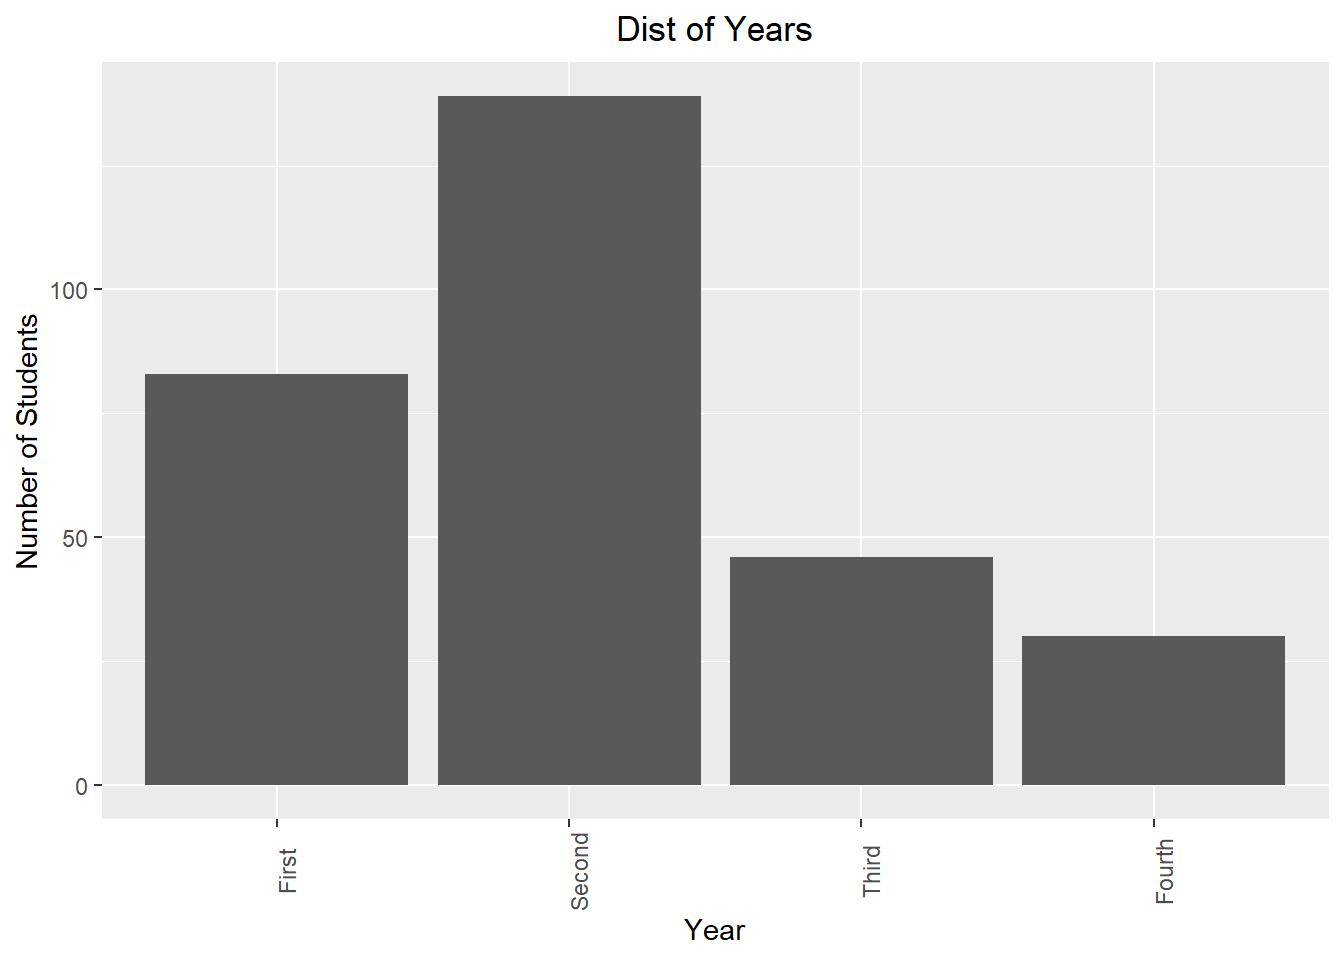
\includegraphics{bookdown-demo_files/figure-latex/unnamed-chunk-75-1.pdf}

\hypertarget{create-a-bar-chart-using-proportions}{%
\subsubsection{Create a bar chart using proportions}\label{create-a-bar-chart-using-proportions}}

Suppose we want to create a bar chart where the y-axis displays the proportions, rather than the counts of each level. There are a few steps to produce such a bar chart. First, we create a new dataframe, where each row represents a year, and we add the proportion of each year into a new column:

\begin{Shaded}
\begin{Highlighting}[]
\NormalTok{newData}\OtherTok{\textless{}{-}}\NormalTok{Data}\SpecialCharTok{\%\textgreater{}\%}
  \FunctionTok{group\_by}\NormalTok{(Year)}\SpecialCharTok{\%\textgreater{}\%}
  \FunctionTok{summarize}\NormalTok{(}\AttributeTok{Counts=}\FunctionTok{n}\NormalTok{())}\SpecialCharTok{\%\textgreater{}\%}
  \FunctionTok{mutate}\NormalTok{(}\AttributeTok{Percent=}\NormalTok{Counts}\SpecialCharTok{/}\FunctionTok{nrow}\NormalTok{(Data))}
\end{Highlighting}
\end{Shaded}

The code above does the following:

\begin{enumerate}
\def\labelenumi{\arabic{enumi}.}
\tightlist
\item
  Creates a new data frame called \texttt{newData} by taking the data frame called \texttt{Data},
\item
  and then groups the observations by \texttt{Year},
\item
  and then counts the number of observations in each \texttt{Year} and stores these values in a vector called \texttt{Counts},
\item
  and then creates a new vector called \texttt{Percent} by using the mathematical operations as specified in \texttt{mutate()}. \texttt{Percent} is added to \texttt{newData}.
\end{enumerate}

We can take a look at the contents of \texttt{newData}:

\begin{Shaded}
\begin{Highlighting}[]
\NormalTok{newData}
\end{Highlighting}
\end{Shaded}

\begin{verbatim}
## # A tibble: 4 x 3
##   Year   Counts Percent
##   <fct>   <int>   <dbl>
## 1 First      83   0.279
## 2 Second    139   0.466
## 3 Third      46   0.154
## 4 Fourth     30   0.101
\end{verbatim}

To create a bar chart using proportions:

\begin{Shaded}
\begin{Highlighting}[]
\FunctionTok{ggplot}\NormalTok{(newData, }\FunctionTok{aes}\NormalTok{(}\AttributeTok{x=}\NormalTok{Year, }\AttributeTok{y=}\NormalTok{Percent))}\SpecialCharTok{+}
  \FunctionTok{geom\_bar}\NormalTok{(}\AttributeTok{stat=}\StringTok{"identity"}\NormalTok{)}\SpecialCharTok{+}
  \FunctionTok{theme}\NormalTok{(}\AttributeTok{axis.text.x =} \FunctionTok{element\_text}\NormalTok{(}\AttributeTok{angle =} \DecValTok{90}\NormalTok{), }
        \AttributeTok{plot.title =} \FunctionTok{element\_text}\NormalTok{(}\AttributeTok{hjust =} \FloatTok{0.5}\NormalTok{))}\SpecialCharTok{+}
  \FunctionTok{labs}\NormalTok{(}\AttributeTok{x=}\StringTok{"Year"}\NormalTok{, }\AttributeTok{y=}\StringTok{"Percent of Students"}\NormalTok{, }\AttributeTok{title=}\StringTok{"Dist of Years"}\NormalTok{)}
\end{Highlighting}
\end{Shaded}

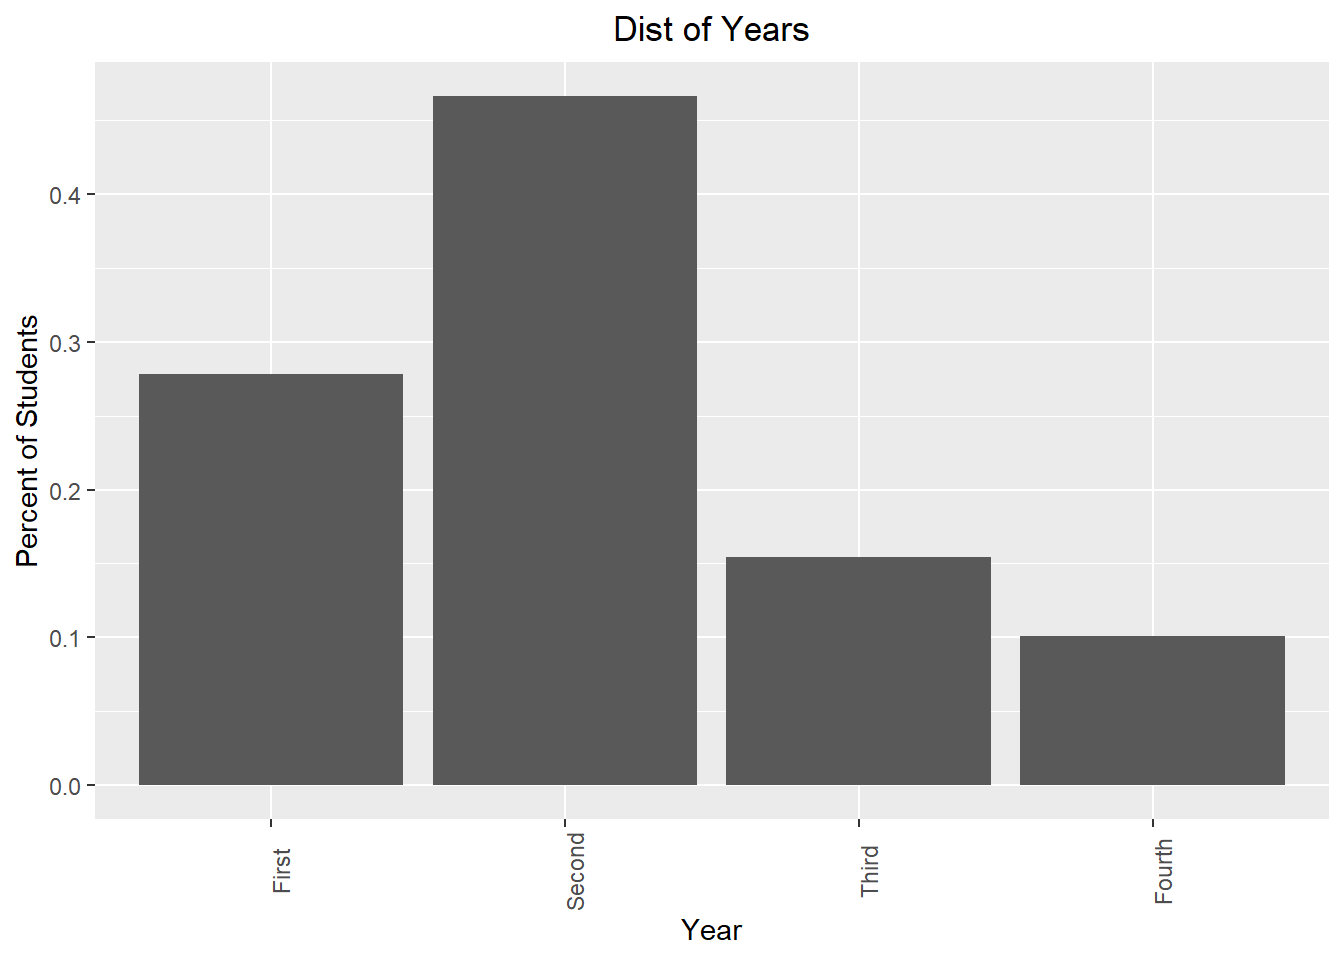
\includegraphics{bookdown-demo_files/figure-latex/unnamed-chunk-78-1.pdf}

Note the following:

\begin{enumerate}
\def\labelenumi{\arabic{enumi}.}
\tightlist
\item
  In the first layer, we use \texttt{newData} instead of the old data frame. In \texttt{aes()}, we specified a y-variable, which we want to be \texttt{Percent}.
\item
  In the second layer, we specified \texttt{stat="identity"} inside \texttt{geom\_bar()}.
\end{enumerate}

\hypertarget{visualizations-with-a-single-quantitative-variable}{%
\section{Visualizations with a Single Quantitative Variable}\label{visualizations-with-a-single-quantitative-variable}}

\hypertarget{number-summary}{%
\subsection{5 number summary}\label{number-summary}}

The \texttt{summary()} function, when applied to a quantitative variable, produces the 5 number summary: the minimum, the first quartile (25th percentile), the median (50th percentile), the third quartile (75th percentile), and the maximum, as well as the mean. For example, to obtain the 5 number summary of the ages of these students:

\begin{Shaded}
\begin{Highlighting}[]
\FunctionTok{summary}\NormalTok{(Data}\SpecialCharTok{$}\NormalTok{Age)}
\end{Highlighting}
\end{Shaded}

\begin{verbatim}
##    Min. 1st Qu.  Median    Mean 3rd Qu.    Max. 
##   18.00   19.00   19.00   19.57   20.00   51.00
\end{verbatim}

The average age of the observations in this dataset is 19.57 years old. Notice the first quartile and the median are both 19 years old, that means at least a quarter of the observations are 19 years old. Also note the maximum of 51 years old, so we have a student who is quite a lot older than the rest.

\hypertarget{boxplots}{%
\subsection{Boxplots}\label{boxplots}}

A boxplot is a graphical representation of the 5 number summary. To create a generic boxplot, we have the following two lines of code when using the \texttt{ggplot()} function:

\begin{Shaded}
\begin{Highlighting}[]
\FunctionTok{ggplot}\NormalTok{(Data, }\FunctionTok{aes}\NormalTok{(}\AttributeTok{y=}\NormalTok{Age))}\SpecialCharTok{+}
  \FunctionTok{geom\_boxplot}\NormalTok{()}
\end{Highlighting}
\end{Shaded}

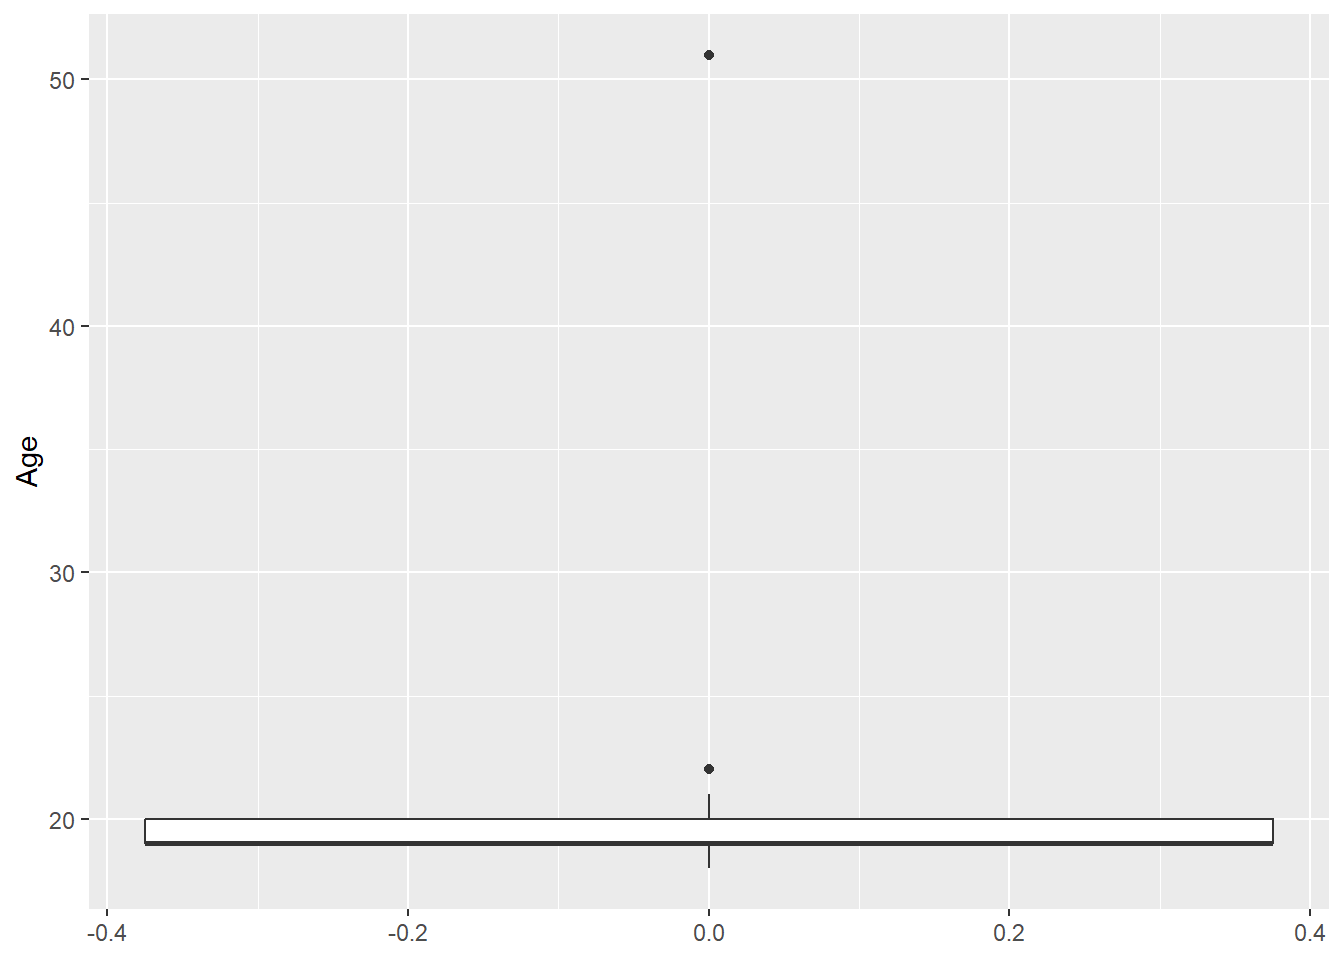
\includegraphics{bookdown-demo_files/figure-latex/unnamed-chunk-80-1.pdf}

Note we are still using the same structure when creating data visualizations with \texttt{ggplot()}:

\begin{enumerate}
\def\labelenumi{\arabic{enumi}.}
\item
  Use the \texttt{ggplot()} function, and supply the name of the data frame, and the x- and/or y- variables via the aes() function. End this line with a \texttt{+} operator, and then press enter.
\item
  In the next line, specify the type of graph we want to create (called \texttt{geoms}). For a boxplot, type \texttt{geom\_boxplot}.
\end{enumerate}

Notice there are outliers (observations that are a lot older or younger) that are denoted by the dots. One is the 51 year old, and 22 year olds are deemed to be outliers. The rule being used is the \(1.5 \times IQR\) rule.

Similar to bar charts, we can change the orientation of boxplots by adding an additional layer as before:

\begin{Shaded}
\begin{Highlighting}[]
\FunctionTok{ggplot}\NormalTok{(Data, }\FunctionTok{aes}\NormalTok{(}\AttributeTok{y=}\NormalTok{Age))}\SpecialCharTok{+}
  \FunctionTok{geom\_boxplot}\NormalTok{()}\SpecialCharTok{+}
  \FunctionTok{coord\_flip}\NormalTok{()}
\end{Highlighting}
\end{Shaded}

We can change the color of the box and the outliers similarly:

\begin{Shaded}
\begin{Highlighting}[]
\FunctionTok{ggplot}\NormalTok{(Data, }\FunctionTok{aes}\NormalTok{(}\AttributeTok{y=}\NormalTok{Age))}\SpecialCharTok{+}
  \FunctionTok{geom\_boxplot}\NormalTok{(}\AttributeTok{color=}\StringTok{"blue"}\NormalTok{, }\AttributeTok{outlier.color =} \StringTok{"orange"}\NormalTok{ )}
\end{Highlighting}
\end{Shaded}

\hypertarget{histograms}{%
\subsection{Histograms}\label{histograms}}

A histogram displays the number of observations within each bin on the x-axis:

\begin{Shaded}
\begin{Highlighting}[]
\FunctionTok{ggplot}\NormalTok{(Data,}\FunctionTok{aes}\NormalTok{(}\AttributeTok{x=}\NormalTok{Age))}\SpecialCharTok{+}
  \FunctionTok{geom\_histogram}\NormalTok{()}
\end{Highlighting}
\end{Shaded}

\begin{verbatim}
## `stat_bin()` using `bins = 30`. Pick better value with `binwidth`.
\end{verbatim}

Notice a warning message is displayed when creating a basic histogram. To fix this, we use the binwidth argument within \texttt{geom\_histogram}. We try \texttt{binwidth=1} for now, which means the width of the bin is 1 unit:

\begin{Shaded}
\begin{Highlighting}[]
\FunctionTok{ggplot}\NormalTok{(Data,}\FunctionTok{aes}\NormalTok{(}\AttributeTok{x=}\NormalTok{Age))}\SpecialCharTok{+}
  \FunctionTok{geom\_histogram}\NormalTok{(}\AttributeTok{binwidth =} \DecValTok{1}\NormalTok{,}\AttributeTok{fill=}\StringTok{"blue"}\NormalTok{,}\AttributeTok{color=}\StringTok{"orange"}\NormalTok{)}
\end{Highlighting}
\end{Shaded}

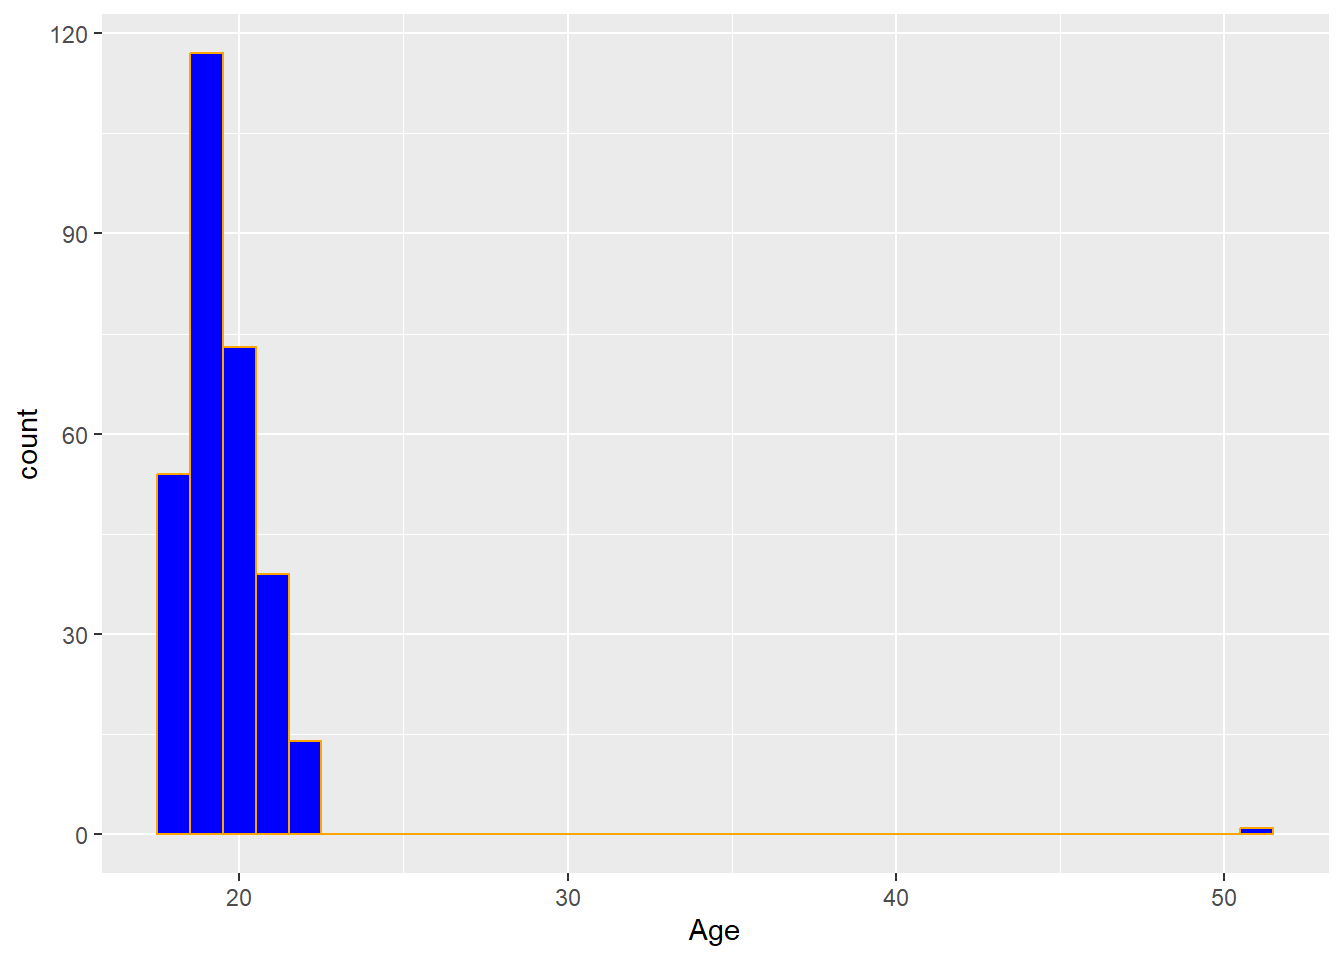
\includegraphics{bookdown-demo_files/figure-latex/unnamed-chunk-84-1.pdf}

The ages of the students are mostly young, with 19 and 20 years olds being the most commonly occuring.

A well-known drawback of histograms is that the width of the bins can drastically affect the visual. For example, suppose we change the binwidth to 2:

\begin{Shaded}
\begin{Highlighting}[]
\FunctionTok{ggplot}\NormalTok{(Data,}\FunctionTok{aes}\NormalTok{(}\AttributeTok{x=}\NormalTok{Age))}\SpecialCharTok{+}
  \FunctionTok{geom\_histogram}\NormalTok{(}\AttributeTok{binwidth =} \DecValTok{2}\NormalTok{,}\AttributeTok{fill=}\StringTok{"blue"}\NormalTok{,}\AttributeTok{color=}\StringTok{"orange"}\NormalTok{)}
\end{Highlighting}
\end{Shaded}

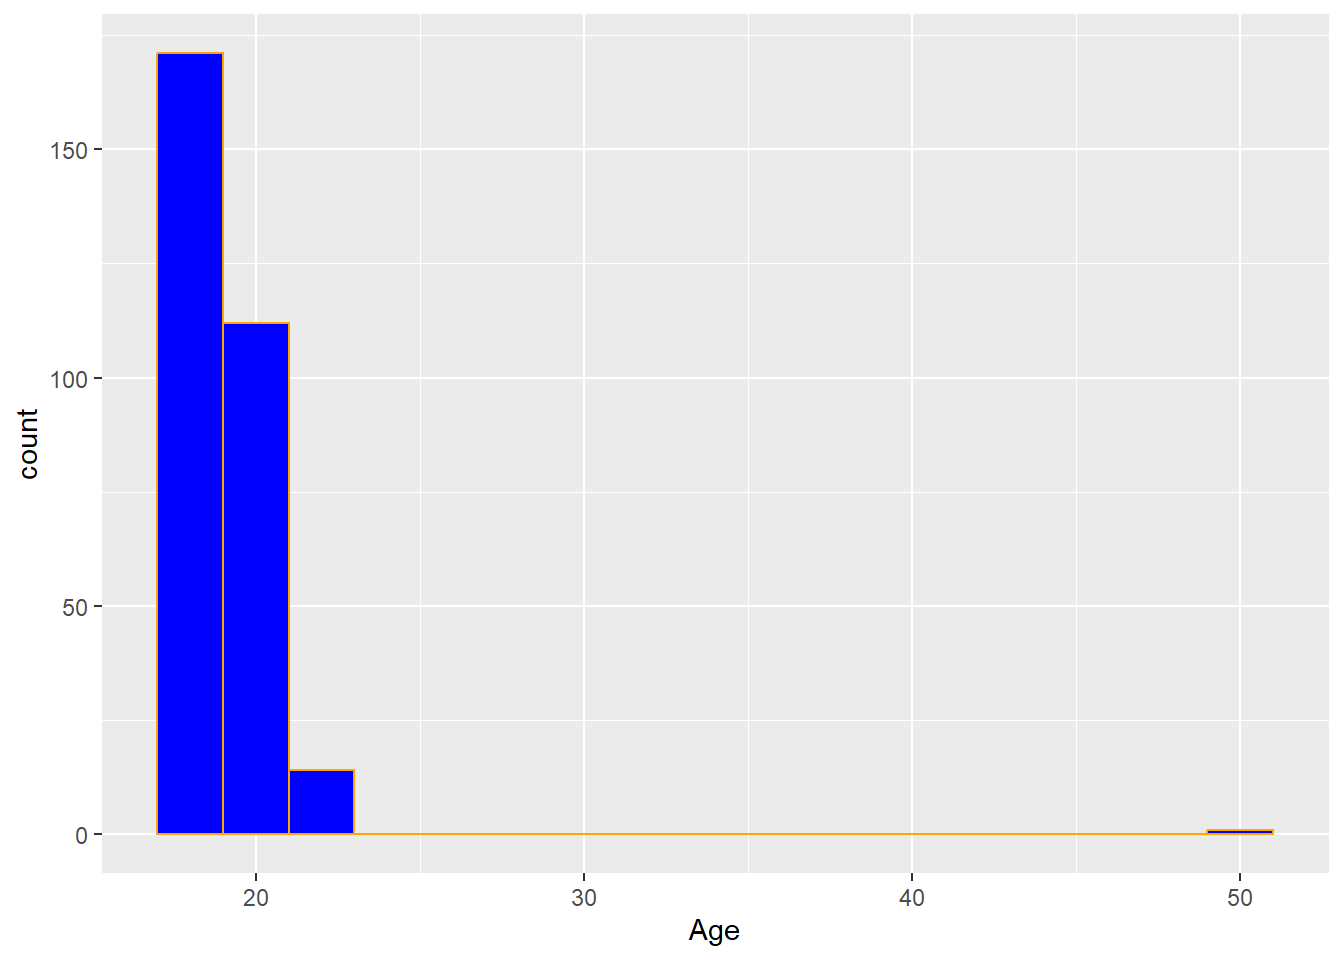
\includegraphics{bookdown-demo_files/figure-latex/unnamed-chunk-85-1.pdf}

Each bar now contains two ages: the first bar contains the 18 and 19 year olds. Notice how the shape has been changed a little bit from the previous histogram with a different binwidth?

\hypertarget{density-plots}{%
\subsection{Density plots}\label{density-plots}}

Density plots are a variation of histograms, where the plot attempts to use a smooth mathematical function to approximate the shape of the histogram, and is unaffected by binwidth:

\begin{Shaded}
\begin{Highlighting}[]
\FunctionTok{ggplot}\NormalTok{(Data,}\FunctionTok{aes}\NormalTok{(}\AttributeTok{x=}\NormalTok{Age))}\SpecialCharTok{+}
  \FunctionTok{geom\_density}\NormalTok{()}
\end{Highlighting}
\end{Shaded}

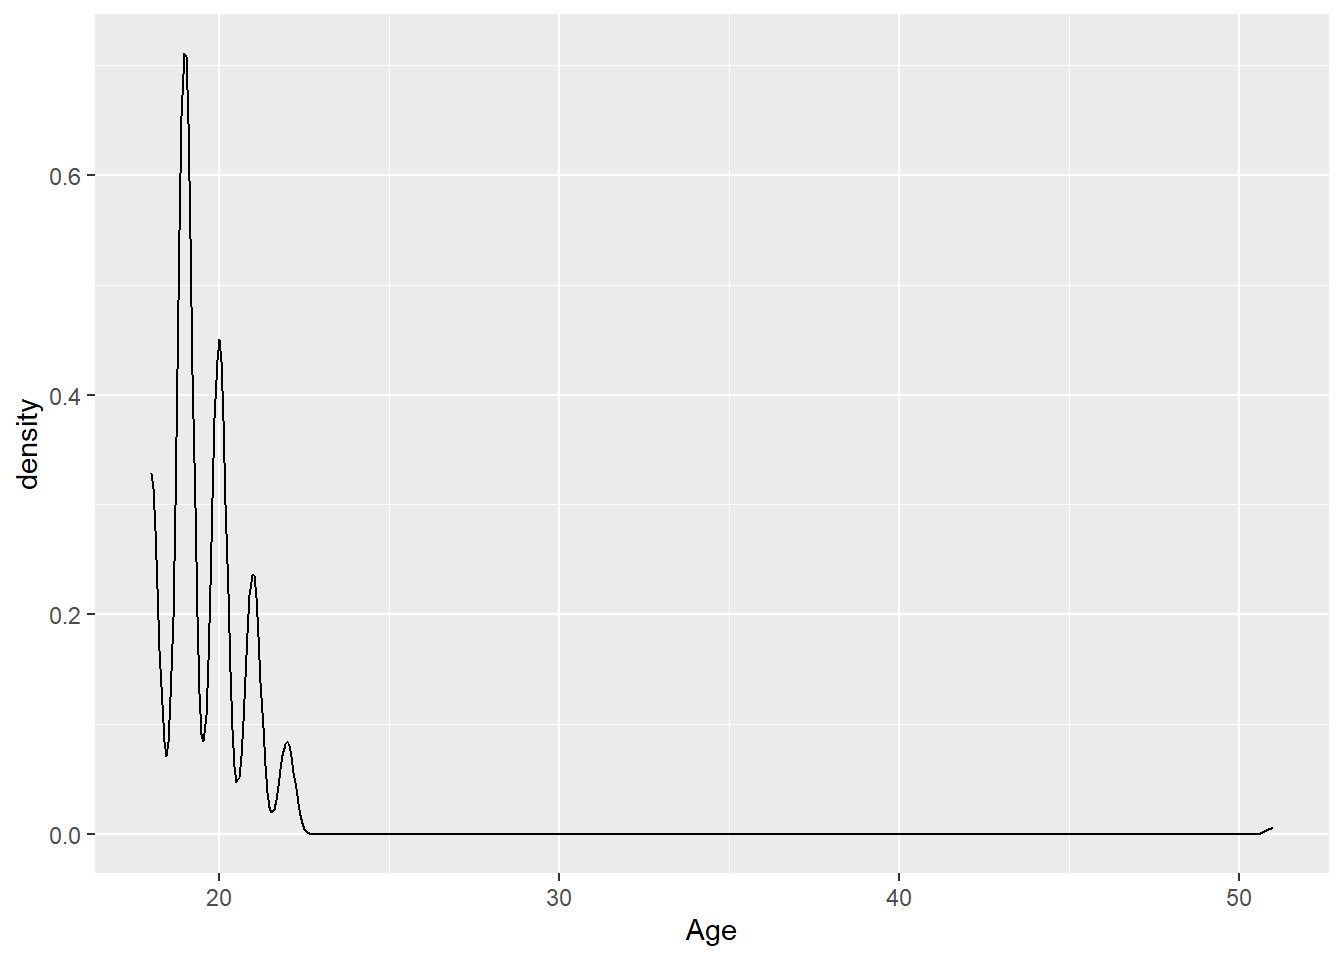
\includegraphics{bookdown-demo_files/figure-latex/unnamed-chunk-86-1.pdf}

We can see that 19 and 20 year olds are the most common ages in this data. Be careful in interpreting the values on the veritical axis: these do not represent proportions. A characteristic of density plots is that the area under the plot is always one.

\hypertarget{bivariate-visualizations}{%
\section{Bivariate Visualizations}\label{bivariate-visualizations}}

We will now look at visualizations we can create to explore the relationship between two variables. The term bivariate means that we are looking at two variables.

We will be using a new dataset as an example, so we clear the environment:

\begin{Shaded}
\begin{Highlighting}[]
\FunctionTok{rm}\NormalTok{(}\AttributeTok{list =} \FunctionTok{ls}\NormalTok{())}
\end{Highlighting}
\end{Shaded}

We will be using the dataset, \texttt{gapminder}, from the \texttt{gapminder} package. Install and load the \texttt{gapminder} package. Also load the \texttt{tidyverse} package (which automatically loads the \texttt{ggplot2} package):

\begin{Shaded}
\begin{Highlighting}[]
\FunctionTok{library}\NormalTok{(tidyverse)}
\FunctionTok{library}\NormalTok{(gapminder)}
\end{Highlighting}
\end{Shaded}

We can take a look at the \texttt{gapminder} dataset:

\begin{Shaded}
\begin{Highlighting}[]
\NormalTok{gapminder[}\DecValTok{1}\SpecialCharTok{:}\DecValTok{15}\NormalTok{,]}
\end{Highlighting}
\end{Shaded}

\begin{verbatim}
## # A tibble: 15 x 6
##    country     continent  year lifeExp      pop gdpPercap
##    <fct>       <fct>     <int>   <dbl>    <int>     <dbl>
##  1 Afghanistan Asia       1952    28.8  8425333      779.
##  2 Afghanistan Asia       1957    30.3  9240934      821.
##  3 Afghanistan Asia       1962    32.0 10267083      853.
##  4 Afghanistan Asia       1967    34.0 11537966      836.
##  5 Afghanistan Asia       1972    36.1 13079460      740.
##  6 Afghanistan Asia       1977    38.4 14880372      786.
##  7 Afghanistan Asia       1982    39.9 12881816      978.
##  8 Afghanistan Asia       1987    40.8 13867957      852.
##  9 Afghanistan Asia       1992    41.7 16317921      649.
## 10 Afghanistan Asia       1997    41.8 22227415      635.
## 11 Afghanistan Asia       2002    42.1 25268405      727.
## 12 Afghanistan Asia       2007    43.8 31889923      975.
## 13 Albania     Europe     1952    55.2  1282697     1601.
## 14 Albania     Europe     1957    59.3  1476505     1942.
## 15 Albania     Europe     1962    64.8  1728137     2313.
\end{verbatim}

Per the documentation, the variables are

\begin{enumerate}
\def\labelenumi{\arabic{enumi}.}
\tightlist
\item
  \texttt{country}
\item
  \texttt{continent}
\item
  \texttt{year}: from 1952 to 2007 in increments of 5 years
\item
  \texttt{lifeExp}: life expectancy at birth, in years
\item
  \texttt{pop}: population of country
\item
  \texttt{gdpPercap}: GDP per capita in US dollars, adjusted for inflation
\end{enumerate}

We notice that data are collected from each country across a number of different years: 1952 to 2007 in increments of five years. For this example, we will mainly focus on the data for the most recent year, 2007:

\begin{Shaded}
\begin{Highlighting}[]
\NormalTok{Data}\OtherTok{\textless{}{-}}\NormalTok{gapminder}\SpecialCharTok{\%\textgreater{}\%}
  \FunctionTok{filter}\NormalTok{(year}\SpecialCharTok{==}\DecValTok{2007}\NormalTok{)}
\end{Highlighting}
\end{Shaded}

The specific visuals to use will again depend on the type of variables we are using, whether they are categorical or quantitative.

\hypertarget{compare-quantitative-variable-across-categories}{%
\subsection{Compare quantitative variable across categories}\label{compare-quantitative-variable-across-categories}}

\hypertarget{side-by-side-boxplots}{%
\subsubsection{Side by side boxplots}\label{side-by-side-boxplots}}

Side by side boxplots are useful to compare a quantitative variable across different classes of a categorical variable. For example, we want to compare life expectancies across the different continents in the year 2007:

\begin{Shaded}
\begin{Highlighting}[]
\FunctionTok{ggplot}\NormalTok{(Data, }\FunctionTok{aes}\NormalTok{(}\AttributeTok{x=}\NormalTok{continent, }\AttributeTok{y=}\NormalTok{lifeExp))}\SpecialCharTok{+}
  \FunctionTok{geom\_boxplot}\NormalTok{(}\AttributeTok{fill=}\StringTok{"Blue"}\NormalTok{)}\SpecialCharTok{+}
  \FunctionTok{labs}\NormalTok{(}\AttributeTok{x=}\StringTok{"Continent"}\NormalTok{, }\AttributeTok{y=}\StringTok{"Life Exp"}\NormalTok{, }\AttributeTok{title=}\StringTok{"Dist of Life Expectancies by Continent"}\NormalTok{)}
\end{Highlighting}
\end{Shaded}

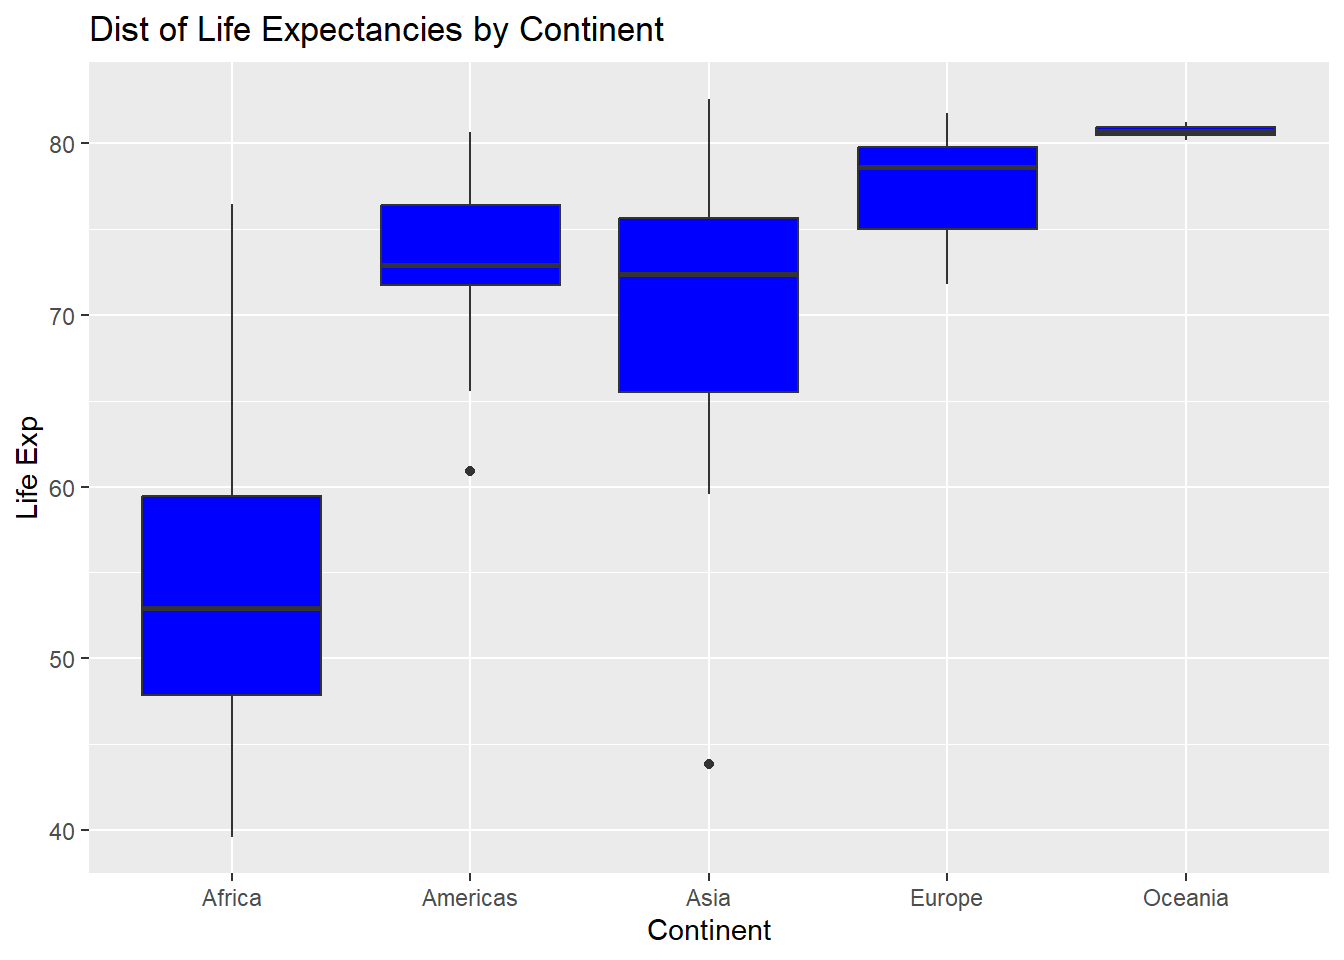
\includegraphics{bookdown-demo_files/figure-latex/unnamed-chunk-91-1.pdf}

Countries in the Oceania region have long life expectancies with little variation. Comparing the Americas and Asia, the median life expectancies are similar, but the spread is larger for Asia.

\hypertarget{violin-plots}{%
\subsubsection{Violin plots}\label{violin-plots}}

Violin plots are an alternative to boxplots. To create these plots to compare life expectancies across the different continents in the year 2007:

\begin{Shaded}
\begin{Highlighting}[]
\FunctionTok{ggplot}\NormalTok{(Data, }\FunctionTok{aes}\NormalTok{(}\AttributeTok{x=}\NormalTok{continent, }\AttributeTok{y=}\NormalTok{lifeExp))}\SpecialCharTok{+}
  \FunctionTok{geom\_violin}\NormalTok{()}\SpecialCharTok{+}
  \FunctionTok{labs}\NormalTok{(}\AttributeTok{x=}\StringTok{"Continent"}\NormalTok{, }\AttributeTok{y=}\StringTok{"Life Exp"}\NormalTok{, }\AttributeTok{title=}\StringTok{"Dist of Life Expectancies by Continent"}\NormalTok{)}
\end{Highlighting}
\end{Shaded}

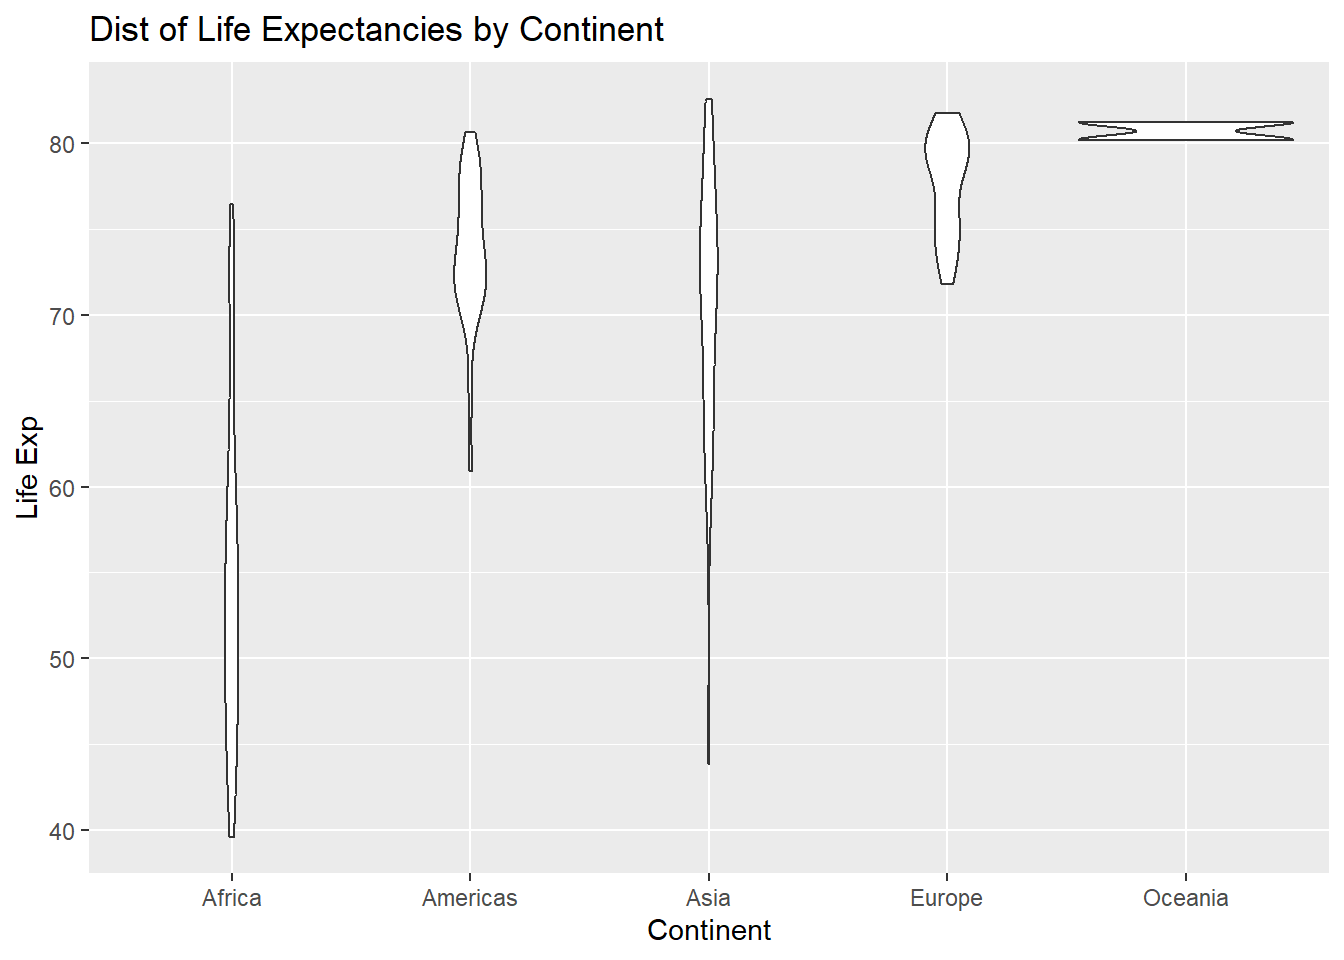
\includegraphics{bookdown-demo_files/figure-latex/unnamed-chunk-92-1.pdf}

The width of the violin informs us which values are more commonly occuring. For example, look at the violin for Europe. The violin is wider at higher life expectancies, so longer life expectancies are more common in European countries.

\hypertarget{summarizing-two-categorical-variables}{%
\subsection{Summarizing two categorical variables}\label{summarizing-two-categorical-variables}}

For this example, we create a new binary variable called \texttt{expectancy}, which will be denoted as \texttt{low} if the life expectancy in the country is less than 70 years, and \texttt{high} otherwise:

\begin{Shaded}
\begin{Highlighting}[]
\NormalTok{Data}\OtherTok{\textless{}{-}}\NormalTok{Data}\SpecialCharTok{\%\textgreater{}\%}
  \FunctionTok{mutate}\NormalTok{(}\AttributeTok{expectancy=}\FunctionTok{ifelse}\NormalTok{(lifeExp}\SpecialCharTok{\textless{}}\DecValTok{70}\NormalTok{,}\StringTok{"Low"}\NormalTok{,}\StringTok{"High"}\NormalTok{))}
\end{Highlighting}
\end{Shaded}

\hypertarget{two-way-tables}{%
\subsubsection{Two-way tables}\label{two-way-tables}}

Suppose we want to see how \texttt{expectancy} varies across the continents. A two-way table can be created for produce counts when two categorical variables are involved:

\begin{Shaded}
\begin{Highlighting}[]
\NormalTok{mytab2}\OtherTok{\textless{}{-}}\FunctionTok{table}\NormalTok{(Data}\SpecialCharTok{$}\NormalTok{continent, Data}\SpecialCharTok{$}\NormalTok{expectancy)}
\DocumentationTok{\#\#continent in rows, expectancy in columns}
\NormalTok{mytab2}
\end{Highlighting}
\end{Shaded}

\begin{verbatim}
##           
##            High Low
##   Africa      7  45
##   Americas   22   3
##   Asia       22  11
##   Europe     30   0
##   Oceania     2   0
\end{verbatim}

The first variable in \texttt{table()} will be placed in the rows, the second variable will be placed in the columns.

From this table, we can see that 22 countries in the Americas have high life expectancies, while 3 countries in the Americas have low life expectancies.

We may be interested in looking at the proportions, instead of counts, of countries in each continent that have high or low life expectancies. To convert this table to proportions, we can use \texttt{prop.table()}:

\begin{Shaded}
\begin{Highlighting}[]
\FunctionTok{prop.table}\NormalTok{(mytab2, }\DecValTok{1}\NormalTok{) }
\end{Highlighting}
\end{Shaded}

\begin{verbatim}
##           
##                 High       Low
##   Africa   0.1346154 0.8653846
##   Americas 0.8800000 0.1200000
##   Asia     0.6666667 0.3333333
##   Europe   1.0000000 0.0000000
##   Oceania  1.0000000 0.0000000
\end{verbatim}

We want proportions for each continent, so we want proportions in each row to add up to 1. Therefore, the second argument in \texttt{prop.table()} is 1. Enter 2 for this argument if we want the proportions in each column to add up to 1.

As before, to convert to percentages and round to 2 decimal places:

\begin{Shaded}
\begin{Highlighting}[]
\FunctionTok{round}\NormalTok{(}\FunctionTok{prop.table}\NormalTok{(mytab2, }\DecValTok{1}\NormalTok{) }\SpecialCharTok{*} \DecValTok{100}\NormalTok{, }\DecValTok{2}\NormalTok{)}
\end{Highlighting}
\end{Shaded}

\begin{verbatim}
##           
##              High    Low
##   Africa    13.46  86.54
##   Americas  88.00  12.00
##   Asia      66.67  33.33
##   Europe   100.00   0.00
##   Oceania  100.00   0.00
\end{verbatim}

\hypertarget{bar-charts-1}{%
\subsubsection{Bar charts}\label{bar-charts-1}}

A stacked bar chart can be used to display the relationship between the binary variable \texttt{expectancy} across continents:

\begin{Shaded}
\begin{Highlighting}[]
\FunctionTok{ggplot}\NormalTok{(Data, }\FunctionTok{aes}\NormalTok{(}\AttributeTok{x=}\NormalTok{continent, }\AttributeTok{fill=}\NormalTok{expectancy))}\SpecialCharTok{+}
  \FunctionTok{geom\_bar}\NormalTok{(}\AttributeTok{position =} \StringTok{"stack"}\NormalTok{)}\SpecialCharTok{+}
  \FunctionTok{labs}\NormalTok{(}\AttributeTok{x=}\StringTok{"Continent"}\NormalTok{, }\AttributeTok{y=}\StringTok{"Count"}\NormalTok{, }\AttributeTok{title=}\StringTok{"Life Expectancies by Continent"}\NormalTok{)}
\end{Highlighting}
\end{Shaded}

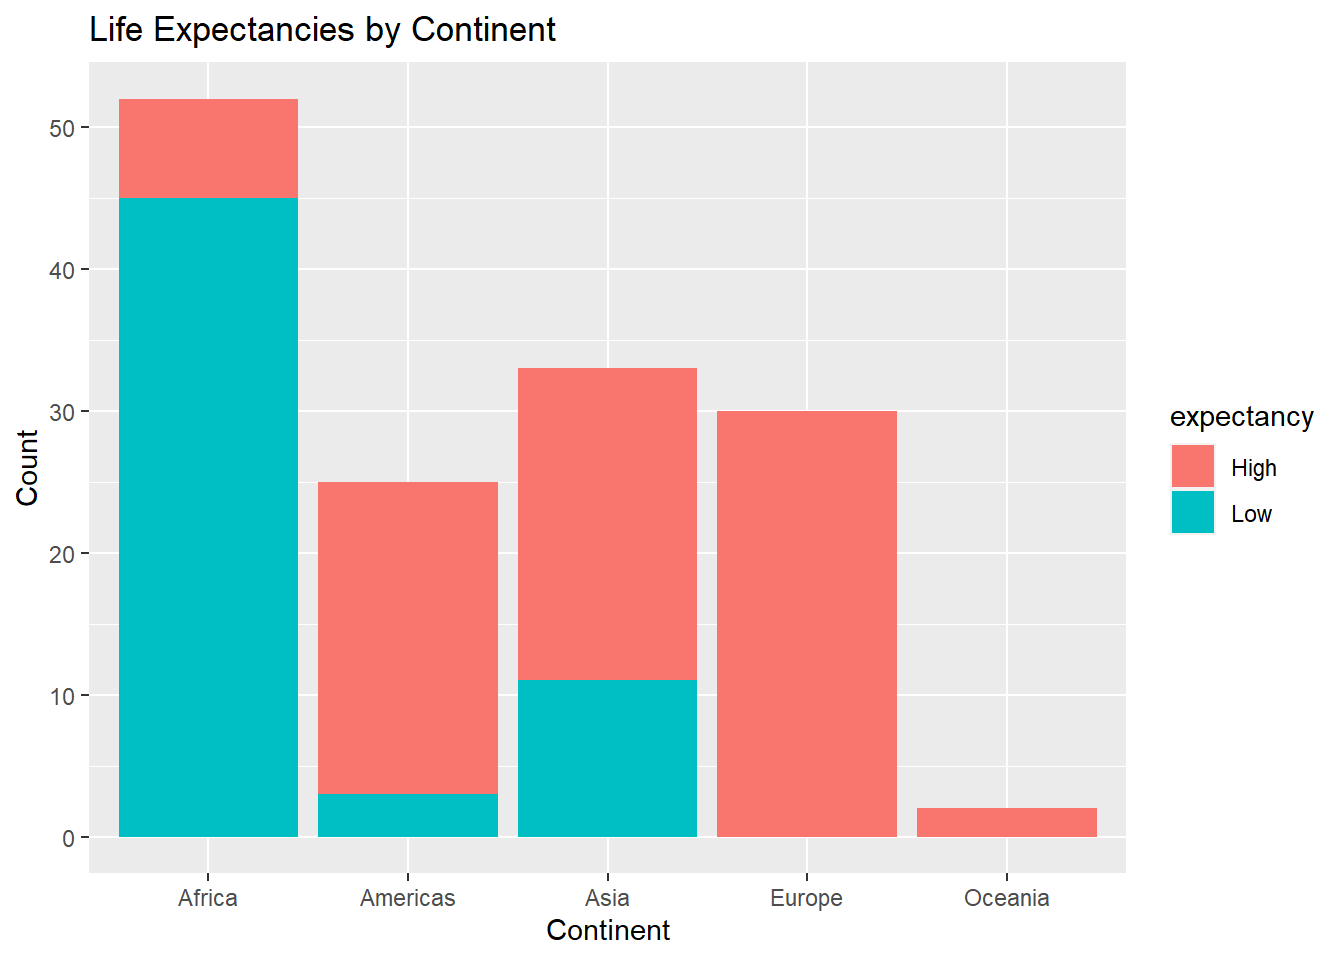
\includegraphics{bookdown-demo_files/figure-latex/unnamed-chunk-97-1.pdf}

We can see how many countries exist in each continent, and how many of these countries in each continent have high or low life expectancies. For example, there are about 25 countries in the Americas with the majority having high life expectancies.

We can change the way the bar chart is displayed by changing \texttt{position} in \texttt{geom\_bar()} to \texttt{position\ =\ "dodge"} or \texttt{position\ =\ "fill"}, the latter being more useful for proportions instead of counts:

\begin{Shaded}
\begin{Highlighting}[]
\FunctionTok{ggplot}\NormalTok{(Data, }\FunctionTok{aes}\NormalTok{(}\AttributeTok{x=}\NormalTok{continent, }\AttributeTok{fill=}\NormalTok{expectancy))}\SpecialCharTok{+}
  \FunctionTok{geom\_bar}\NormalTok{(}\AttributeTok{position =} \StringTok{"dodge"}\NormalTok{) }
\end{Highlighting}
\end{Shaded}

\begin{Shaded}
\begin{Highlighting}[]
\FunctionTok{ggplot}\NormalTok{(Data, }\FunctionTok{aes}\NormalTok{(}\AttributeTok{x=}\NormalTok{continent, }\AttributeTok{fill=}\NormalTok{expectancy))}\SpecialCharTok{+}
  \FunctionTok{geom\_bar}\NormalTok{(}\AttributeTok{position =} \StringTok{"fill"}\NormalTok{)}\SpecialCharTok{+}
  \FunctionTok{labs}\NormalTok{(}\AttributeTok{x=}\StringTok{"Continent"}\NormalTok{, }\AttributeTok{y=}\StringTok{"Proportion"}\NormalTok{, }
       \AttributeTok{title=}\StringTok{"Proportion of Life Expectancies by Continent"}\NormalTok{)}
\end{Highlighting}
\end{Shaded}

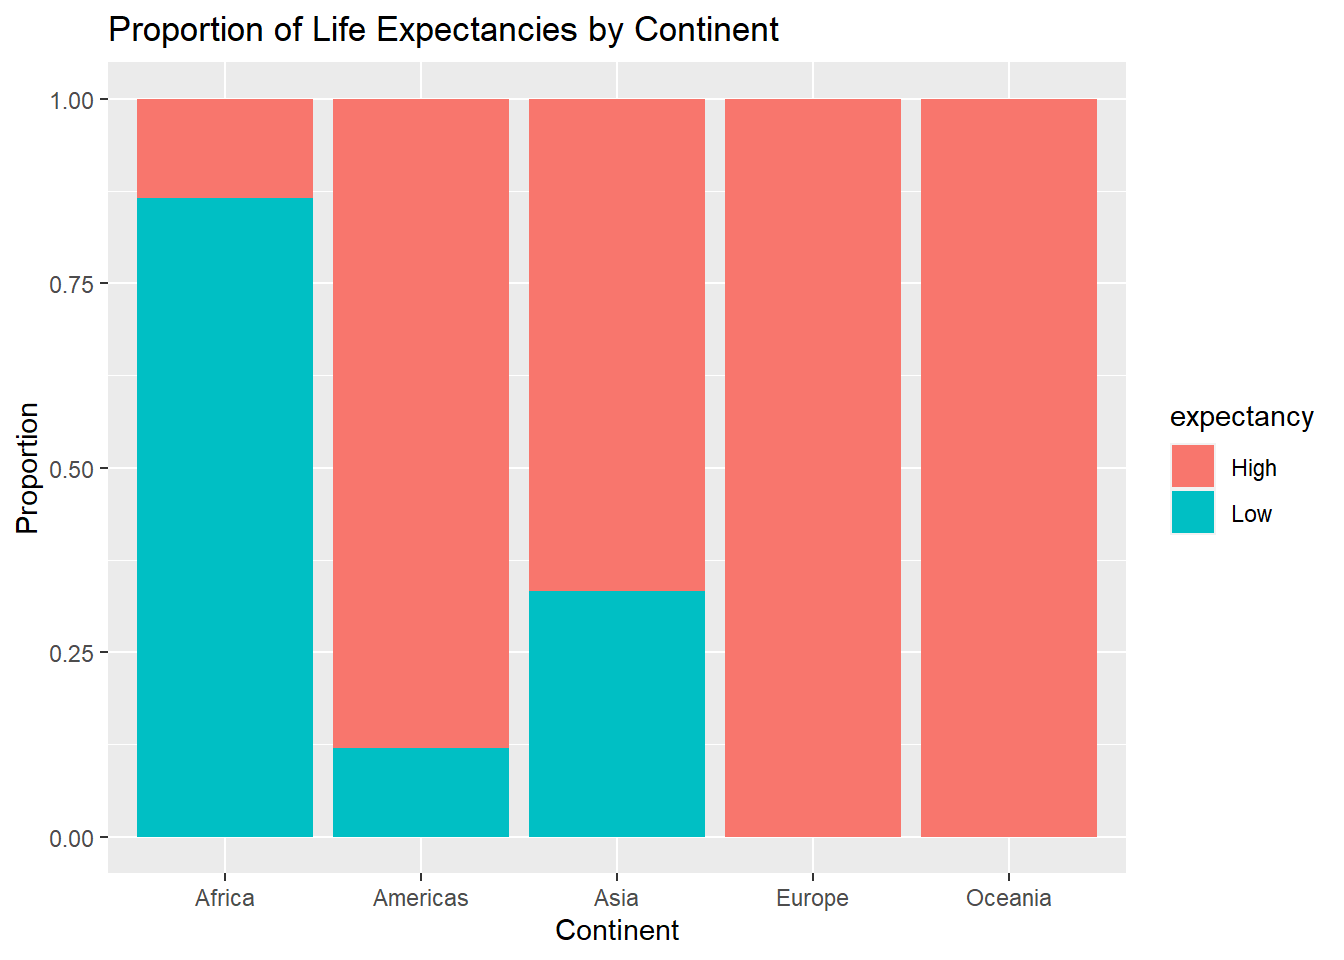
\includegraphics{bookdown-demo_files/figure-latex/unnamed-chunk-99-1.pdf}

\hypertarget{summarizing-two-quantitative-variables}{%
\subsection{Summarizing two quantitative variables}\label{summarizing-two-quantitative-variables}}

\hypertarget{scatterplots}{%
\subsubsection{Scatterplots}\label{scatterplots}}

Scatterplots are the standard visualization when two quantitative variables are involved. To create a scatterplot for life expectancy against GDP per capita:

\begin{Shaded}
\begin{Highlighting}[]
\FunctionTok{ggplot}\NormalTok{(Data, }\FunctionTok{aes}\NormalTok{(}\AttributeTok{x=}\NormalTok{gdpPercap,}\AttributeTok{y=}\NormalTok{lifeExp))}\SpecialCharTok{+}
  \FunctionTok{geom\_point}\NormalTok{()}
\end{Highlighting}
\end{Shaded}

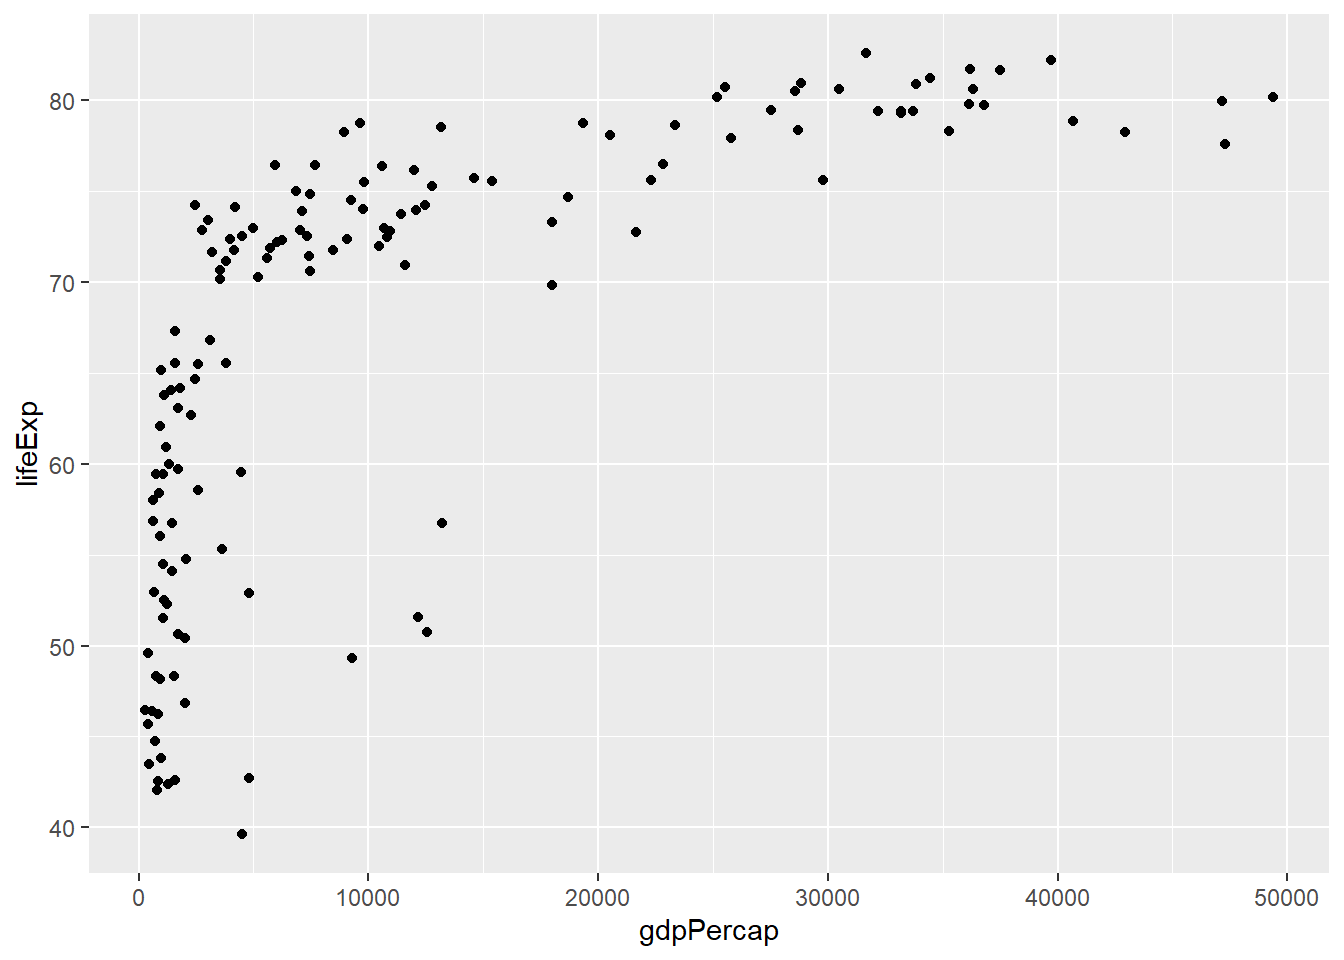
\includegraphics{bookdown-demo_files/figure-latex/unnamed-chunk-100-1.pdf}

We see a curved relationship between life expectancies and GDP per capita. Countries with higher GDP per capita tend to have longer life expectancies.

When there are many observations, plots on the scatterplot may actually overlap each other. To have a sense of how many of these exist, we can add a transparency scale called \texttt{alpha=0.2} inside \texttt{geom\_point()}:

\begin{Shaded}
\begin{Highlighting}[]
\FunctionTok{ggplot}\NormalTok{(Data, }\FunctionTok{aes}\NormalTok{(}\AttributeTok{x=}\NormalTok{gdpPercap,}\AttributeTok{y=}\NormalTok{lifeExp))}\SpecialCharTok{+}
  \FunctionTok{geom\_point}\NormalTok{(}\AttributeTok{alpha=}\FloatTok{0.2}\NormalTok{)}\SpecialCharTok{+}
  \FunctionTok{labs}\NormalTok{(}\AttributeTok{x=}\StringTok{"GDP"}\NormalTok{, }\AttributeTok{y=}\StringTok{"Life Exp"}\NormalTok{, }
       \AttributeTok{title=}\StringTok{"Scatterplot of Life Exp against GDP"}\NormalTok{)}
\end{Highlighting}
\end{Shaded}

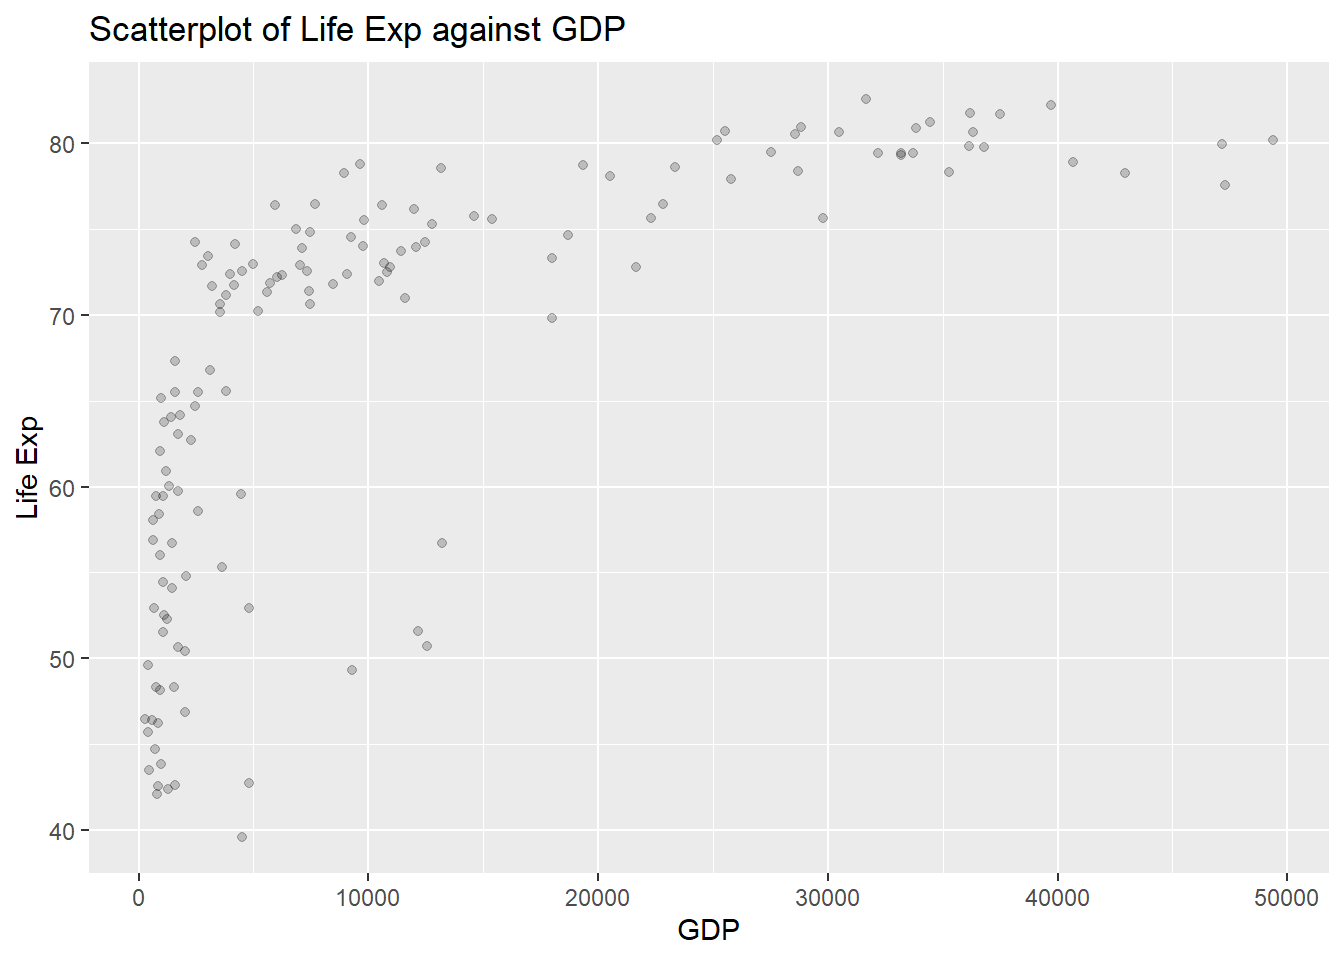
\includegraphics{bookdown-demo_files/figure-latex/unnamed-chunk-101-1.pdf}

The default value for \texttt{alpha} is 1, which means the points are not at all transparent. The closer this value is to 0, the more transparent the points are. A darker point indicates more observations with those specific values on both variables.

\hypertarget{multivariate-visualizations}{%
\section{Multivariate Visualizations}\label{multivariate-visualizations}}

We will now look at visualizations we can create to explore the relationship between multiple (more than two) variables. The term multivariate means that we are looking at more than two variables.

\hypertarget{bar-charts-2}{%
\subsection{Bar charts}\label{bar-charts-2}}

Previously, we created a bar chart to look at how \texttt{expectancy} varies across the continents. Suppose we want to see how these bar graphs vary across the years, so we use the \texttt{year} variable as a third variable via a layer \texttt{facet\_wrap}:

\begin{Shaded}
\begin{Highlighting}[]
\DocumentationTok{\#\#another data frame across all years plus a binary variable }
\DocumentationTok{\#\#for expectancy}
\NormalTok{Data.all}\OtherTok{\textless{}{-}}\NormalTok{gapminder}\SpecialCharTok{\%\textgreater{}\%}
  \FunctionTok{mutate}\NormalTok{(}\AttributeTok{expectancy=}\FunctionTok{ifelse}\NormalTok{(lifeExp}\SpecialCharTok{\textless{}}\DecValTok{70}\NormalTok{,}\StringTok{"Low"}\NormalTok{,}\StringTok{"High"}\NormalTok{))}

\FunctionTok{ggplot}\NormalTok{(Data.all,}\FunctionTok{aes}\NormalTok{(}\AttributeTok{x=}\NormalTok{continent, }\AttributeTok{fill=}\NormalTok{expectancy))}\SpecialCharTok{+}
  \FunctionTok{geom\_bar}\NormalTok{(}\AttributeTok{position =} \StringTok{"fill"}\NormalTok{)}\SpecialCharTok{+}
  \FunctionTok{facet\_wrap}\NormalTok{(}\SpecialCharTok{\textasciitilde{}}\NormalTok{year)}
\end{Highlighting}
\end{Shaded}

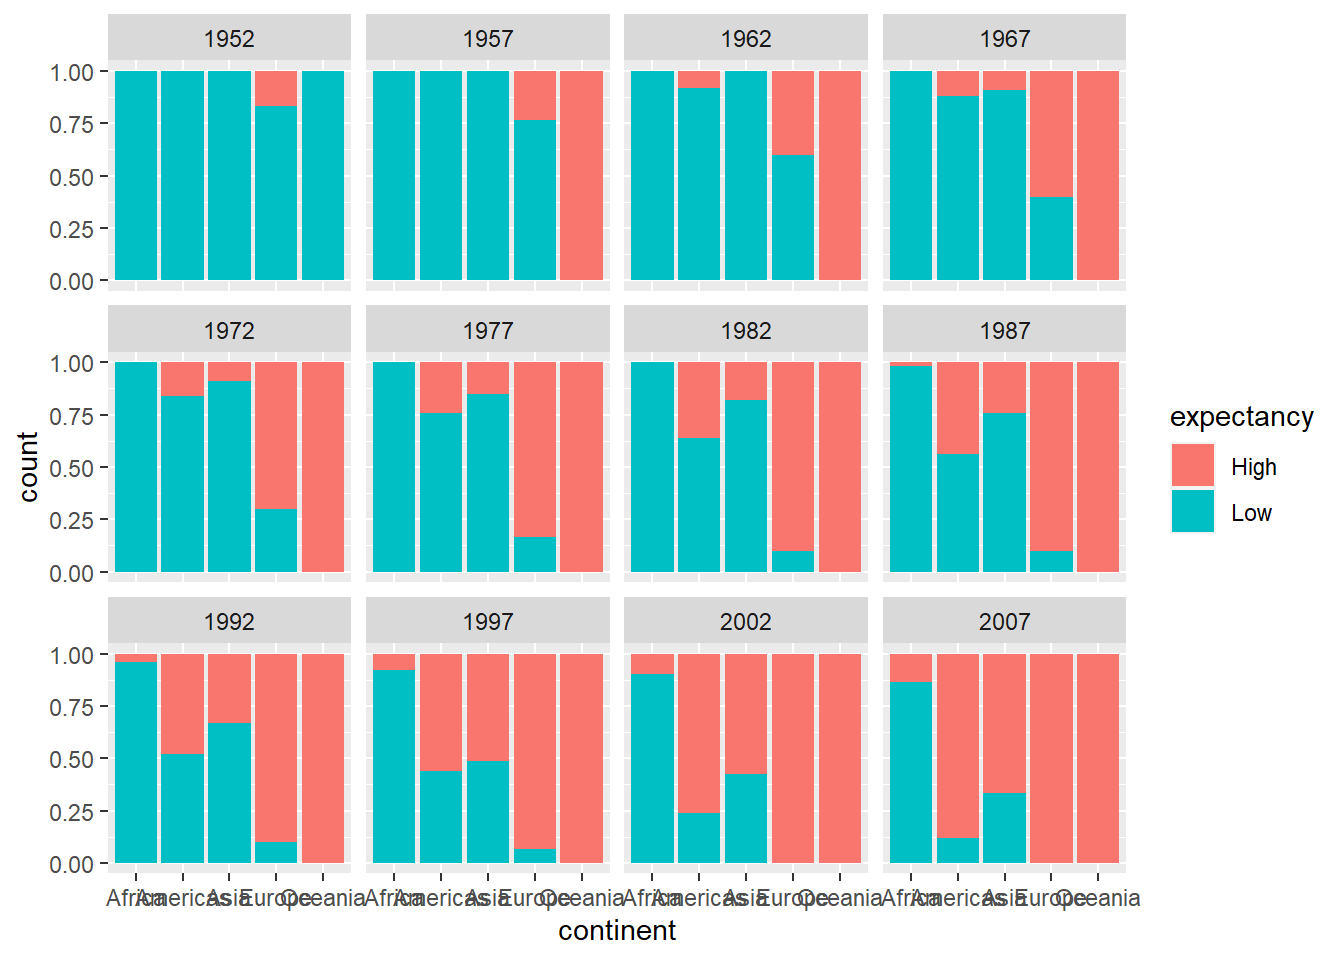
\includegraphics{bookdown-demo_files/figure-latex/unnamed-chunk-102-1.pdf}

Notice that three categorical variables are summarized in this bar chart. Is there something that can be done to improve this bar chart? How would you make this improvement?

\hypertarget{scatterplots-1}{%
\subsection{Scatterplots}\label{scatterplots-1}}

Previously, we created a scatterplot of life expectancy against GDP per capita. We can include another quantitative variable in the scatterplot, by using the size of the plots. We can use the size of the plots to denote the population of the countries. This is supplied via \texttt{size} in \texttt{aes()}:

\begin{Shaded}
\begin{Highlighting}[]
\FunctionTok{ggplot}\NormalTok{(Data, }\FunctionTok{aes}\NormalTok{(}\AttributeTok{x=}\NormalTok{gdpPercap, }\AttributeTok{y=}\NormalTok{lifeExp, }\AttributeTok{size=}\NormalTok{pop))}\SpecialCharTok{+}
  \FunctionTok{geom\_point}\NormalTok{()}
\end{Highlighting}
\end{Shaded}

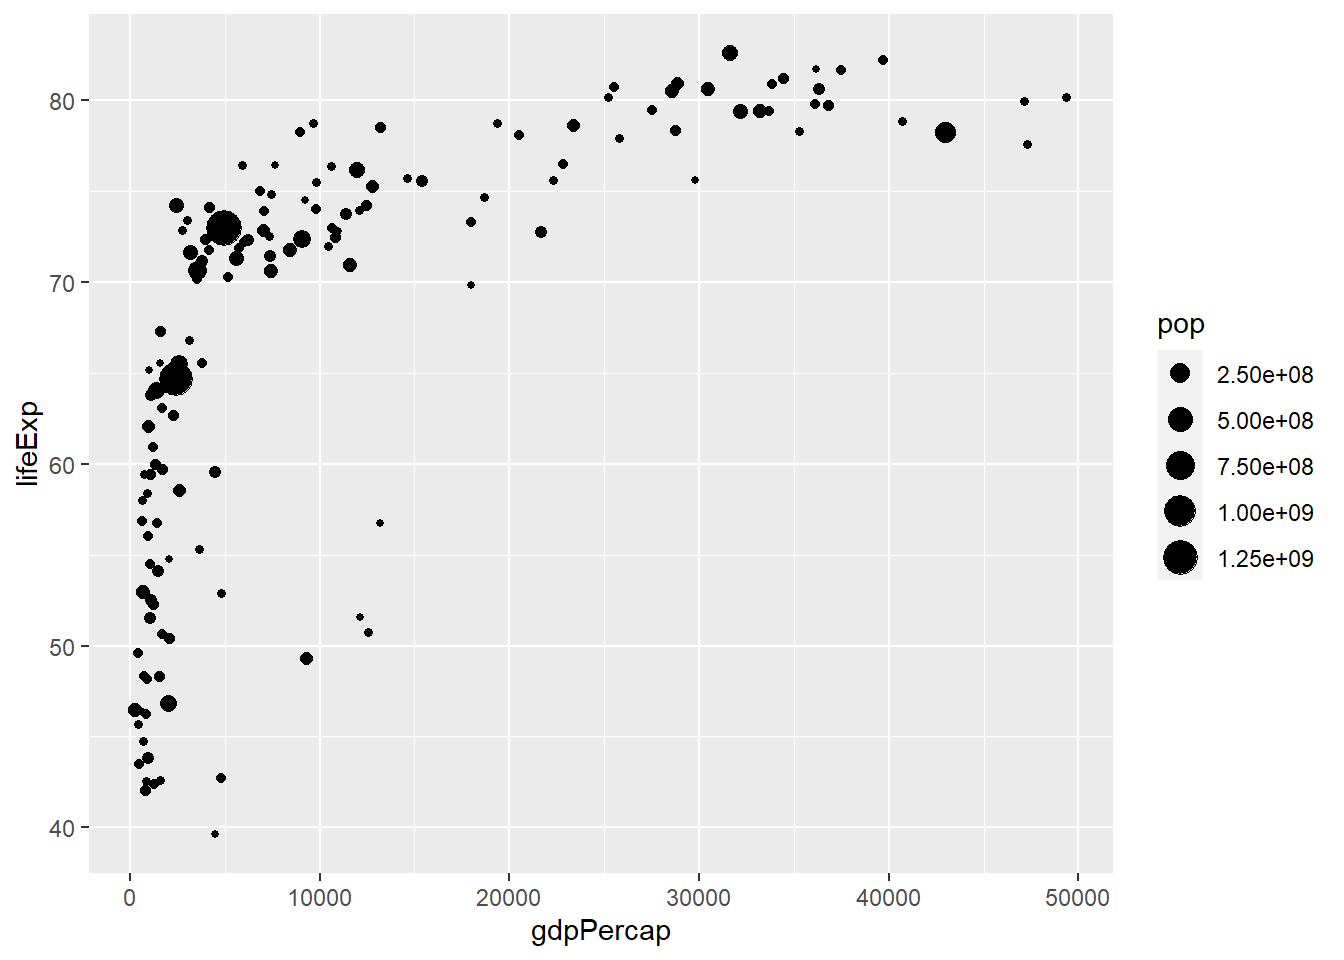
\includegraphics{bookdown-demo_files/figure-latex/unnamed-chunk-103-1.pdf}

We can adjust the size of the plots by adding a layer \texttt{scale\_size()}:

\begin{Shaded}
\begin{Highlighting}[]
\FunctionTok{ggplot}\NormalTok{(Data, }\FunctionTok{aes}\NormalTok{(}\AttributeTok{x=}\NormalTok{gdpPercap, }\AttributeTok{y=}\NormalTok{lifeExp, }\AttributeTok{size=}\NormalTok{pop))}\SpecialCharTok{+}
  \FunctionTok{geom\_point}\NormalTok{()}\SpecialCharTok{+}
  \FunctionTok{scale\_size}\NormalTok{(}\AttributeTok{range =} \FunctionTok{c}\NormalTok{(}\FloatTok{0.1}\NormalTok{,}\DecValTok{12}\NormalTok{))}
\end{Highlighting}
\end{Shaded}

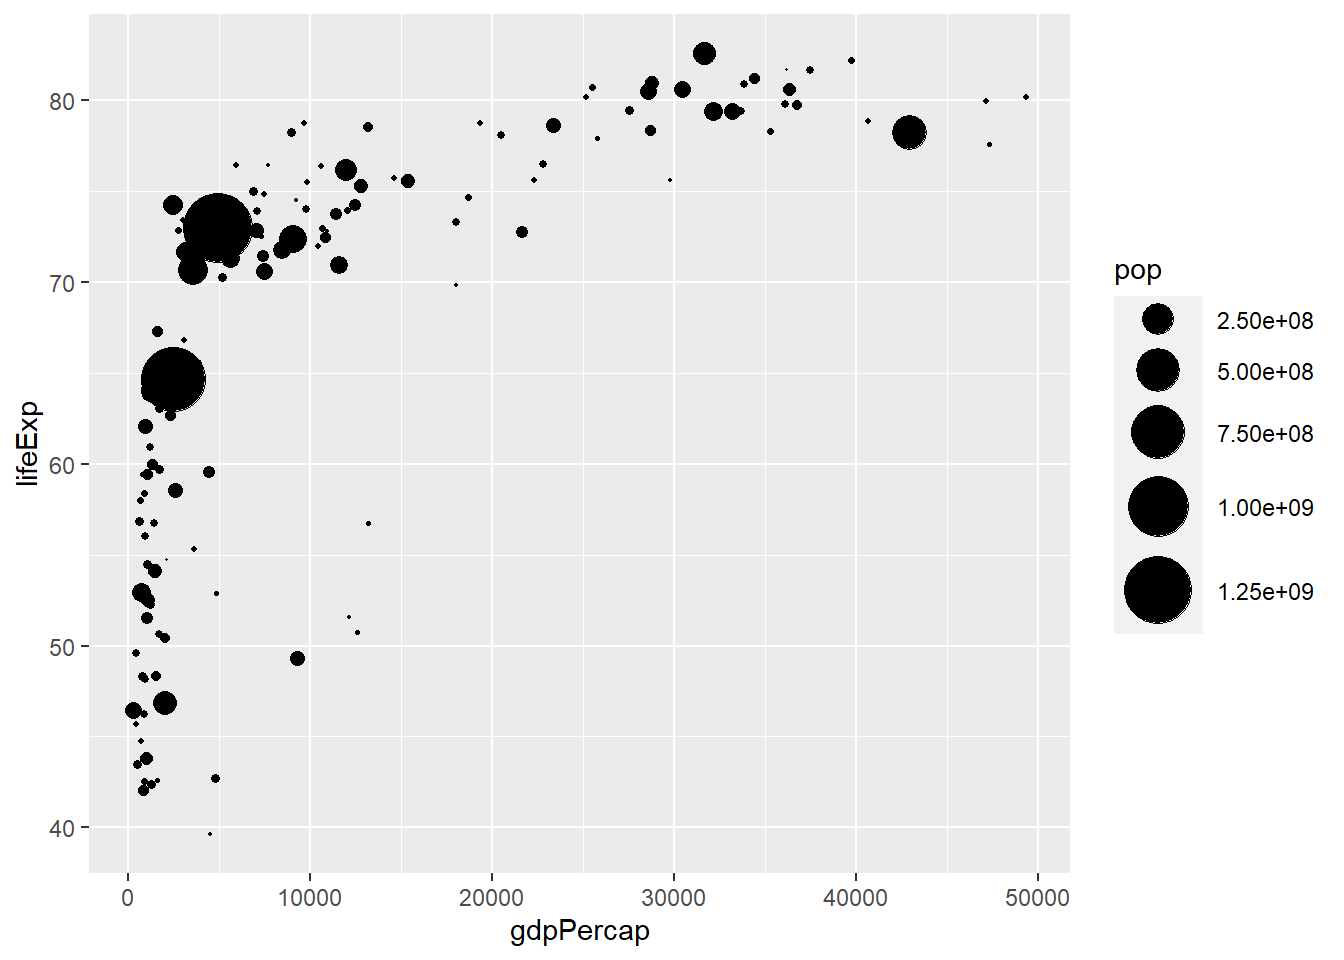
\includegraphics{bookdown-demo_files/figure-latex/unnamed-chunk-104-1.pdf}

This scatterplot summarizes three quantitative variables.

We can use different-colored plots to denote which continent each point belongs to:

\begin{Shaded}
\begin{Highlighting}[]
\FunctionTok{ggplot}\NormalTok{(Data, }\FunctionTok{aes}\NormalTok{(}\AttributeTok{x=}\NormalTok{gdpPercap, }\AttributeTok{y=}\NormalTok{lifeExp, }\AttributeTok{size=}\NormalTok{pop, }\AttributeTok{color=}\NormalTok{continent))}\SpecialCharTok{+}
  \FunctionTok{geom\_point}\NormalTok{()}\SpecialCharTok{+}
  \FunctionTok{scale\_size}\NormalTok{(}\AttributeTok{range =} \FunctionTok{c}\NormalTok{(}\FloatTok{0.1}\NormalTok{,}\DecValTok{12}\NormalTok{))}
\end{Highlighting}
\end{Shaded}

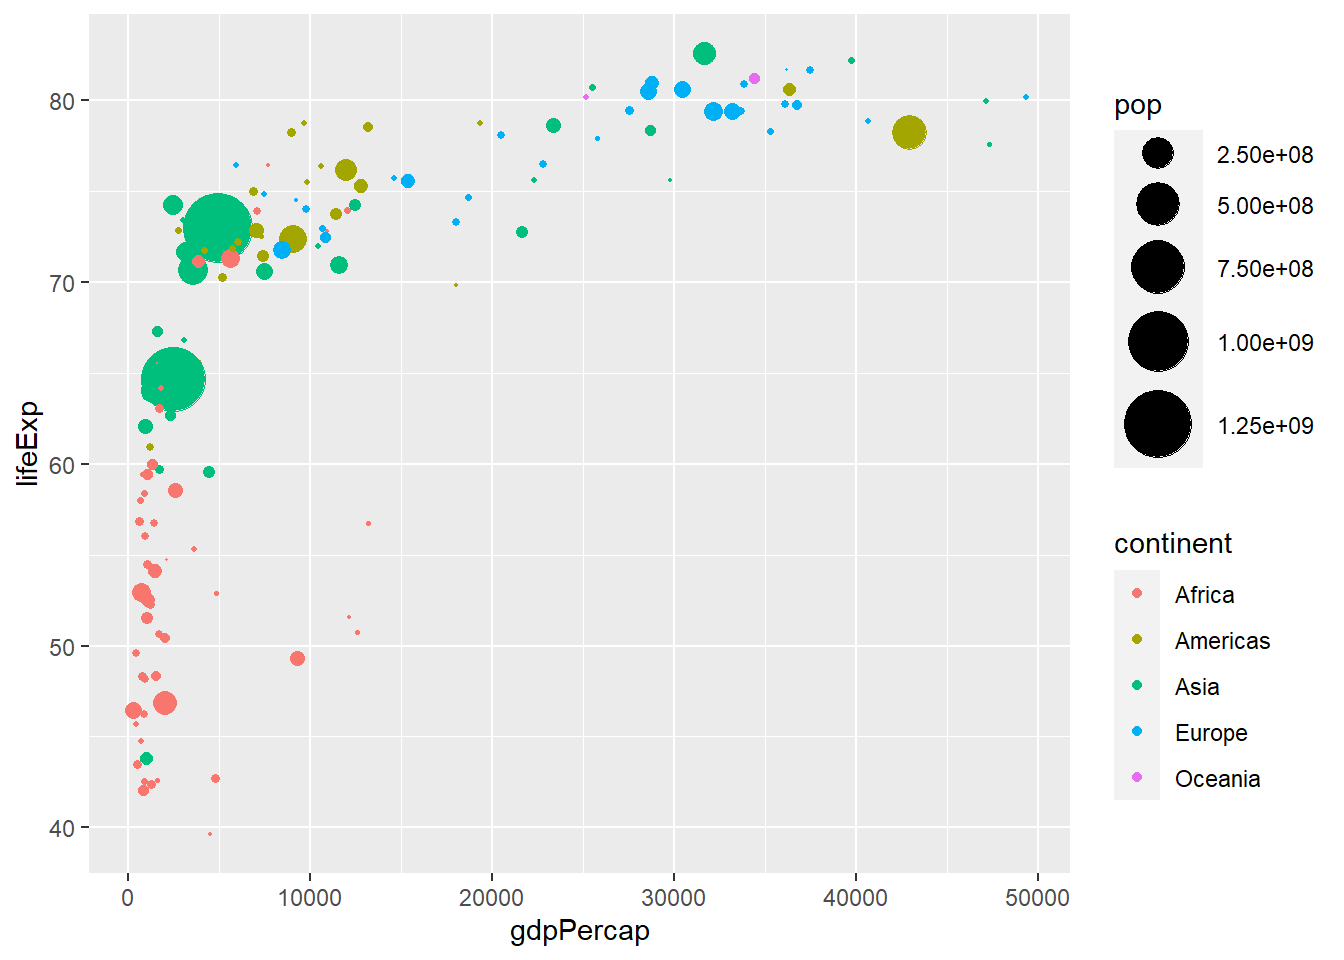
\includegraphics{bookdown-demo_files/figure-latex/unnamed-chunk-105-1.pdf}

This scatterplot summarizes three quantitative variables and one categorical variable.

We can adjust the plots by changing its shape and making it more translucent via \texttt{shape} and \texttt{alpha} in \texttt{aes()}:

\begin{Shaded}
\begin{Highlighting}[]
\FunctionTok{ggplot}\NormalTok{(Data, }\FunctionTok{aes}\NormalTok{(}\AttributeTok{x=}\NormalTok{gdpPercap, }\AttributeTok{y=}\NormalTok{lifeExp, }\AttributeTok{size=}\NormalTok{pop, }\AttributeTok{fill=}\NormalTok{continent))}\SpecialCharTok{+}
  \FunctionTok{geom\_point}\NormalTok{(}\AttributeTok{shape=}\DecValTok{21}\NormalTok{, }\AttributeTok{alpha=}\FloatTok{0.5}\NormalTok{)}\SpecialCharTok{+}
  \FunctionTok{scale\_size}\NormalTok{(}\AttributeTok{range =} \FunctionTok{c}\NormalTok{(}\FloatTok{0.1}\NormalTok{,}\DecValTok{12}\NormalTok{))}\SpecialCharTok{+}
  \FunctionTok{labs}\NormalTok{(}\AttributeTok{x=}\StringTok{"GDP"}\NormalTok{, }\AttributeTok{y=}\StringTok{"Life Exp"}\NormalTok{, }\AttributeTok{title=}\StringTok{"Scatterplot of Life Exp against GDP"}\NormalTok{)}
\end{Highlighting}
\end{Shaded}

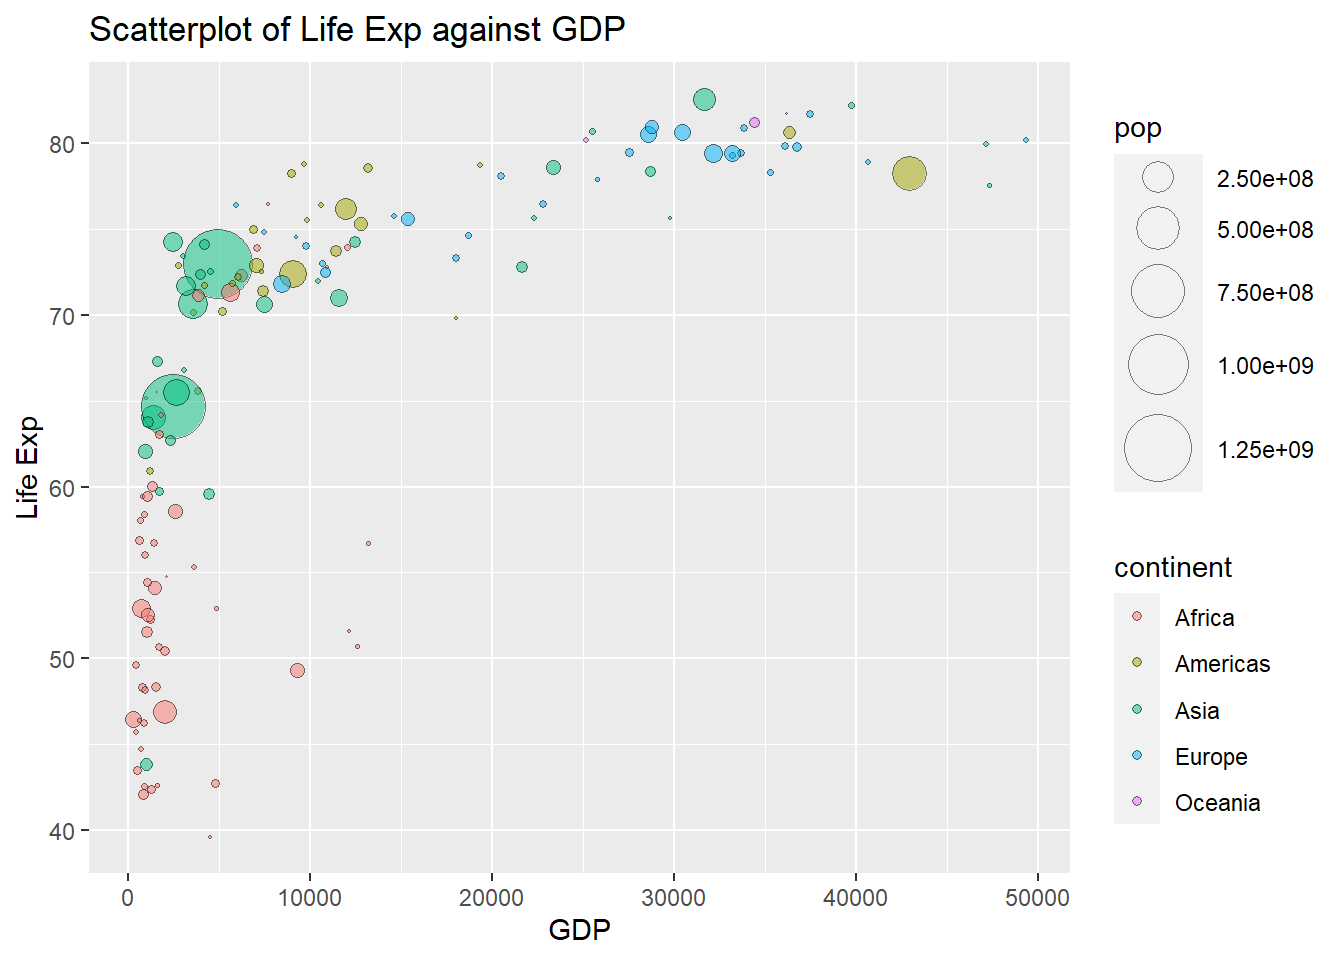
\includegraphics{bookdown-demo_files/figure-latex/unnamed-chunk-106-1.pdf}

\hypertarget{slr}{%
\chapter{Basics with Simple Linear Regression (SLR)}\label{slr}}

\hypertarget{introduction-2}{%
\section{Introduction}\label{introduction-2}}

We will start this module by introducing the simple linear regression model. Simple linear regression uses the term ``simple,'' because it concerns the study of only one predictor variable with one quantitative response variable. In contrast, multiple linear regression, which we will study in future modules, uses the term ``multiple,'' because it concerns the study of two or more predictor variables with one quantitative response variable. We start with simple linear regression as it is much easier to visualize concepts in regression models when there is only one predictor variable.

For the time being, we will only consider predictor variables that are quantitative. We will consider predictor variables that are categorical in future modules.

The most common way of visualizing the relationship between one quantitative predictor variable and one quantitative response variable is with a scatter plot. In the simulated example below, we have data from 6000 UVa undergraduate students on the amount of time they spend studying in a week (in minutes), and how many courses they are taking in the semester (3 or 4 credit courses).

\begin{Shaded}
\begin{Highlighting}[]
\DocumentationTok{\#\#create dataframe}
\NormalTok{df}\OtherTok{\textless{}{-}}\FunctionTok{data.frame}\NormalTok{(study,courses)}

\DocumentationTok{\#\#fit regression}
\NormalTok{result}\OtherTok{\textless{}{-}}\FunctionTok{lm}\NormalTok{(study}\SpecialCharTok{\textasciitilde{}}\NormalTok{courses, }\AttributeTok{data=}\NormalTok{df)}
\end{Highlighting}
\end{Shaded}

\begin{Shaded}
\begin{Highlighting}[]
\DocumentationTok{\#\#create scatterplot with regression line overlaid}
\FunctionTok{plot}\NormalTok{(df}\SpecialCharTok{$}\NormalTok{courses, df}\SpecialCharTok{$}\NormalTok{study, }\AttributeTok{xlab=}\StringTok{"\# of Courses"}\NormalTok{, }\AttributeTok{ylab=}\StringTok{"Study Time (Mins)"}\NormalTok{)}
\FunctionTok{abline}\NormalTok{(result)}
\end{Highlighting}
\end{Shaded}

\begin{figure}
\centering
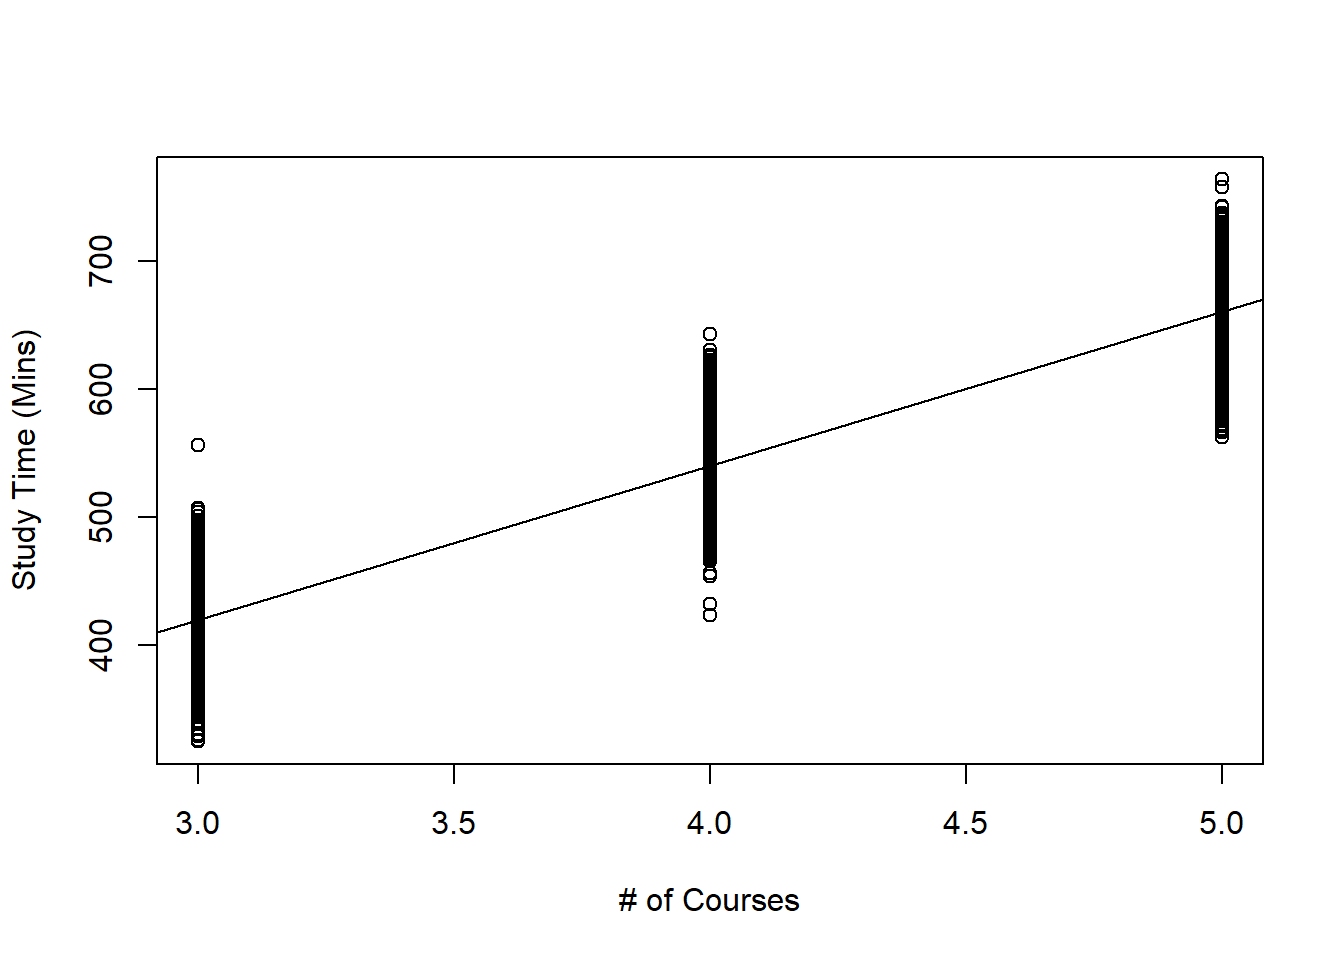
\includegraphics{bookdown-demo_files/figure-latex/scatter-courses-1.pdf}
\caption{\label{fig:scatter-courses}Scatterplot of Study Time against Number of Courses Taken}
\end{figure}

Questions that we may have include:

\begin{itemize}
\tightlist
\item
  Are study time and the number of courses taken related to one another?
\item
  How strong is this relationship?
\item
  Could we use the data to make a prediction for the study time of a student who is not in this scatterplot?
\item
  How confident are we of the prediction?
\end{itemize}

These questions can be answered using simple linear regression.

Note that we will only be learning about models with just one response variable. We will not cover multivariate regression, which is used when there is more than one response variable. There may be some confusion between ``multiple'' linear regression and ``multivariate'' regression due to the closeness in terminology.

\hypertarget{basic-ideas-with-statistics}{%
\subsection{Basic Ideas with Statistics}\label{basic-ideas-with-statistics}}

\hypertarget{population-vs-sample}{%
\subsubsection{Population vs Sample}\label{population-vs-sample}}

Statistical methods are usually used to make inferences about the \textbf{population} based on information from a \textbf{sample}.

\begin{itemize}
\tightlist
\item
  A sample is the collection of units that is actually measured or surveyed in a study.
\item
  The population includes all units of interest.
\end{itemize}

In the study time example above, the population is all UVa undergraduate students, while the sample is the 6000 students that we have data on and are displayed on the scatterplot.

\hypertarget{parameters-vs-statistics}{%
\subsubsection{Parameters vs Statistics}\label{parameters-vs-statistics}}

\begin{itemize}
\tightlist
\item
  \textbf{Parameters} are numerical quantities that describe a population.
\item
  \textbf{Statistics} are numerical quantities that describe a sample.
\end{itemize}

In the study time example, an example of a parameter will be the average study time among all UVa undergraduate students (called the population mean), and an example of a statistic will be the average study time among the 6000 UVa students we have data on (called the sample mean).

Notice that in real life, we will rarely know the actual numerical value of a parameter. So we use the numerical value of the statistic to \textbf{estimate} the unknown numerical value of the corresponding parameter.

We also have different notation for parameters and statistics. For example,

\begin{itemize}
\tightlist
\item
  the population mean is denoted as \(\mu\).
\item
  the sample mean is denoted as \(\bar{x}\).
\end{itemize}

We say that \(\bar{x}\) is an \textbf{estimator} of \(\mu\).

It is important to pay attention to whether we are describing a statistic (a known value that can be calculated) or a parameter (an unknown value).

\hypertarget{motivation}{%
\subsection{Motivation}\label{motivation}}

Linear regression models generally have two primary uses:

\begin{enumerate}
\def\labelenumi{\arabic{enumi}.}
\tightlist
\item
  \textbf{Prediction}: Predict a future value of a response variable, using information from predictor variables.
\item
  \textbf{Association}: Quantify the relationship between variables. How does a change in the predictor variable change the value of the response variable?
\end{enumerate}

We always distinguish between a \textbf{response variable, denoted by \(y\)}, and a \textbf{predictor variable, denoted by \(x\)}. In most statistical models, we say that the response variable can be approximated by some \textbf{mathematical function, denoted by \(f\)}, of the predictor variable, i.e.

\[
y \approx f(x).
\]
Oftentimes, we write this relationship as

\[
y = f(x) + \epsilon,
\]

where \textbf{\(\epsilon\) denotes a random error term}, with a mean of 0. The error term cannot be predicted based on the data we have.

There are various statistical methods to estimate \(f\). Once we estimate \(f\), we can use our method for prediction and / or association.

Using the study time example above:

\begin{itemize}
\tightlist
\item
  a prediction example: a student intends to take 4 courses in the semester. What is this student's predicted study time, on average?
\item
  an association example: we want to see how taking more courses increases study time.
\end{itemize}

\hypertarget{practice-questions}{%
\subsubsection{Practice questions}\label{practice-questions}}

In the examples below, are we using a regression model for prediction or for association?

\begin{enumerate}
\def\labelenumi{\arabic{enumi}.}
\item
  It is early in the morning and I am heading out for the rest of the day. I want to know the weather forecast for the rest of the day so I know what to wear.
\item
  An executive for a sports league wants to assess how increasing the length of commercial breaks may impact the enjoyment of sports fans who watch games on TV.
\item
  The Education Secretary would like to evaluate how certain factors such as use of technology in classrooms and investment in teacher training and teacher pay are associated with reading skills of students.
\item
  When buying a home, the prospective buyer would like to know if the home is under- or over- priced, given its characteristics.
\end{enumerate}

\hypertarget{simple-linear-regression-slr}{%
\section{Simple Linear Regression (SLR)}\label{simple-linear-regression-slr}}

In simple linear regression (SLR), the function \(f\) that relates the predictor variable with the response variable is typically \(\beta_0 + \beta_1 x\). Mathematically, we express this as

\[
y \approx \beta_0 + \beta_1 x,
\]

or in other words, that the response variable has an approximately linear relationship with the predictor variable.

In SLR, this relationship is more explicitly formulated as the \textbf{simple linear regression equation}:

\begin{equation} 
E(y|x)=\beta_0+\beta_{1}x.
\label{eq:SLR}
\end{equation}

\begin{itemize}
\item
  \(\beta_0\) and \(\beta_1\) are parameters in the SLR equation, and we want to estimate them.
\item
  These parameters are sometimes called \textbf{regression coefficients}.
\item
  \(\beta_1\) is also called the \textbf{slope. It denotes the change in \(y\), on average, when \(x\) increases by one unit.}
\item
  \(\beta_0\) is also called the \textbf{intercept. It denotes the average of \(y\) when \(x=0\).}
\item
  The notation on the left hand side of \eqref{eq:SLR} denotes the \textbf{expected value} of the response variable, for a fixed value of the predictor variable. What \eqref{eq:SLR} implies is that, for each value of the predictor variable \(x\), the expected value of the response variable \(y\) is \(\beta_0+\beta_{1}x\). The expected value is also the population mean. Applying \eqref{eq:SLR} to our study time example, it implies that:

  \begin{itemize}
  \tightlist
  \item
    for students who take 3 courses, their expected study time is equal to \(\beta_0 + 3\beta_1\),
  \item
    for students who take 4 courses, their expected study time is equal to \(\beta_0 + 4\beta_1\),
  \item
    for students who take 5 courses, their expected study time is equal to \(\beta_0 + 5\beta_1\).
  \end{itemize}
\end{itemize}

So \(f(x) = \beta_0 + \beta_1x\) gives us the value of the expected value of the response variable for a specific value of the predictor variable. But, for each value of the predictor variable, the value of the response variable is not a constant. We say that for each value of \(x\), the response variable \(y\) has some variance. The variance of the response variable for each value of \(x\) is the same as the variance of the error term, \(\epsilon\). Thus we have the \textbf{simple linear regression model}

\begin{equation} 
y=\beta_0+\beta_{1} x + \epsilon. 
\label{eq:SLRmod}
\end{equation}

We need to make some assumptions for the error term \(\epsilon\). Generally, the assumptions are:

\begin{enumerate}
\def\labelenumi{\arabic{enumi}.}
\tightlist
\item
  The errors have mean 0.
\item
  The \textbf{errors have variance denoted by \(\sigma^2\)}. Notice this variance is constant.
\item
  The errors are independent.
\item
  The errors are normally distributed.
\end{enumerate}

From \eqref{eq:SLRmod}, notice we have another parameter, \(\sigma^2\).

We will go into more detail about what these assumptions mean, and how to assess whether they are met, in module \ref{diag}.

What these assumptions mean is that for each value of the predictor variable \(x\), the response variable:

\begin{enumerate}
\def\labelenumi{\arabic{enumi}.}
\tightlist
\item
  follows a normal distribution,
\item
  with mean equal to \(\beta_0+\beta_{1} x\),
\item
  and variance equal to \(\sigma^2\).
\end{enumerate}

Using our study time example, it means that:

\begin{itemize}
\tightlist
\item
  for students who take 3 courses, the distribution of their study times is \(N(\beta_0 + 3\beta_1, \sigma^2)\).
\item
  for students who take 4 courses, the distribution of their study times is \(N(\beta_0 + 4\beta_1, \sigma^2)\).
\item
  for students who take 5 courses, the distribution of their study times is \(N(\beta_0 + 5\beta_1, \sigma^2)\).
\end{itemize}

So if we were to subset our dataframe into three subsets, one with students who take 3 courses, another subset for students who take 4 courses, and another subset for students who take 5 courses, and then create a density plot of study times for each subset, each density plot should follow a normal distribution, with different means, and the same spread.

Let us take a look at these density plots next.

\begin{Shaded}
\begin{Highlighting}[]
\FunctionTok{library}\NormalTok{(tidyverse)}
\end{Highlighting}
\end{Shaded}

\begin{Shaded}
\begin{Highlighting}[]
\DocumentationTok{\#\#subset dataframe}
\NormalTok{x}\FloatTok{.3}\OtherTok{\textless{}{-}}\NormalTok{df[}\FunctionTok{which}\NormalTok{(df}\SpecialCharTok{$}\NormalTok{courses}\SpecialCharTok{==}\DecValTok{3}\NormalTok{),]}
\DocumentationTok{\#\#density plot of study time for students taking 3 courses}
\FunctionTok{ggplot}\NormalTok{(x}\FloatTok{.3}\NormalTok{,}\FunctionTok{aes}\NormalTok{(}\AttributeTok{x=}\NormalTok{study))}\SpecialCharTok{+}
  \FunctionTok{geom\_density}\NormalTok{()}\SpecialCharTok{+}
  \FunctionTok{labs}\NormalTok{(}\AttributeTok{x=}\StringTok{"Study Time (Mins)"}\NormalTok{, }\AttributeTok{title=}\StringTok{"Dist of Study Times with 3 Courses"}\NormalTok{)}
\end{Highlighting}
\end{Shaded}

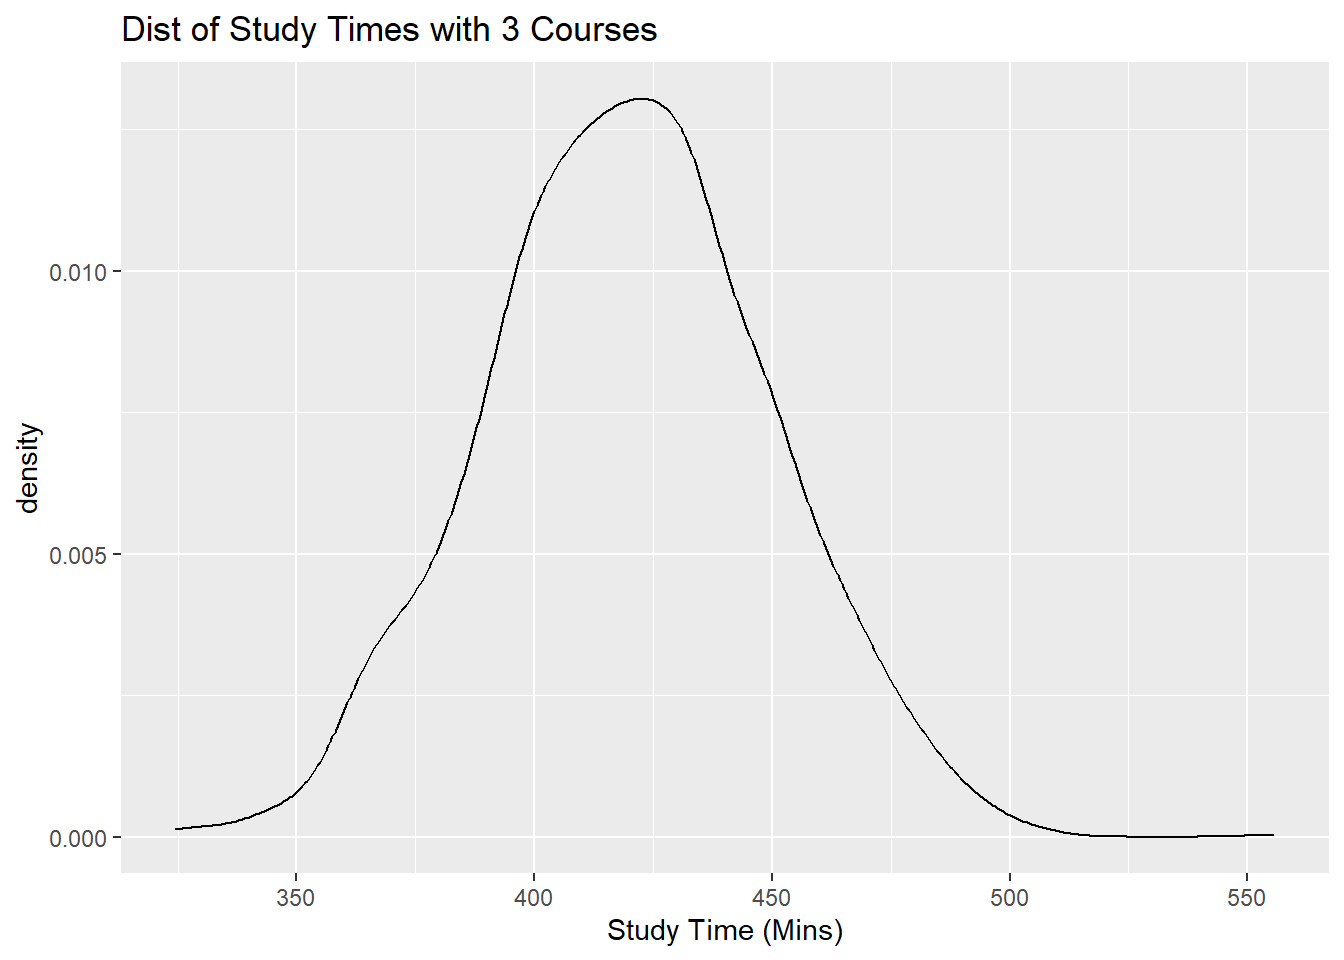
\includegraphics{bookdown-demo_files/figure-latex/unnamed-chunk-111-1.pdf}

\begin{Shaded}
\begin{Highlighting}[]
\DocumentationTok{\#\#subset dataframe}
\NormalTok{x}\FloatTok{.4}\OtherTok{\textless{}{-}}\NormalTok{df[}\FunctionTok{which}\NormalTok{(df}\SpecialCharTok{$}\NormalTok{courses}\SpecialCharTok{==}\DecValTok{4}\NormalTok{),]}
\DocumentationTok{\#\#density plot of study time for students taking 4 courses}
\FunctionTok{ggplot}\NormalTok{(x}\FloatTok{.4}\NormalTok{,}\FunctionTok{aes}\NormalTok{(}\AttributeTok{x=}\NormalTok{study))}\SpecialCharTok{+}
  \FunctionTok{geom\_density}\NormalTok{()}\SpecialCharTok{+}
  \FunctionTok{labs}\NormalTok{(}\AttributeTok{x=}\StringTok{"Study Time (Mins)"}\NormalTok{, }\AttributeTok{title=}\StringTok{"Dist of Study Times with 4 Courses"}\NormalTok{)}
\end{Highlighting}
\end{Shaded}

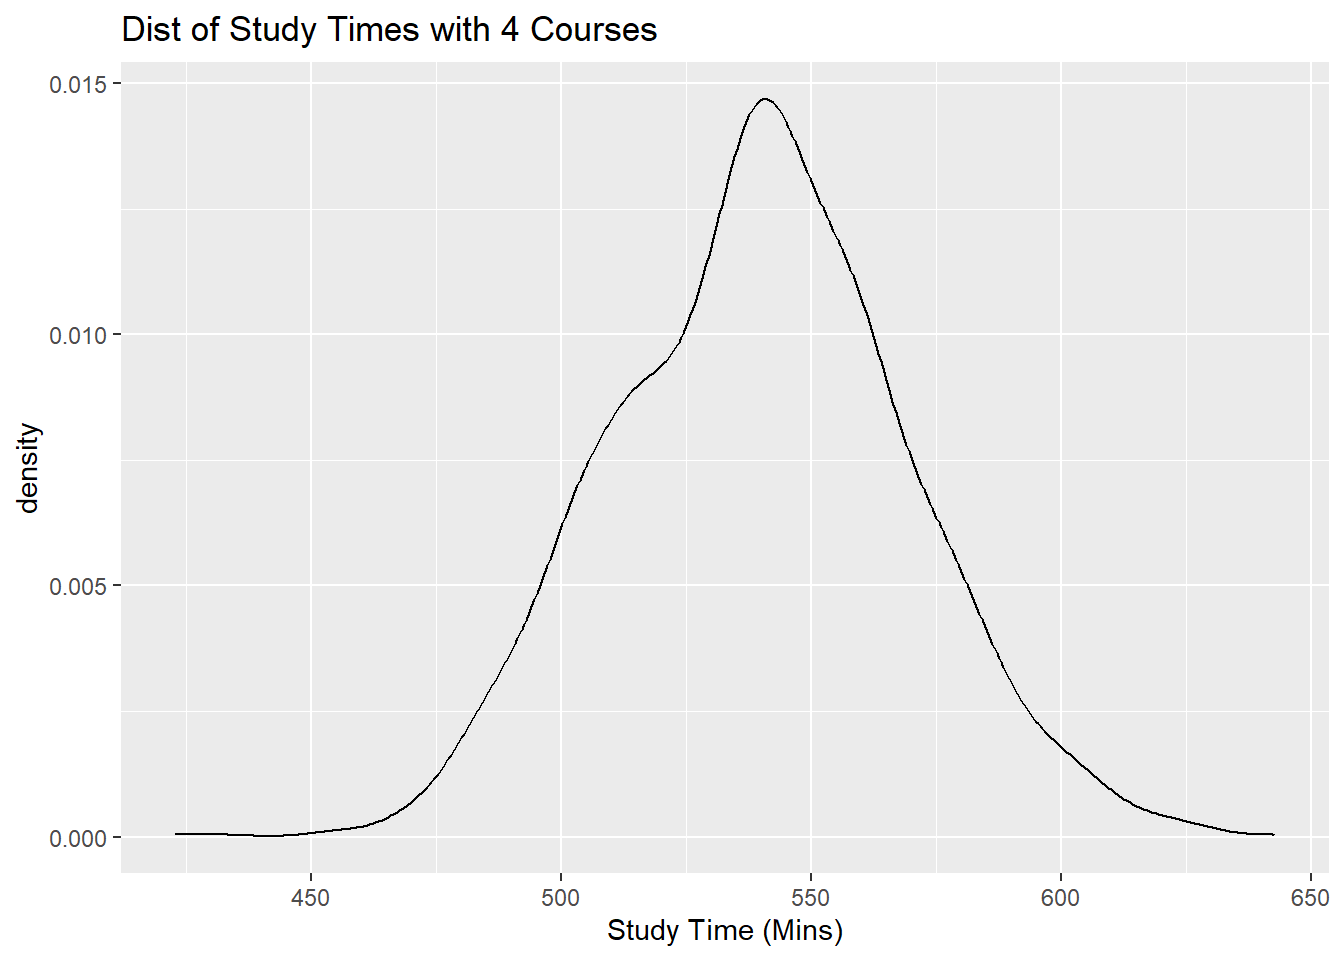
\includegraphics{bookdown-demo_files/figure-latex/unnamed-chunk-111-2.pdf}

\begin{Shaded}
\begin{Highlighting}[]
\DocumentationTok{\#\#subset dataframe}
\NormalTok{x}\FloatTok{.5}\OtherTok{\textless{}{-}}\NormalTok{df[}\FunctionTok{which}\NormalTok{(df}\SpecialCharTok{$}\NormalTok{courses}\SpecialCharTok{==}\DecValTok{5}\NormalTok{),]}
\DocumentationTok{\#\#density plot of study time for students taking 5 courses}
\FunctionTok{ggplot}\NormalTok{(x}\FloatTok{.5}\NormalTok{,}\FunctionTok{aes}\NormalTok{(}\AttributeTok{x=}\NormalTok{study))}\SpecialCharTok{+}
  \FunctionTok{geom\_density}\NormalTok{()}\SpecialCharTok{+}
  \FunctionTok{labs}\NormalTok{(}\AttributeTok{x=}\StringTok{"Study Time (Mins)"}\NormalTok{, }\AttributeTok{title=}\StringTok{"Dist of Study Times with 5 Courses"}\NormalTok{)}
\end{Highlighting}
\end{Shaded}

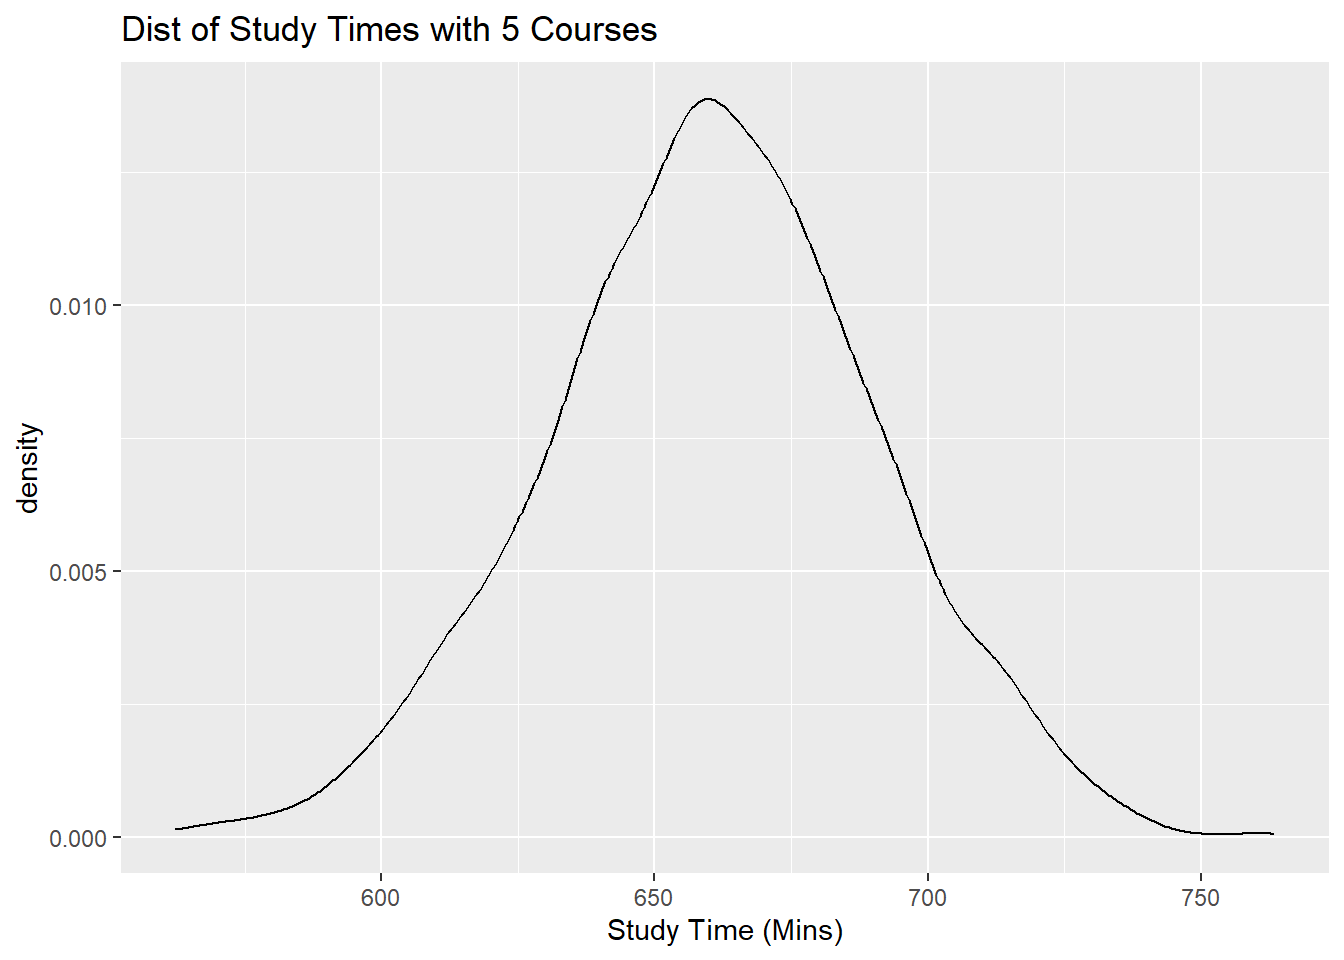
\includegraphics{bookdown-demo_files/figure-latex/unnamed-chunk-111-3.pdf}

Notice all of these plots are normal, with different means (centers), and similar spreads.

\emph{Please see the associated video for more explanation about the distribution of the response variable, for each value of the predictor variable, in an SLR setting.}

\hypertarget{estimating-regression-coefficients-in-slr}{%
\section{Estimating Regression Coefficients in SLR}\label{estimating-regression-coefficients-in-slr}}

From \eqref{eq:SLR} and \eqref{eq:SLRmod}, we noted that we have to estimate the regression coefficients \(\beta_0, \beta_1\) as well as the parameter \(\sigma^2\) associated with the error term. As mentioned earlier, we are unable to obtain numerical values of these parameters as we do not have data from the entire population. So what we do is use the data from our sample to estimate these parameters.

We estimate \(\beta_0,\beta_1\) using \(\hat{\beta}_0,\hat{\beta}_1\) based on a sample of observations \((x_i,y_i)\) of size \(n\).

The subscripts associated with the response and predictor variables denote which data point that value belongs to. Let us take a look at the first few rows of the data frame for the study time example:

\begin{Shaded}
\begin{Highlighting}[]
\FunctionTok{head}\NormalTok{(df)}
\end{Highlighting}
\end{Shaded}

\begin{verbatim}
##      study courses
## 1 429.8311       3
## 2 458.4588       3
## 3 391.9406       3
## 4 378.0196       3
## 5 397.9856       3
## 6 405.7145       3
\end{verbatim}

For example, \(x_1\) denotes the number of courses taken by student number 1 in the dataframe, which is 3. \(y_4\) denotes the study time for student number 4 in the dataframe, which is 378.0196456.

Following \eqref{eq:SLR} and \eqref{eq:SLRmod}, the sample versions are

\begin{equation} 
\hat{y}=\hat{\beta}_0+\hat{\beta}_1 x
\label{eq:fitted}
\end{equation}

and

\begin{equation} 
y=\hat{\beta}_0+\hat{\beta}_1 x + e
\label{eq:fitted-model}
\end{equation}

respectively. \eqref{eq:fitted} is called the \textbf{estimated SLR equation}, or \textbf{fitted SLR equation}. \eqref{eq:fitted-model} is called the \textbf{estimated SLR model}.

\(\hat{\beta}_1,\hat{\beta}_0\) are the estimators for \(\beta_1,\beta_0\) respectively. These estimators can be interpreted in the following manner:

\begin{itemize}
\tightlist
\item
  \textbf{\(\hat{\beta}_1\) denotes the change in the predicted \(y\) when \(x\) increases by 1 unit. Alternatively, it denotes the change in \(y\), on average, when \(x\) increases by 1 unit.}
\item
  \textbf{\(\hat{\beta}_0\) denotes the predicted \(y\) when \(x=0\). Alternatively, it denotes the average of \(y\) when \(x=0\).}
\end{itemize}

From \eqref{eq:fitted-model}, notice we use \textbf{\(e\) to denote the residual}, or in other words, the ``error'' in the sample.

From \eqref{eq:fitted} and \eqref{eq:fitted-model}, we have the following quantities that we can compute:

\begin{equation}
\text{Predicted/Fitted values: } \hat{y}_i = \hat{\beta}_0+\hat{\beta}_1 x_i.
\label{eq:fits}
\end{equation}

\begin{equation} 
\text{Residuals: } e_i = y_i-\hat{y}_i.
\label{eq:res}
\end{equation}

\begin{equation} 
\text{Sum of Squared Residuals: } SS_{res} =  \sum\limits_{i=1}^n(y_i-\hat{y}_i)^2.
\label{eq:SSres}
\end{equation}

We compute the estimated coefficients \(\hat{\beta}_1,\hat{\beta}_0\) using the \textbf{method of least squares}, i.e.~choose the numerical values of \(\hat{\beta}_1,\hat{\beta}_0\) that minimize \(SS_{res}\) as given in \eqref{eq:SSres}.

By minimizing \(SS_{res}\) with respect to \(\hat{\beta}_0\) and \(\hat{\beta}_1\), the estimated coefficients in the simple linear regression equation are

\begin{equation} 
\hat{\beta}_1 = \frac{\sum\limits_{i=1}^n(x_i-\bar{x})(y_i-\bar{y})}{\sum\limits_{i=1}^n(x_i-\bar{x})^2}
\label{eq:b1}
\end{equation}

and

\begin{equation} 
\hat{\beta}_0 = \bar{y}- \hat{\beta}_1 \bar{x}
\label{eq:b0}
\end{equation}

\(\hat{\beta}_1, \hat{\beta}_0\) are called \textbf{least squares estimators}.

The minimization of \(SS_{res}\) with respect to \(\hat{\beta}_0\) and \(\hat{\beta}_1\) is done by taking the partial derivatives of \eqref{eq:SSres} with respect to \(\hat{\beta}_1\) and \(\hat{\beta}_0\), setting these two partial derivatives equal to 0, and solving these two equations for \(\hat{\beta}_1\) and \(\hat{\beta}_0\).

Let's take a look at the estimated coefficients for our study time example:

\begin{Shaded}
\begin{Highlighting}[]
\DocumentationTok{\#\#fit regression}
\NormalTok{result}\OtherTok{\textless{}{-}}\FunctionTok{lm}\NormalTok{(study}\SpecialCharTok{\textasciitilde{}}\NormalTok{courses, }\AttributeTok{data=}\NormalTok{df)}
\DocumentationTok{\#\#print out the estimated coefficients}
\NormalTok{result}
\end{Highlighting}
\end{Shaded}

\begin{verbatim}
## 
## Call:
## lm(formula = study ~ courses, data = df)
## 
## Coefficients:
## (Intercept)      courses  
##       58.45       120.39
\end{verbatim}

From our sample of 6000 students, we have

\begin{itemize}
\tightlist
\item
  \(\hat{\beta}_1\) = 120.3930985. The predicted study time increases by 120.3930985 minutes for each additional course taken.
\item
  \(\hat{\beta}_0\) = 58.4482853. The predicted study time is 58.4482853 when no courses are taken. Notice this value does not make sense, as a student cannot be taking 0 courses. If you look at our data, the number of courses taken is 3, 4, or 5. So we should only use our regression when \(3 \leq x \leq 5\). We cannot use it for values of \(x\) outside the range of our data. Making predictions of the response variable for predictors outside the range of the data is called \textbf{extrapolation} and should not be done.
\end{itemize}

\hypertarget{estimating-variance-of-errors-in-slr}{%
\section{Estimating Variance of Errors in SLR}\label{estimating-variance-of-errors-in-slr}}

The estimator of \(\sigma^2\), the variance of the error terms (also the variance of the probability distribution of \(y\) given \(x\)) is
\begin{equation} 
s^2 = MS_{res} = \frac{SS_{res}}{n-2} = \frac{\sum\limits_{i=1}^n e_i^2}{n-2},
\label{eq:variance}
\end{equation}

where \(MS_{res}\) is the called the \textbf{mean squared residuals}.

\(\sigma^2\), the variance of the error terms, measures the spread of the response variable, for each value of \(x\). The smaller this is, the closer the data points are to the regression equation.

\hypertarget{practice-questions-1}{%
\subsection{Practice questions}\label{practice-questions-1}}

Take a look at the scatterplot of study time against number of courses taken, Figure \ref{fig:scatter-courses}. On this plot, label the following:

\begin{itemize}
\tightlist
\item
  estimated SLR equation
\item
  the fitted value when \(x=3\), \(x=4\), and \(x=5\).
\item
  the residual for any data point on the plot of your choosing.
\end{itemize}

\emph{Try these on your own first, then view the associated video to see if you labeled the plot correctly!}

\hypertarget{assessing-linear-association}{%
\section{Assessing Linear Association}\label{assessing-linear-association}}

As noted earlier, the variance of the error terms inform us how close the data points are to the estimated SLR equation. The smaller the variance of the error terms, the closer the data points are to the estimated SLR equation. This in turn implies the linear relationship between the variables is stronger.

We will learn about some common measures that are used to quantify the strength of the linear relationship between the response and predictor variables. Before we do that, we need to define some other terms.

\hypertarget{sum-of-squares}{%
\subsection{Sum of squares}\label{sum-of-squares}}

\begin{equation} 
\text{Total Sum of Squares: } SS_T = \sum\limits_{i=1}^{n} (y_i - \bar{y})^{2}.
\label{eq:SST}
\end{equation}

Total sum of squares is defined as the \textbf{total variance in the response variable}. The larger this value is, the larger the spread is of the response variable.

\begin{equation} 
\text{Regression sum of squares: } SS_R = \sum\limits_{i=1}^{n} (\hat{y_i} - \bar{y})^{2}.
\label{eq:SSR}
\end{equation}

Regression sum of squares is defined as the \textbf{variance in the response variable that can be explained by our regression}.

We also have residual sum of squares, \(SS_{res}\). Its mathematical formulation is given in \eqref{eq:SSres}. It is defined as the \textbf{variance in the response variable that cannot be explained by our regression}.

It can be shown that

\begin{equation}
SS_T = SS_R + SS_{res}.
\label{eq:SS}
\end{equation}

Each of the sums of squares has its associated \textbf{degrees of freedom (df)}:

\begin{itemize}
\tightlist
\item
  df for \(SS_R\): \(df_R = 1\)
\item
  df for \(SS_{res}\): \(df_{res} = n-2\)
\item
  df for \(SS_T\): \(df_T = n-1\)
\end{itemize}

\emph{Please see the associated video for more explanation about the concept behind degrees of freedom.}

\hypertarget{anova-table}{%
\subsection{ANOVA Table}\label{anova-table}}

Information regarding the sums of squares is usually presented in the form of an \textbf{ANOVA (analysis of variance) table}:

\begin{longtable}[]{@{}
  >{\centering\arraybackslash}p{(\columnwidth - 8\tabcolsep) * \real{0.2353}}
  >{\centering\arraybackslash}p{(\columnwidth - 8\tabcolsep) * \real{0.2941}}
  >{\centering\arraybackslash}p{(\columnwidth - 8\tabcolsep) * \real{0.1569}}
  >{\centering\arraybackslash}p{(\columnwidth - 8\tabcolsep) * \real{0.1569}}
  >{\centering\arraybackslash}p{(\columnwidth - 8\tabcolsep) * \real{0.1569}}@{}}
\toprule\noalign{}
\begin{minipage}[b]{\linewidth}\centering
Source of Variation
\end{minipage} & \begin{minipage}[b]{\linewidth}\centering
SS
\end{minipage} & \begin{minipage}[b]{\linewidth}\centering
df
\end{minipage} & \begin{minipage}[b]{\linewidth}\centering
MS
\end{minipage} & \begin{minipage}[b]{\linewidth}\centering
F
\end{minipage} \\
\midrule\noalign{}
\endhead
\bottomrule\noalign{}
\endlastfoot
Regression & \(SS_R=\sum\left(\hat{y_i}-\bar{y}\right)^2\) & \(df_R = 1\) & \(MS_R=\frac{SS_R}{df_R}\) & \(\frac{MS_R}{MS_{res}}\) \\
Error & \(SS_{res} = \sum\left(y_i-\hat{y_i}\right)^2\) & \(df_{res} = n-2\) & \(MS_{res}=\frac{SS_{res}}{df_{res}}\) & \texttt{***} \\
Total & \(SS_T=\sum\left(y_i-\bar{y}\right)^2\) & \(df_T = n-1\) & \texttt{***} & \texttt{***} \\
\end{longtable}

Note:

\begin{itemize}
\tightlist
\item
  Dividing each sum of square with its corresponding degrees of freedom gives the corresponding mean square.
\item
  In the last column, we report an \(F\) statistic, which equal to \(\frac{MS_R}{MS_{res}}\). This \(F\) statistic is associated with an \textbf{ANOVA F test}, which we will look at in more detail in the next subsection.
\end{itemize}

To obtain the ANOVA table for our study time example:

\begin{Shaded}
\begin{Highlighting}[]
\FunctionTok{anova}\NormalTok{(result)}
\end{Highlighting}
\end{Shaded}

\begin{verbatim}
## Analysis of Variance Table
## 
## Response: study
##             Df   Sum Sq  Mean Sq F value    Pr(>F)    
## courses      1 57977993 57977993   65404 < 2.2e-16 ***
## Residuals 5998  5317017      886                      
## ---
## Signif. codes:  0 '***' 0.001 '**' 0.01 '*' 0.05 '.' 0.1 ' ' 1
\end{verbatim}

Notice that R does not print out the information for the line regarding \(SS_T\).

\hypertarget{anova-f-test}{%
\subsection{\texorpdfstring{ANOVA \(F\) Test}{ANOVA F Test}}\label{anova-f-test}}

In SLR, the ANOVA \(F\) statistic from the ANOVA table can be used to test if the slope of the SLR equation is 0 or not. In words, this means that whether there is a linear association between the variables or not. If the slope is 0, it means that changes in the value of the predictor variable do not change the value of the response variable, on average; hence the variables are not linearly associated.

The null and alternative hypotheses are:

\[
H_0: \beta_1 = 0, H_a: \beta_1 \neq 0.
\]
The test statistic is

\begin{equation} \label{eq:ANOVA}
F = \frac{MS_R}{MS_{res}}
\end{equation}

and is compared with an \(F_{1,n-2}\) distribution. Note that \(F_{1,n-2}\) is read as an \textbf{F distribution with 1 and \(n-2\) degrees of freedom}.

Going back to the study time example, the \(F\) statistic is \ensuremath{6.5403586\times 10^{4}}. The critical value can be found using

\begin{Shaded}
\begin{Highlighting}[]
\FunctionTok{qf}\NormalTok{(}\DecValTok{1}\FloatTok{{-}0.05}\NormalTok{, }\DecValTok{1}\NormalTok{, }\DecValTok{6000{-}2}\NormalTok{)}
\end{Highlighting}
\end{Shaded}

\begin{verbatim}
## [1] 3.84301
\end{verbatim}

Since our test statistic is larger than the critical value, we reject the null hypothesis. Our data support the claim that the slope is different from 0, or in other words, that there is a linear association between study time and number of courses taken.

\hypertarget{coefficient-of-determination}{%
\subsection{Coefficient of determination}\label{coefficient-of-determination}}

The \textbf{coefficient of determination, \(R^2\),} is

\begin{equation}
R^{2} = \frac{SS_R}{SS_T} = 1 - \frac{SS_{res}}{SS_T}.
\label{eq:R2}
\end{equation}

\(R^{2}\) is an indication of how well the data fits our model. In the context of simple linear regression, it denotes \textbf{the proportion of variance in the response variable that is explained by the predictor}.

A few notes about \(R^2\):

\begin{itemize}
\tightlist
\item
  \(0 \leq R^2 \leq 1\).
\item
  Values closer to 1 indicate a better fit; values closer to 0 indicate a poorer fit.
\item
  Sometimes reported as a percentage.
\end{itemize}

To obtain \(R^2\) for our study time example:

\begin{Shaded}
\begin{Highlighting}[]
\NormalTok{anova.tab}\OtherTok{\textless{}{-}}\FunctionTok{anova}\NormalTok{(result)}
\DocumentationTok{\#\#SST not provided, so we add up SSR and SSres}
\NormalTok{SST}\OtherTok{\textless{}{-}}\FunctionTok{sum}\NormalTok{(anova.tab}\SpecialCharTok{$}\StringTok{"Sum Sq"}\NormalTok{)}
\DocumentationTok{\#\#R2}
\NormalTok{anova.tab}\SpecialCharTok{$}\StringTok{"Sum Sq"}\NormalTok{[}\DecValTok{1}\NormalTok{]}\SpecialCharTok{/}\NormalTok{SST}
\end{Highlighting}
\end{Shaded}

\begin{verbatim}
## [1] 0.9159963
\end{verbatim}

This implies that the proportion of variance in study time that can be explained by the number of courses taken is 0.9159963.

\hypertarget{correlation}{%
\subsection{Correlation}\label{correlation}}

A measure used to quantify the strength of the linear association between two quantitative variables is the \textbf{sample correlation}. The sample correlation, \(\mbox{Corr}(x,y)\) or \(r\), is given by

\begin{equation} 
r = \frac{\sum\limits_{i=1}^{n}(x_i - \bar{x})(y_i - \bar{y})}{\sqrt{\sum\limits_{i=1}^{n}(x_i - \bar{x})^{2}(y_i - \bar{y})^{2}}}.
\label{eq:corr}
\end{equation}

A few notes about \(r\):

\begin{itemize}
\tightlist
\item
  \(-1 \leq r \leq 1\).
\item
  Sign of correlation indicates direction of association. A positive value indicates a positive linear association: as the predictor variable increases, so does the response variable, on average. A negative value indicates a negative linear association: as the predictor variable increases, the response variable decreases, on average.
\item
  Values closer to 1 or -1 indicate a stronger linear association; values closer to 0 indicate a weaker linear association.
\item
  In SLR, it turns out that \(r^2 = R^2\).
\end{itemize}

Using our study time example, the correlation between study time and number of courses taken is

\begin{Shaded}
\begin{Highlighting}[]
\FunctionTok{cor}\NormalTok{(df}\SpecialCharTok{$}\NormalTok{study, df}\SpecialCharTok{$}\NormalTok{courses)}
\end{Highlighting}
\end{Shaded}

\begin{verbatim}
## [1] 0.9570769
\end{verbatim}

This value indicates a very strong and positive linear association between study time and number of courses taken (remember that this is simulated data and is not real).

\hypertarget{how-strong-is-strong}{%
\subsubsection{How strong is strong?}\label{how-strong-is-strong}}

A question that is often raised is how large should the magnitude of the sample correlation be for it to be considered strong? The answer is: it depends on the context. If you are conducting an experiment that is governed by scientific laws (e.g an experiment verifying Newton's 2nd law that \(F = ma\)), we should expect an extremely high correlation. A correlation of 0.9 in such an instance may be considered weak. The value of the correlation you have should be compared with correlations from similar studies in that domain to determine if it is strong or not.

\hypertarget{a-word-of-caution}{%
\section{A Word of Caution}\label{a-word-of-caution}}

To be able to use the measures we have learned (such as correlation, \(R^2\)) and to interpret the estimated regression coefficients, we must verify via a scatterplot that the association between the two variables is approximately linear. If we see a non linear pattern in the scatterplot, we should not use or interpret these values. We will learn how to remedy the situation if we see a non linear pattern in the scatterplot in module 5.

\emph{Please see the associated video for a demonstration on how not looking at the scatterplot can lead to misleading interpretations.}

\hypertarget{r-tutorial}{%
\section{R Tutorial}\label{r-tutorial}}

For this tutorial, we will work with the dataset \texttt{elmhurst} from the \texttt{openintro} package in R.

\begin{Shaded}
\begin{Highlighting}[]
\FunctionTok{library}\NormalTok{(tidyverse)}
\FunctionTok{library}\NormalTok{(openintro)}
\NormalTok{Data}\OtherTok{\textless{}{-}}\NormalTok{openintro}\SpecialCharTok{::}\NormalTok{elmhurst}
\end{Highlighting}
\end{Shaded}

Type \texttt{?openintro::elmhurst} to read the documentation for datasets in R. Always seek to understand the background of your data! The key pieces of information are:

\begin{itemize}
\tightlist
\item
  A random sample of 50 students (all freshman from the 2011 class at Elmhurst College).
\item
  Family income of the student (units are missing).
\item
  Gift aid, in \$1000s.
\end{itemize}

We want to explore how family income may be related to gift aid, in a simple linear regression framework.

\hypertarget{visualization}{%
\subsection*{Visualization}\label{visualization}}
\addcontentsline{toc}{subsection}{Visualization}

We should always verify with scatterplot that the relationship is (approximately) linear before proceeding with correlation and simple linear regression!

\begin{Shaded}
\begin{Highlighting}[]
\DocumentationTok{\#\#scatterplot of gift aid against family income}
\NormalTok{ggplot2}\SpecialCharTok{::}\FunctionTok{ggplot}\NormalTok{(Data, }\FunctionTok{aes}\NormalTok{(}\AttributeTok{x=}\NormalTok{family\_income,}\AttributeTok{y=}\NormalTok{gift\_aid))}\SpecialCharTok{+}
  \FunctionTok{geom\_point}\NormalTok{()}\SpecialCharTok{+}
  \FunctionTok{geom\_smooth}\NormalTok{(}\AttributeTok{method =} \StringTok{"lm"}\NormalTok{, }\AttributeTok{se=}\ConstantTok{FALSE}\NormalTok{)}\SpecialCharTok{+}
  \FunctionTok{labs}\NormalTok{(}\AttributeTok{x=}\StringTok{"Family Income"}\NormalTok{, }\AttributeTok{y=}\StringTok{"Gift Aid"}\NormalTok{, }\AttributeTok{title=}\StringTok{"Scatterplot of Gift Aid against Family"}\NormalTok{)}
\end{Highlighting}
\end{Shaded}

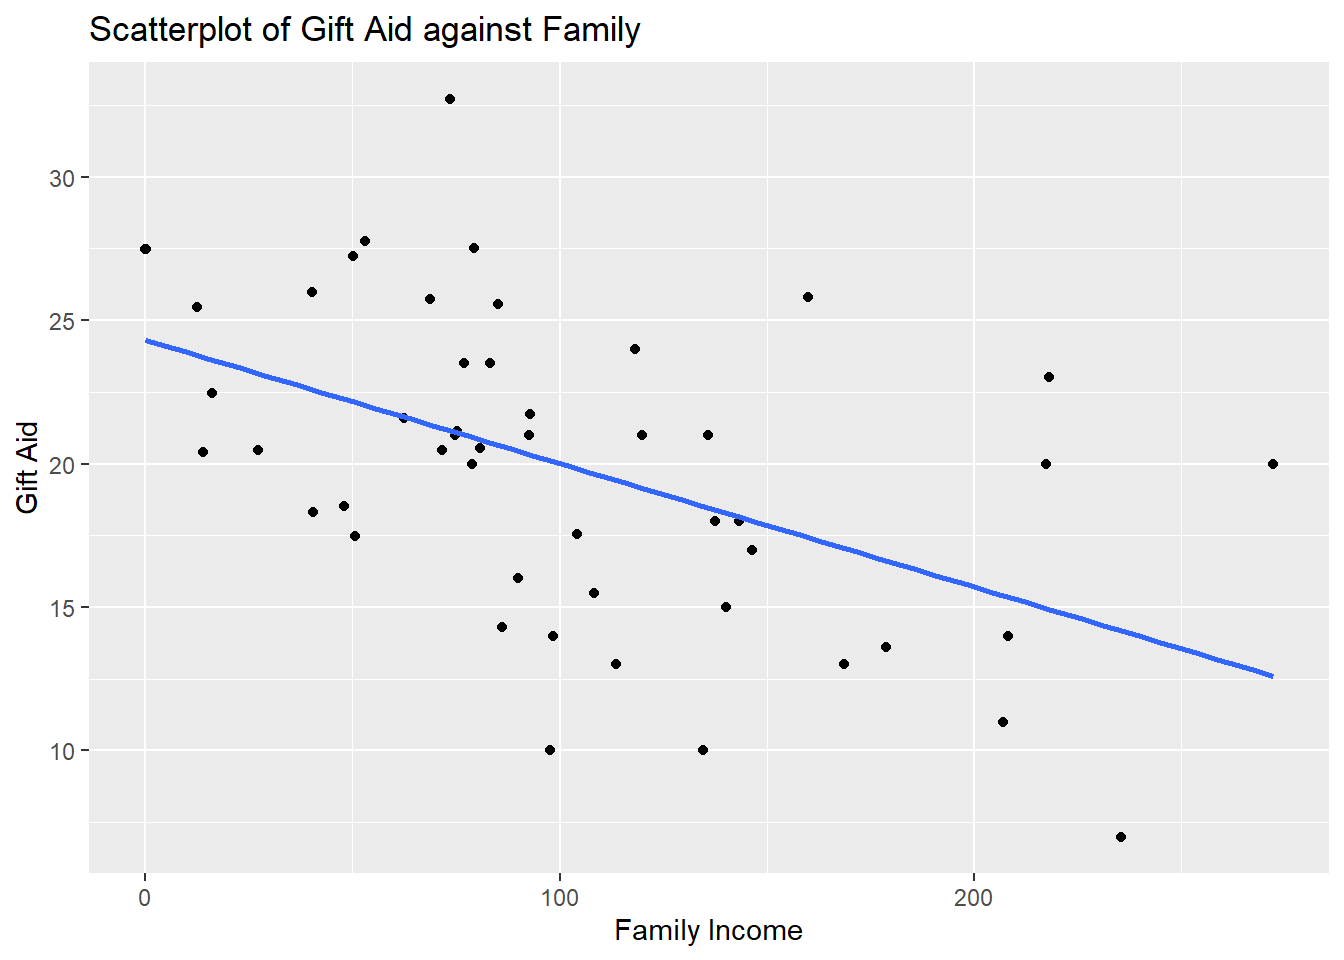
\includegraphics{bookdown-demo_files/figure-latex/unnamed-chunk-120-1.pdf}

We note that the observations are fairly evenly scattered on both sides of the regression line, so a linear association exists. We see a negative linear association. As family income increases, the gift aid, on average, decreases.

We also do not see any observation with weird values that may warrant further investigation.

\hypertarget{regression}{%
\subsection*{Regression}\label{regression}}
\addcontentsline{toc}{subsection}{Regression}

We use the \texttt{lm()} function to fit a regression model:

\begin{Shaded}
\begin{Highlighting}[]
\DocumentationTok{\#\#regress gift aid against family income}
\NormalTok{result}\OtherTok{\textless{}{-}}\FunctionTok{lm}\NormalTok{(gift\_aid}\SpecialCharTok{\textasciitilde{}}\NormalTok{family\_income, }\AttributeTok{data=}\NormalTok{Data)}
\end{Highlighting}
\end{Shaded}

Use the \texttt{summary()} function to display relevant information from this regression:

\begin{Shaded}
\begin{Highlighting}[]
\DocumentationTok{\#\#look at information regarding regression}
\FunctionTok{summary}\NormalTok{(result)}
\end{Highlighting}
\end{Shaded}

\begin{verbatim}
## 
## Call:
## lm(formula = gift_aid ~ family_income, data = Data)
## 
## Residuals:
##      Min       1Q   Median       3Q      Max 
## -10.1128  -3.6234  -0.2161   3.1587  11.5707 
## 
## Coefficients:
##               Estimate Std. Error t value Pr(>|t|)    
## (Intercept)   24.31933    1.29145  18.831  < 2e-16 ***
## family_income -0.04307    0.01081  -3.985 0.000229 ***
## ---
## Signif. codes:  0 '***' 0.001 '**' 0.01 '*' 0.05 '.' 0.1 ' ' 1
## 
## Residual standard error: 4.783 on 48 degrees of freedom
## Multiple R-squared:  0.2486, Adjusted R-squared:  0.2329 
## F-statistic: 15.88 on 1 and 48 DF,  p-value: 0.0002289
\end{verbatim}

We see the following values:

\begin{itemize}
\tightlist
\item
  \(\hat{\beta}_1 =\) -0.0430717. The estimated slope informs us the the predicted gift aid decreases by 0.0430717 thousands of dollars (or \$43.07) per unit increase in family income.
\item
  \(\hat{\beta}_0 =\) 24.319329. For students with no family income, their predicted gift aid is \$24 319.33. Note: from the scatterplot, we have an observation with 0 family income. We must be careful in not extrapolating when making predictions with our regression. We should only make predictions for family incomes between the minimum and maximum values of family incomes in our data.
\item
  \(s\) = 4.7825989, is the estimate of the standard deviation of the error terms. This is reported as residual standard error in R. Squaring this gives the estimated variance.
\item
  \(F\) = 15.8772043. This is the value of the ANOVA \(F\) statistic. The corresponding p-value is reported. Since this p-value is very small, we reject the null hypothesis. The data support the claim that there is a linear association between gift aid and family income.
\item
  \(R^2 =\) 0.2485582. The coefficient of determination informs us that about 24.86\% of the variation in gift aid can be explained by family income.
\end{itemize}

\hypertarget{extract-values-from-r-objects}{%
\subsubsection*{Extract values from R objects}\label{extract-values-from-r-objects}}
\addcontentsline{toc}{subsubsection}{Extract values from R objects}

We can actually extract these values that are being reported from \texttt{summary(result)}. To see what can be extracted from an R object, use the \texttt{names()} function:

\begin{Shaded}
\begin{Highlighting}[]
\DocumentationTok{\#\#see what can be extracted from summary(result)}
\FunctionTok{names}\NormalTok{(}\FunctionTok{summary}\NormalTok{(result))}
\end{Highlighting}
\end{Shaded}

\begin{verbatim}
##  [1] "call"          "terms"         "residuals"     "coefficients" 
##  [5] "aliased"       "sigma"         "df"            "r.squared"    
##  [9] "adj.r.squared" "fstatistic"    "cov.unscaled"
\end{verbatim}

To extract the estimated coefficients:

\begin{Shaded}
\begin{Highlighting}[]
\DocumentationTok{\#\#extract coefficients}
\FunctionTok{summary}\NormalTok{(result)}\SpecialCharTok{$}\NormalTok{coefficients}
\end{Highlighting}
\end{Shaded}

\begin{verbatim}
##                  Estimate Std. Error   t value     Pr(>|t|)
## (Intercept)   24.31932901 1.29145027 18.831022 8.281020e-24
## family_income -0.04307165 0.01080947 -3.984621 2.288734e-04
\end{verbatim}

Notice the information is presented in a table. To extract a specific value, we can specify the row and column indices:

\begin{Shaded}
\begin{Highlighting}[]
\DocumentationTok{\#\#extract slope}
\FunctionTok{summary}\NormalTok{(result)}\SpecialCharTok{$}\NormalTok{coefficients[}\DecValTok{2}\NormalTok{,}\DecValTok{1}\NormalTok{]}
\end{Highlighting}
\end{Shaded}

\begin{verbatim}
## [1] -0.04307165
\end{verbatim}

\begin{Shaded}
\begin{Highlighting}[]
\DocumentationTok{\#\#extract intercept}
\FunctionTok{summary}\NormalTok{(result)}\SpecialCharTok{$}\NormalTok{coefficients[}\DecValTok{1}\NormalTok{,}\DecValTok{1}\NormalTok{]}
\end{Highlighting}
\end{Shaded}

\begin{verbatim}
## [1] 24.31933
\end{verbatim}

On your own, extract the values of the residual standard error, the ANOVA F statistic, and \(R^2\).

\hypertarget{prediction}{%
\subsubsection*{Prediction}\label{prediction}}
\addcontentsline{toc}{subsubsection}{Prediction}

A use of regression models is prediction. Suppose I want to predict the gift aid of a student with family income of 50 thousand dollars (assuming the unit is in thousands of dollars). We use the \texttt{predict()} function:

\begin{Shaded}
\begin{Highlighting}[]
\DocumentationTok{\#\#create data point for prediction}
\NormalTok{newdata}\OtherTok{\textless{}{-}}\FunctionTok{data.frame}\NormalTok{(}\AttributeTok{family\_income=}\DecValTok{50}\NormalTok{)}
\DocumentationTok{\#\#predicted gift aid when x=50}
\FunctionTok{predict}\NormalTok{(result,newdata)}
\end{Highlighting}
\end{Shaded}

\begin{verbatim}
##        1 
## 22.16575
\end{verbatim}

This student's predicted gift aid is \$22 165.75. Alternatively, you could have calculated this by plugging \(x=50\) into the estimated SLR equation:

\begin{Shaded}
\begin{Highlighting}[]
\FunctionTok{summary}\NormalTok{(result)}\SpecialCharTok{$}\NormalTok{coefficients[}\DecValTok{1}\NormalTok{,}\DecValTok{1}\NormalTok{] }\SpecialCharTok{+} \FunctionTok{summary}\NormalTok{(result)}\SpecialCharTok{$}\NormalTok{coefficients[}\DecValTok{2}\NormalTok{,}\DecValTok{1}\NormalTok{]}\SpecialCharTok{*}\DecValTok{50}
\end{Highlighting}
\end{Shaded}

\begin{verbatim}
## [1] 22.16575
\end{verbatim}

\hypertarget{anova-table-1}{%
\subsubsection*{ANOVA table}\label{anova-table-1}}
\addcontentsline{toc}{subsubsection}{ANOVA table}

We use the \texttt{anova()} function to display the ANOVA table

\begin{Shaded}
\begin{Highlighting}[]
\NormalTok{anova.tab}\OtherTok{\textless{}{-}}\FunctionTok{anova}\NormalTok{(result)}
\NormalTok{anova.tab}
\end{Highlighting}
\end{Shaded}

\begin{verbatim}
## Analysis of Variance Table
## 
## Response: gift_aid
##               Df  Sum Sq Mean Sq F value    Pr(>F)    
## family_income  1  363.16  363.16  15.877 0.0002289 ***
## Residuals     48 1097.92   22.87                      
## ---
## Signif. codes:  0 '***' 0.001 '**' 0.01 '*' 0.05 '.' 0.1 ' ' 1
\end{verbatim}

The report \(F\) statistic is the same as the value reported earlier from \texttt{summary(result)}.

The first line of the output gives \(SS_{R}\), the second line gives \(SS_{res}\). The function doesn't provide \(SS_T\), but we know that \(SS_T = SS_{R} + SS_{res}\).

Again, to see what can be extracted from \texttt{anova.tab}:

\begin{Shaded}
\begin{Highlighting}[]
\FunctionTok{names}\NormalTok{(anova.tab)}
\end{Highlighting}
\end{Shaded}

\begin{verbatim}
## [1] "Df"      "Sum Sq"  "Mean Sq" "F value" "Pr(>F)"
\end{verbatim}

So \(SS_T\) can be easily calculated:

\begin{Shaded}
\begin{Highlighting}[]
\NormalTok{SST}\OtherTok{\textless{}{-}}\FunctionTok{sum}\NormalTok{(anova.tab}\SpecialCharTok{$}\StringTok{"Sum Sq"}\NormalTok{)}
\NormalTok{SST}
\end{Highlighting}
\end{Shaded}

\begin{verbatim}
## [1] 1461.079
\end{verbatim}

The \(R^2\) was reported to be 0.2485582. To verify using the ANOVA table:

\begin{Shaded}
\begin{Highlighting}[]
\NormalTok{anova.tab}\SpecialCharTok{$}\StringTok{"Sum Sq"}\NormalTok{[}\DecValTok{1}\NormalTok{]}\SpecialCharTok{/}\NormalTok{SST}
\end{Highlighting}
\end{Shaded}

\begin{verbatim}
## [1] 0.2485582
\end{verbatim}

\hypertarget{correlation-1}{%
\subsection*{Correlation}\label{correlation-1}}
\addcontentsline{toc}{subsection}{Correlation}

We use the \texttt{cor()} function to find the correlation between two quantitative variables:

\begin{Shaded}
\begin{Highlighting}[]
\DocumentationTok{\#\#correlation}
\FunctionTok{cor}\NormalTok{(Data}\SpecialCharTok{$}\NormalTok{family\_income,Data}\SpecialCharTok{$}\NormalTok{gift\_aid)}
\end{Highlighting}
\end{Shaded}

\begin{verbatim}
## [1] -0.4985561
\end{verbatim}

The correlation is -0.4985561. We have a moderate, negative linear association between family income and gift aid.

\hypertarget{inf}{%
\chapter{Inference with Simple Linear Regression (SLR)}\label{inf}}

\hypertarget{introduction-3}{%
\section{Introduction}\label{introduction-3}}

Oftentimes, the data we collect come from a random sample that is representative of the population of interest. A common example is an election poll before a presidential election. Random sampling allows the sample to be representative of the population. However, if we obtain another random sample, the characteristics of the new sample are unlikely to be exactly the same as the first sample. For example, the sample proportion who will vote for a certain party is unlikely to be the same for both random samples. What this tells us is that even with representative samples, sample proportions are unlikely to be equal to the population proportion, and sample proportions vary from sample to sample.

Dr.~W. Edwards Deming's Red Bead experiment illustrates this concept. A video of this experiment \href{https://www.youtube.com/watch?v=R3ewHrpqclA}{can be found here.}

In this video, the number of red beads, which represent bad products, varies each time the worker obtains a random sample of 50 beads. The fact that the number of red beads increases in his second sample does not indicate that he performed his task any worse, as this increase is due to the random variation associated with samples.

Note: Deming's Red Bead experiment was developed to illustrate concepts associated with management. He is best known for his work in developing the Japanese economy after World War II. You will be able to find many blogs/articles discussing the experiment on the World Wide Web. Although many of the articles discuss how this experiment applies in management, it can be used to illustrate concepts of variation.

The same idea extends to the slope and intercept of a regression line. The estimated slope and intercept will vary from sample to sample and are unlikely to be equal to the population slope and intercept. In inferential statistics, we use hypothesis tests and confidence intervals to aid us in accounting for this random variation. In this module, you will learn how to account for and quantify the random variation associated with the estimated regression model, and how to interpret the estimated regression model while accounting for random variation.

\hypertarget{review-from-previous-module}{%
\subsection{Review from previous module}\label{review-from-previous-module}}

The \textbf{simple linear regression model} is written as

\begin{equation}
y=\beta_0+\beta_{1} x + \epsilon. 
\label{eq:4SLRmod}
\end{equation}

We make some assumptions for the error term \(\epsilon\). They are:

\begin{enumerate}
\def\labelenumi{\arabic{enumi}.}
\tightlist
\item
  The errors have mean 0.
\item
  The \textbf{errors have variance denoted by \(\sigma^2\)}. Notice this variance is constant.
\item
  The errors are independent.
\item
  The errors are normally distributed.
\end{enumerate}

These assumptions allow us to derive the distributional properties associated with our least squares estimators \(\hat{\beta}_0, \hat{\beta}_1\), which then enables us to compute reliable confidence intervals and perform hypothesis tests on our SLR reliably.

\(\hat{\beta}_1,\hat{\beta}_0\) are the estimators for \(\beta_1,\beta_0\) respectively. These estimators can be interpreted in the following manner:

\begin{itemize}
\tightlist
\item
  \textbf{\(\hat{\beta}_1\) denotes the change in the predicted \(y\) when \(x\) increases by 1 unit. Alternatively, it denotes the change in \(y\), on average, when \(x\) increases by 1 unit.}
\item
  \textbf{\(\hat{\beta}_0\) denotes the predicted \(y\) when \(x=0\). Alternatively, it denotes the average of \(y\) when \(x=0\).}
\end{itemize}

How do the values of these estimators vary from sample to sample?

\hypertarget{hypothesis-testing-in-slr}{%
\section{Hypothesis Testing in SLR}\label{hypothesis-testing-in-slr}}

\hypertarget{distribution-of-least-squares-estimators}{%
\subsection{Distribution of least squares estimators}\label{distribution-of-least-squares-estimators}}

\textbf{Gauss Markov Theorem}: Under assumptions for a regression model, the least squares estimators \(\hat{\beta}_1\) and \(\hat{\beta}_0\) are unbiased and have minimum variance among all unbiased linear estimators.

Thus, the least squares estimators have the following properties:

\begin{enumerate}
\def\labelenumi{\arabic{enumi}.}
\tightlist
\item
  \(\mbox{E}(\hat{\beta}_1) = \beta_1\), \(\mbox{E}(\hat{\beta}_0) = \beta_0\)
\end{enumerate}

Note: An estimator is \textbf{unbiased} if its expected value is exactly equal to the parameter it is estimating.

\begin{enumerate}
\def\labelenumi{\arabic{enumi}.}
\setcounter{enumi}{1}
\tightlist
\item
  The variance of \(\hat{\beta}_1\) is
\end{enumerate}

\begin{equation} 
\mbox{Var}(\hat{\beta}_1) = \frac{\sigma^{2}}{\sum{(x_{i}-\bar{x})^{2}}}
\label{eq:4varb1}
\end{equation}

\begin{enumerate}
\def\labelenumi{\arabic{enumi}.}
\setcounter{enumi}{2}
\tightlist
\item
  The variance of \(\hat{\beta}_0\) is
\end{enumerate}

\begin{equation} 
\mbox{Var}(\hat{\beta}_0) = \sigma^2 \left[\frac{1}{n} + \frac{\bar{x}^2}{\sum (x_i -\bar{x})^2}\right]
\label{eq:4varb0}
\end{equation}

\begin{enumerate}
\def\labelenumi{\arabic{enumi}.}
\setcounter{enumi}{3}
\tightlist
\item
  \(\hat{\beta}_1\) and \(\hat{\beta}_0\) both follow a normal distribution.
\end{enumerate}

Note that in \eqref{eq:4varb1} and \eqref{eq:4varb0}, we use \(s^2 = MS_{res}\) to estimate \(\sigma^2\) since \(\sigma^2\) is a unknown value.

What these imply is that if we standardize \(\hat{\beta}_1\) and \(\hat{\beta}_0\), these standardized quantities will follow a \(t_{n-2}\) distribution, i.e.

\begin{equation} 
\frac{\hat{\beta}_1 - \beta_1}{se(\hat{\beta}_1)}\sim t_{n-2}
\label{eq:distb1}
\end{equation}

and

\begin{equation} 
\frac{\hat{\beta}_0 - \beta_0}{se(\hat{\beta}_0)}\sim t_{n-2},
\label{eq:distb0}
\end{equation}

where

\begin{equation}
se(\hat{\beta}_1) = \sqrt{\frac{MS_{res}}{\sum{(x_{i}-\bar{x})^{2}}}} = \frac{s}{\sqrt{\sum{(x_{i}-\bar{x})^{2}}}}
\label{eq:seb1}
\end{equation}

and

\begin{equation} 
se(\hat{\beta}_0) = \sqrt{MS_{res}\left[\frac{1}{n} + \frac{\bar{x}^2}{\sum (x_i -\bar{x})^2}\right]} = s \sqrt{\frac{1}{n} + \frac{\bar{x}^2}{\sum (x_i -\bar{x})^2}}
\label{eq:seb0}
\end{equation}

Note:

\begin{itemize}
\item
  \(se(\hat{\beta}_1)\) is read as the \textbf{standard error of \(\hat{\beta}_1\)}. The standard error of any estimator is essentially the sample standard deviation of that estimator, and measures the spread of that estimator.
\item
  A \(t_{n-2}\) distribution is read as a \textbf{\(t\) distribution with \(n-2\) degrees of freedom}.
\end{itemize}

\hypertarget{testing-regression-coefficients}{%
\subsection{Testing regression coefficients}\label{testing-regression-coefficients}}

Hypothesis testing is used to investigate if a population parameter is \textbf{different from a specific value}. In the context of SLR, we usually want to test if \(\beta_1\) is 0 or not. If \(\beta_1 = 0\), there is no linear relationship between the variables.

The general steps in hypothesis testing are:

\begin{itemize}
\tightlist
\item
  Step 1: State the null and alternative hypotheses.
\item
  Step 2: A test statistic is calculated using the sample, assuming the null is true. The value of the test statistic measures how the \textbf{sample deviates from the null}.
\item
  Step 3: Make conclusion, using either critical values or p-values.
\end{itemize}

In the previous module, we introduced the ANOVA \(F\) test. In SLR, this tests if the slope of the SLR equation is 0 or not. It turns out that we can also perform a \(t\) test for the slope. In the \(t\) test for the slope, the null and alternative hypotheses are:

\[
H_0: \beta_1 = 0, H_a: \beta_1 \neq 0.
\]
The test statistic is

\begin{equation} 
t = \frac{\hat{\beta}_1 - \text{ value in null}}{se(\hat{\beta}_1)}
\label{eq:4ttest}
\end{equation}

which is compared with a \(t_{n-2}\) distribution. Notice that \eqref{eq:4ttest} comes from \eqref{eq:distb1}.

Let us go back to our simulated example that we saw in the last module. We have data from 6000 UVa undergraduate students on the amount of time they spend studying in a week (in minutes), and how many courses they are taking in the semester (3 or 4 credit courses).

\begin{Shaded}
\begin{Highlighting}[]
\DocumentationTok{\#\#create dataframe}
\NormalTok{df}\OtherTok{\textless{}{-}}\FunctionTok{data.frame}\NormalTok{(study,courses)}

\DocumentationTok{\#\#fit regression}
\NormalTok{result}\OtherTok{\textless{}{-}}\FunctionTok{lm}\NormalTok{(study}\SpecialCharTok{\textasciitilde{}}\NormalTok{courses, }\AttributeTok{data=}\NormalTok{df)}
\DocumentationTok{\#\#look at regression coefficients}
\FunctionTok{summary}\NormalTok{(result)}\SpecialCharTok{$}\NormalTok{coefficients}
\end{Highlighting}
\end{Shaded}

\begin{verbatim}
##              Estimate Std. Error   t value      Pr(>|t|)
## (Intercept)  58.44829  1.9218752  30.41211 4.652442e-189
## courses     120.39310  0.4707614 255.74125  0.000000e+00
\end{verbatim}

The \(t\) statistic for testing \(H_0: \beta_1 = 0, H_a: \beta_1 \neq 0\) is reported to be 255.7412482, which can be calculated using \eqref{eq:4ttest}: \(t= \frac{120.39310 - 0}{0.4707614}\). The reported p-value is virtually 0, so we reject the null hypothesis. The data support the claim that there is a linear association between study time and the number of courses taken.

\hypertarget{confidence-intervals-for-regression-coefficients}{%
\section{Confidence Intervals for Regression Coefficients}\label{confidence-intervals-for-regression-coefficients}}

Confidence intervals (CIs) are similar to hypothesis testing in the sense that they are also based on the distributional properties of an estimator. CIs may differ in their use in the following ways:

\begin{enumerate}
\def\labelenumi{\arabic{enumi}.}
\tightlist
\item
  We are not assessing if the parameter is different from a specific value.
\item
  We are more interested in exploring a plausible \textbf{range of values for an unknown parameter}.
\end{enumerate}

Because CIs and hypothesis tests are based on the distributional properties of an estimator, their conclusions will be consistent (as long as the significance level is the same).

Recall the general form for CIs:

\begin{equation} 
\mbox{estimator} \pm (\mbox{multiplier} \times \mbox{s.e of estimator}). 
\label{eq:4CI}
\end{equation}

We have the following components of a CI

\begin{itemize}
\tightlist
\item
  \textbf{estimator (or statistic)}: numerical quantity that describes a sample
\item
  \textbf{multiplier}: determined by confidence level and relevant probability distribution
\item
  \textbf{standard error of estimator}: measure of variance of estimator (basically the square root of the variance of estimator)
\end{itemize}

Following \eqref{eq:4CI} and \eqref{eq:distb1}, the \(100(1-\alpha)\%\) CI for \(\beta_1\) is

\begin{equation} 
\hat{\beta}_1 \pm t_{1-\alpha/2;n-2}  se(\hat{\beta}_1) = \hat{\beta}_1 \pm t_{1-\alpha/2;n-2} \frac{s}{\sqrt{\sum(x_i - \bar{x})^{2}}}.
\label{eq:4CIb1}
\end{equation}

Going back to our study time example, the 95\% CI for \(\beta_1\) is (119.470237, 121.3159601).

\begin{Shaded}
\begin{Highlighting}[]
\DocumentationTok{\#\#CI for coefficients}
\FunctionTok{confint}\NormalTok{(result,}\AttributeTok{level =} \FloatTok{0.95}\NormalTok{)[}\DecValTok{2}\NormalTok{,]}
\end{Highlighting}
\end{Shaded}

\begin{verbatim}
##    2.5 %   97.5 % 
## 119.4702 121.3160
\end{verbatim}

An interpretation of this CI is that we have 95\% confidence that the true slope \(\beta_1\) lies between (119.470237, 121.3159601). In other words, for each additional course taken, the predicted study time increases between 119.470237 and 121.3159601 minutes.

\hypertarget{thought-questions}{%
\subsection{Thought questions}\label{thought-questions}}

\begin{itemize}
\item
  Is the conclusion from this 95\% CI consistent with the hypothesis test for \(H_0: \beta_1 = 0\) in the previous section at 0.05 significance level?
\item
  I have presented hypothesis tests and CIs for the slope, \(\beta_1\).

  \begin{itemize}
  \item
    How would you calculate the \(t\) statistic if you wanted to test \(H_0: \beta_0 = 0, H_0: \beta_0 \neq 0\)?
  \item
    How would you calculate the 95\% CI for the intercept \(\beta_0\)?
  \end{itemize}
\end{itemize}

Generally, we are usually more interested in the slope than the intercept.

\hypertarget{ci-of-the-mean-response}{%
\section{CI of the Mean Response}\label{ci-of-the-mean-response}}

We have established that the least squares estimators \(\hat{\beta}_1,\hat{\beta}_0\) have their associated variances. Since the estimated SLR equation is

\begin{equation} 
\hat{y}=\hat{\beta}_0+\hat{\beta}_1 x,
\label{eq:4fitted}
\end{equation}

it stands to reason that \(\hat{y}\) has an associated variance as well, since it is a function of \(\hat{\beta}_1,\hat{\beta}_0\).

There are two interpretations of \(\hat{y}\):

\begin{enumerate}
\def\labelenumi{\arabic{enumi}.}
\tightlist
\item
  it \textbf{estimates the mean of \(y\) when \(x=x_0\)};
\item
  it \textbf{predicts the value of \(y\) for a new observation when \(x=x_0\)}.
\end{enumerate}

Note: \(x_0\) denotes a specific numerical value for the predictor variable.

Depending on which interpretation we want, there are two different intervals based on \(\hat{y}\). The first interpretation is associated with the \textbf{confidence interval for the mean response, \(\hat{\mu}_{y|x_0}\), given the predictor}. This is used when we are interested in the average value of the response variable, when the predictor is equal to a specific value. This CI is

\begin{equation} 
\hat{\mu}_{y|x_0}\pm t_{1-\alpha/2,n-2}s\sqrt{\frac{1}{n} +
\frac{(x_0-\bar{x})^2}{\sum(x_i-\bar{x})^2}}.
\label{eq:4CImean}
\end{equation}

Going back to our study time example, suppose we want the average study time for students who take 5 courses, the 95\% CI is

\begin{Shaded}
\begin{Highlighting}[]
\DocumentationTok{\#\#CI for mean y when x=5}
\NormalTok{newdata}\OtherTok{\textless{}{-}}\FunctionTok{data.frame}\NormalTok{(}\AttributeTok{courses=}\DecValTok{5}\NormalTok{)}
\FunctionTok{predict}\NormalTok{(result, newdata, }\AttributeTok{level=}\FloatTok{0.95}\NormalTok{, }\AttributeTok{interval=}\StringTok{"confidence"}\NormalTok{)}
\end{Highlighting}
\end{Shaded}

\begin{verbatim}
##        fit      lwr      upr
## 1 660.4138 659.2224 661.6052
\end{verbatim}

We have 95\% confidence that the average study time for students who take 5 courses is between 659.2223688 and 661.605187 minutes.

\hypertarget{pi-of-a-new-response}{%
\section{PI of a New Response}\label{pi-of-a-new-response}}

Previously, we found a CI for the mean of \(y\) given a specific value of \(x\), \eqref{eq:4CImean}. This CI gives us an idea about the location of the regression line at a specific of \(x\).

Instead, we may have interest in finding an interval for a new value of \(\hat{y}_0\), when we have a new observation \(x=x_0\). This is called a \textbf{prediction interval (PI) for a future observation \(y_0\) when the predictor is a specific value}. This interval follows from the second interpretation of \(\hat{y}\).

The PI for \(\hat{y}_0\) takes into account:

\begin{enumerate}
\def\labelenumi{\arabic{enumi}.}
\tightlist
\item
  Variation in location for the distribution of \(y\) (i.e.~where is the center of the distribution of \(y\)?).
\item
  Variation \textbf{within the probability distribution of \(y\)}.
\end{enumerate}

By comparison, the confidence interval for the mean response \eqref{eq:4CImean} only takes into account the first element. The PI is

\begin{equation} 
\hat{y}_0\pm t_{1-\alpha/2,n-2}s \sqrt{1+\frac{1}{n} +
\frac{(x_0-\bar{x})^2}{\sum(x_i-\bar{x})^2}}.
\label{eq:4pred}
\end{equation}

Going back to our study time example, suppose we have a newly enrolled student who wishes to take 5 courses, and the student wants to predict his study time

\begin{Shaded}
\begin{Highlighting}[]
\DocumentationTok{\#\#PI for y when x=5}
\FunctionTok{predict}\NormalTok{(result, newdata, }\AttributeTok{level=}\FloatTok{0.95}\NormalTok{, }\AttributeTok{interval=}\StringTok{"prediction"}\NormalTok{)}
\end{Highlighting}
\end{Shaded}

\begin{verbatim}
##        fit      lwr      upr
## 1 660.4138 602.0347 718.7928
\end{verbatim}

We have 95\% confidence that the study time for this student is between 602.0347305 and 718.7928253 minutes.

\hypertarget{thought-questions-1}{%
\subsection{Thought questions}\label{thought-questions-1}}

\begin{itemize}
\item
  In the following two scenarios, decide if we are more interested in the CI for the mean response given the predictor \eqref{eq:4CImean}, or the PI for a future response given the predictor \eqref{eq:4pred}.

  \begin{itemize}
  \item
    We wish to estimate the waiting time, on average, of DMV customers if there are 10 people in line at the DMV.
  \item
    I enter the DMV and notice 10 people in line. I want to estimate my waiting time.
  \end{itemize}
\item
  Look at the standard errors associated with the intervals given in \eqref{eq:4CImean} and \eqref{eq:4pred}. How are they related to each other?
\end{itemize}

\hypertarget{supplemental-notes-on-statistical-inference}{%
\section{Supplemental Notes on Statistical Inference}\label{supplemental-notes-on-statistical-inference}}

\hypertarget{hypothesis-statements}{%
\subsection{Hypothesis statements}\label{hypothesis-statements}}

Let's consider a \(t\) test for the regression parameter, \(\beta_1\). Depending on context, the following could be null and alternative hypotheses

\begin{itemize}
\tightlist
\item
  \(H_0: \beta_1 = 0, H_a: \beta_1 \neq 0\).
\item
  \(H_0: \beta_1 = 0, H_a: \beta_1 > 0\).
\item
  \(H_0: \beta_1 = 0, H_a: \beta_1 < 0\).
\end{itemize}

The null hypothesis should be stated as a statement of \textbf{equality}. This concept holds true for hypothesis tests in general. Some other books / resources might state them as

\begin{itemize}
\tightlist
\item
  \(H_0: \beta_1 = 0, H_a: \beta_1 \neq 0\).
\item
  \(H_0: \beta_1 \leq 0, H_a: \beta_1 > 0\).
\item
  \(H_0: \beta_1 \geq 0, H_a: \beta_1 < 0\).
\end{itemize}

I prefer using the equality statement for the null hypothesis for the following reasons (theoretical, pedagogical, practical):

\begin{enumerate}
\def\labelenumi{\arabic{enumi}.}
\tightlist
\item
  The null hypothesis being an equality aligns with the definition of the p-value.
\end{enumerate}

\begin{itemize}
\tightlist
\item
  The p-value is the probability of observing our sample estimate (or a value more extreme), if the null hypothesis is true (i.e.~\(\beta_1\) is truly 0). This is what we are assuming in the calculation for the test statistic.
\end{itemize}

\begin{enumerate}
\def\labelenumi{\arabic{enumi}.}
\setcounter{enumi}{1}
\tightlist
\item
  People tend to get confused between the null and alternative hypotheses if both involve inequalities (the alternative is the hypothesis you are trying to support).
\item
  Conclusions are made in terms of supporting (or not supporting) the alternative hypothesis.
\end{enumerate}

\hypertarget{sample-size-and-statistical-inference}{%
\subsection{Sample size and statistical inference}\label{sample-size-and-statistical-inference}}

Generally speaking, there is a relationship between sample size and statistical inference (assuming other characteristics remain the same and our sample was randomly obtained or representative of the population of interest):

\begin{itemize}
\tightlist
\item
  Larger sample sizes (typically) lead to narrower confidence intervals (more precise intervals).
\item
  Sample estimates based on larger samples are more likely to be closer to the true parameters.
\item
  Larger sample (typically) lead to more evidence against the null hypothesis.

  \begin{itemize}
  \tightlist
  \item
    This means a larger sample size leads to a more powerful test. The power of a test is the probability a hypothesis test is able to correctly reject the null hypothesis.
  \end{itemize}
\end{itemize}

\hypertarget{small-sample-sizes}{%
\subsubsection{Small sample sizes}\label{small-sample-sizes}}

Small sample sizes tend to result in:

\begin{itemize}
\tightlist
\item
  Confidence intervals that are wide.
\item
  Sample estimates that are more likely to be further away from the true parameters.
\item
  Hypothesis tests that are more likely to incorrectly fail to reject the null hypothesis when the alternative hypothesis is true.
\end{itemize}

While larger sample sizes have their advantages, there are also some disadvantages with sample sizes that are extremely large.

\hypertarget{large-sample-sizes}{%
\subsubsection{Large sample sizes}\label{large-sample-sizes}}

A ``statistically significant'' result does not necessarily mean that the result has practical consequences. Suppose a 95\% confidence interval for \(\beta_1\) is \((0.001, 0.002)\). The interval excludes 0, so it is ``statistically significantly'' different from 0 (because it is!), but does this result have practical consequences? A narrow CI that barely excludes the null value can happen when we have a large sample size.

If one was to conduct the corresponding hypothesis test, we would reject the null hypothesis that \(\beta_1 = 0\). With large sample sizes, hypothesis tests are sensitive to small departures from the null hypothesis.

In such instances, it may be worth considering hypothesis tests involving a different value in the null hypothesis, one that makes sense for your question. For example, a practically significant slope may need to be greater than a specific numerical value for a certain context.

\begin{itemize}
\tightlist
\item
  Statistical inference to assess statistical significance.
\item
  Subject area knowledge to assess practical significance.
\end{itemize}

\hypertarget{questions}{%
\subsubsection{Questions}\label{questions}}

Are the following results statistically significant? If so, are the results also practically significant? Assume a two-sided test with a null value of 0 (These are made up examples):

\begin{enumerate}
\def\labelenumi{\arabic{enumi}.}
\item
  In assessing if studying more is associated with better test scores, a SLR is carried out with test scores (out of 100 points) against study time (in hours). The 95\% confidence interval for the slope \(\beta_1\) is (5.632, 7.829).
\item
  A SLR is carried out to explore the linear relationship between number of years in school with income (in thousands of dollars). The 95\% confidence interval for the slope \(\beta_1\) is (0.051, 0.243).
\end{enumerate}

\hypertarget{cautions-using-slr-and-correlation}{%
\subsection{Cautions using SLR and Correlation}\label{cautions-using-slr-and-correlation}}

Simple linear regression and correlation are meant for assessing \textbf{linear} relationships. If the relationship is not linear, we will need to transform the variable(s) (so the transformed variables have a linear relationship. Will explore this in Module \ref{diag}).

\begin{itemize}
\tightlist
\item
  Always verify via a scatterplot that the relationship is at least approximately linear.
\item
  A high correlation or a significant estimated slope by themselves do not prove that we have a strong linear relationship between the variables. Conversely, a correlation close to 0 or an insignificant estimated slope is also not proof that we do not have a relationship between the variables.
\end{itemize}

\hypertarget{outliers}{%
\subsubsection{Outliers}\label{outliers}}

SLR and correlation are sensitive to outliers / influential observations. Generally speaking, these are data that are ``far away'' or very different from the rest of the observations. These data points can be visually inspected from a scatterplot. Some potential considerations when dealing with such data points:

\begin{itemize}
\tightlist
\item
  Investigate these observations. There is usually something that is making them ``stand out'' from the rest of the data.
\item
  Data entry errors that can be corrected. Be sure to mention in the report.
\item
  Revisit how the data were sampled. Perhaps the data point is is not part of the population of interest. If so, data point can be removed (this is legitimate), but be sure to mention in the report.
\end{itemize}

With regards to regression analysis:

\begin{itemize}
\tightlist
\item
  Exclusion of data points must be clearly documented.
\item
  Fit the regression with and without the data points in question, and see how similar or different the conclusions become.
\item
  If the data points have large value(s) on the predictor and/or response, a log transformation on the variable can pull in the large values.
\item
  Consider subsetting your data and create separate models for each subset; or focus on a subset and make it clear your analysis is for a subset.
\item
  Knowing your data and context can help a lot in these decisions.
\end{itemize}

\hypertarget{association-and-causation}{%
\subsubsection{Association and causation}\label{association-and-causation}}

Two correlated variables do not mean that one variable causes the other variable to change. For example, consider a plot of ice cream consumption and deaths by drowning during various months. There may be some positive correlation, and clearly, eating more ice cream does not cause more drownings. The correlation can be explained by a third (lurking) variable: the weather.

A \textbf{lurking variable} is a variable that has an impact on the relationship between the variables being studied, but is itself not studied.

A carefully designed \textbf{randomized experiment} can control for lurking variables, and causal relationships can be established. Typically, such experiments include:

\begin{itemize}
\tightlist
\item
  A control group and a treatment group.
\item
  Random assignment of large number of observations into the treatment and control groups. Due to the random assignment, the general characteristics of of subjects in each group are similar.
\end{itemize}

Lurking variables are always an issue with \textbf{observational studies}. Researchers in observational studies do not intervene with the observations and simply observe the data that the observations generate. Causal relationships are much more difficult to establish with observational studies.

\hypertarget{questions-1}{%
\subsubsection{Questions}\label{questions-1}}

\begin{enumerate}
\def\labelenumi{\arabic{enumi}.}
\item
  Consider the \texttt{palmerpenguins} dataset that we have been working on. The data contain size measurements for three different species of penguins on three islands in the Palmer Archipelago, Antarctica over three years. Is this an observational study or randomized experiment?
\item
  A fertilizer company wishes to evaluate how effective a new fertilizer is in terms of improving the yield of crops. A large field is divided into many smaller plots, and each smaller plot is randomly assigned to receive either the new fertilizer or the standard fertilizer. Is this an observational study or randomized experiment?
\item
  A professor wishes to evaluate the effectiveness of various teaching methods (traditional vs flipped classroom). The professor uses the traditional approach for a section that meets on Mondays, Wednesdays, and Fridays from 9 to 10am and uses the flipped classroom approach for a section that meets on Mondays, Wednesdays, and Fridays from 2 to 3pm. Students were free to choose whichever section that wanted to register for, with no knowledge of the teaching method being used. What are some potential lurking variables in this study?
\end{enumerate}

\hypertarget{diag}{%
\chapter{Model Diagnostics and Remedial Measures in SLR}\label{diag}}

\hypertarget{introduction-4}{%
\section{Introduction}\label{introduction-4}}

The regression model is based on a number of assumptions. Those assumptions are made so that we can apply commonly used probability distributions to we quantify the variability associated with our estimated regression model. This means that if the assumptions are not met for our regression model, then how we quantify the variability associated with our model is no longer reliable. All our analysis with statistical inference becomes questionable.

In this module, you will learn how to assess whether the regression assumptions are met. We will explore ways in which we can transform our variables after diagnosing which assumptions are not met so that we can still proceed to build our regression model.

\hypertarget{assumptions-in-linear-regression}{%
\section{Assumptions in Linear Regression}\label{assumptions-in-linear-regression}}

In module \ref{slr}, we stated the SLR model as

\begin{equation} 
y=\beta_0+\beta_{1} x + \epsilon. 
\label{eq:5SLRmod}
\end{equation}

where \(f(x) = \beta_0 + \beta_1 x\). We need to make some assumptions for the error term \(\epsilon\). Mathematically, the assumptions are expressed as

\begin{equation} 
\epsilon_1,\ldots,\epsilon_n \ i.i.d. \sim N(0,\sigma^2)
\label{eq:5assumptions}
\end{equation}

Breaking down \eqref{eq:5assumptions} the assumptions can be expressed as the following:

\begin{enumerate}
\def\labelenumi{\arabic{enumi}.}
\tightlist
\item
  The errors have \textbf{mean 0}.
\item
  The errors have \textbf{constant variance denoted by \(\sigma^2\)}.
\item
  The errors are \textbf{independent}.
\item
  The errors are \textbf{normally distributed}.
\end{enumerate}

Let's dig a little deeper into the meaning and implications of these 4 assumptions.

\hypertarget{assumption-1-errors-have-mean-0.}{%
\subsection{Assumption 1: Errors have mean 0.}\label{assumption-1-errors-have-mean-0.}}

For each value of the predictor, the errors have \textbf{mean 0}. A by-product of this statement is that the relationship between \(y\) and \(x\), as expressed via \(y \approx f(x)\), is correct. So, if \(f(x) = \beta_0 + \beta_1 x\), then the relationship is approximately linear.

The plots in Figure are based on simulated data. The scatterplot shown in Figure is an example of when this assumption is met. As we move from left to right on the plot, the data points are generally evenly scattered on both sides of the regression line that is overlaid.

The scatterplot shown in Figure is an example of when this assumption is \textbf{not} met. As we move from left to right on the plot in Figure , the data points are generally not evenly scattered on both sides of the regression line that is overlaid.

\begin{itemize}
\tightlist
\item
  When \(-2 \leq x \leq -1.2\), the data points are generally above the regression line;
\item
  then when \(-1.2 < x < 1\), the data points are generally below the regression line;
\item
  and then when \(x \geq 1\), the data points are generally above the regression line.
\end{itemize}

\emph{Please see the associated video for more explanation on how to use Figure to assess assumption 1.}

\hypertarget{consequences-of-violating-this-assumption}{%
\subsubsection{Consequences of violating this assumption}\label{consequences-of-violating-this-assumption}}

\textbf{Predictions will be biased}. This means that predicted values will systematically over- or under- estimate the true values of the response variable. Of the 4 assumptions listed, this is \textbf{most crucial assumption}.

Using Figure as an example, this implies that

\begin{itemize}
\tightlist
\item
  when \(-2 \leq x \leq -1.2\), the regression line will systematically under-predict the response variable;
\item
  then when \(-1.2 < x < 1\), the regression line will systematically over-predict the response variable;
\item
  and then when \(x \geq 1\), the regression line will systematically under-predict the response variable.
\end{itemize}

\hypertarget{assumption-2-errors-have-constant-variance}{%
\subsection{Assumption 2: Errors have constant variance}\label{assumption-2-errors-have-constant-variance}}

For each value of the predictor, the error terms have \textbf{constant variance}, denoted by \(\sigma^2\). This implies that when looking at a scatterplot, the vertical variation of data points around the regression equation has the same magnitude everywhere.

The plots in Figure are based on simulated data. The scatterplot shown in Figure is an example of when this assumption is met (this figure is actually the same as Figure , so the data that produced these plots satisfy both assumptions). As we move from left to right on the plot, the vertical variation of the data points about the regression line is approximately constant.

The scatterplot shown in Figure is an example of when this assumption is \textbf{not} met. As we move from left to right on the plot in Figure , the vertical variation of the data points about the regression line becomes larger as the value of the response variable gets larger, so the variance is not constant.

\emph{Please see the associated video for more explanation on how to use Figure to assess assumption 2.}

\hypertarget{consequences-of-violating-this-assumption-1}{%
\subsubsection{Consequences of violating this assumption}\label{consequences-of-violating-this-assumption-1}}

\textbf{Statistical inference will no longer be reliable.} This means that the results from any hypothesis test, confidence interval, or prediction interval are no longer reliable.

Interestingly, for the scatterplot in Figure , we can say that assumption 1 is met, since the the data points are generally evenly scattered on both sides of the regression line. Predictions will still be unbiased; the predicted response, \(\hat{y}\), do not systematically over- or under-predict the response variable. So if our goal is to assess if the relationship is approximately linear, this scatterplot is fine. We do lose the utility from hypothesis tests, CIs, and PIs.

\hypertarget{assumption-3-errors-are-independent}{%
\subsection{Assumption 3: Errors are independent}\label{assumption-3-errors-are-independent}}

A by-product of this assumption is that the values of the response variable, \(y_i\), are independent from each other. Any \(y_i\) does not depend on other values of the response variable.

\hypertarget{consequences-of-violating-this-assumption-2}{%
\subsubsection{Consequences of violating this assumption}\label{consequences-of-violating-this-assumption-2}}

\textbf{Statistical inference will no longer be reliable.} This means that the results from any hypothesis test, confidence interval, or prediction interval are no longer reliable.

\hypertarget{assumption-4-errors-are-normally-distributed}{%
\subsection{Assumption 4: Errors are normally distributed}\label{assumption-4-errors-are-normally-distributed}}

If we were to create a density plot of the errors, the errors should follow a normal distribution.

\hypertarget{consequences-of-violating-this-assumption-3}{%
\subsubsection{Consequences of violating this assumption}\label{consequences-of-violating-this-assumption-3}}

The regression model is fairly robust to the assumption that the errors are normally distributed. In other words, violation of this particular assumption is not very consequential. \textbf{Of the 4 assumptions, this is the least crucial to satisfy.}

\hypertarget{assessing-regression-assumptions}{%
\section{Assessing Regression Assumptions}\label{assessing-regression-assumptions}}

There are a few visualizations that help in detecting violations of the regression assumptions. These visualizations are:

\begin{itemize}
\tightlist
\item
  Scatterplot of \(y\) against \(x\) (assumptions 1 and 2).
\item
  Residual plot (assumptions 1 and 2).
\item
  Autocorrelation function (ACF) plot of residuals (assumption 3).
\item
  Normal probability plot of residuals (often called QQ plot) (assumption 4).
\end{itemize}

\hypertarget{scatterplot}{%
\subsection{Scatterplot}\label{scatterplot}}

We can examine the scatterplot of \(y\) against \(x\) to check for assumptions 1 and 2. We want to see the following in the scatterplot:

\begin{itemize}
\tightlist
\item
  \textbf{No nonlinear pattern} (assumption 1).
\item
  Data points \textbf{evenly scattered} (for each value on the x-axis) around fitted line (assumption 1).
\item
  Vertical variation of data points constant (assumption 2).
\end{itemize}

We have used Figure as an example of a scatterplot that meets these assumptions. Let us take a look at another example that we have worked with. This scatterplot is from the \texttt{elmhurst} dataset from the \texttt{openintro} package that we have been seeing in tutorials. We are regressing the amount of gift aid a student receives based on the student's family income. The corresponding scatterplot is shown in in Figure \ref{fig:elmhurst}.

\begin{figure}
\centering
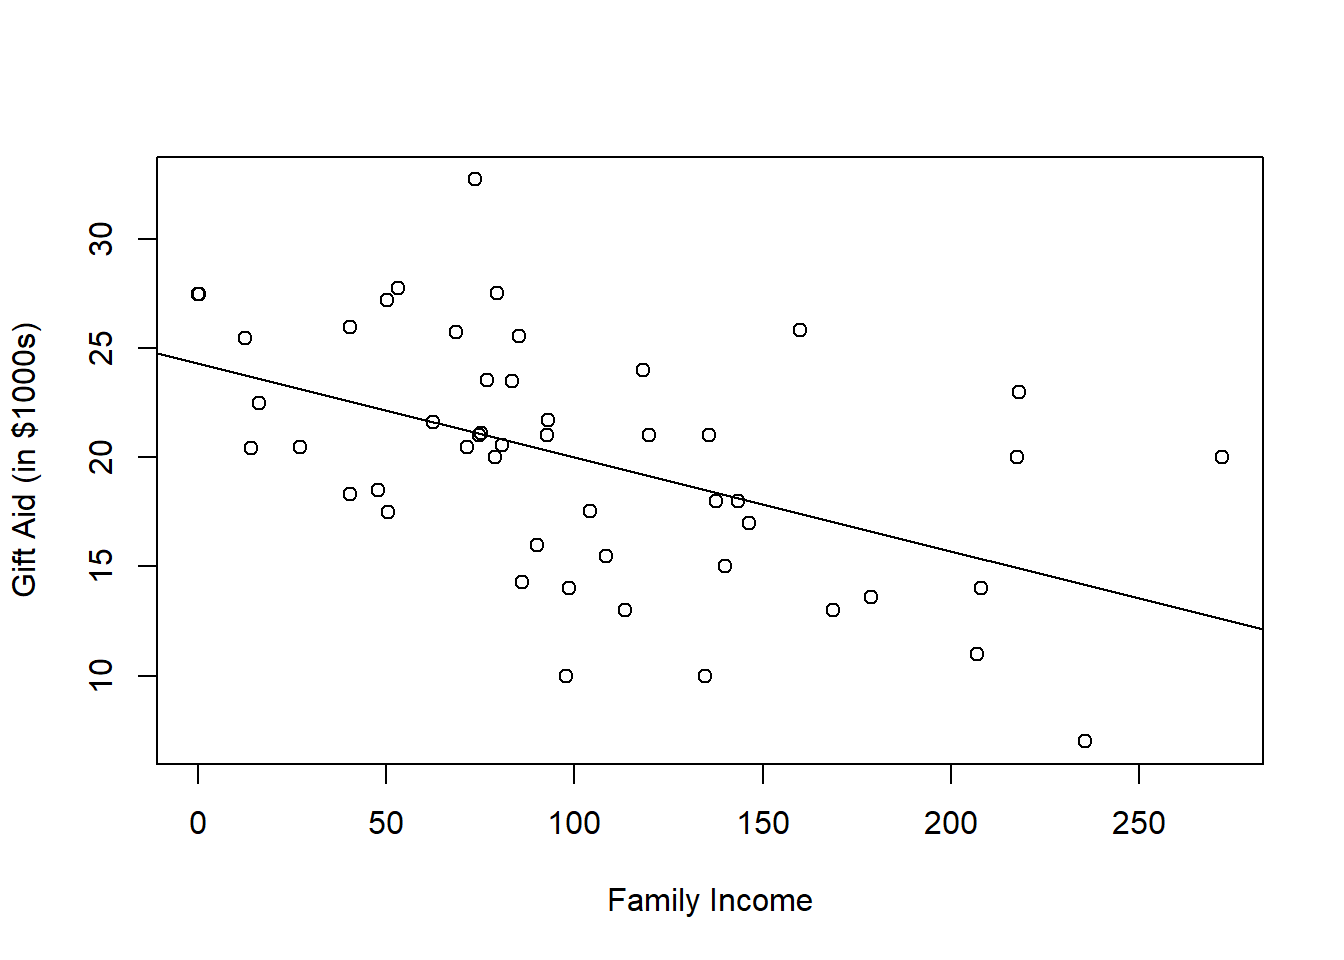
\includegraphics{bookdown-demo_files/figure-latex/elmhurst-1.pdf}
\caption{\label{fig:elmhurst}Scatterplot of Gift Aid Against Family Income}
\end{figure}

In Figure \ref{fig:elmhurst}, we see that the data points are evenly scattered around the fitted line. We also see the vertical variation of the data points is fairly constant. So assumptions that the errors have 0 mean and constant variance appear to be met.

\hypertarget{practice-question}{%
\subsubsection{Practice question}\label{practice-question}}

The data are about the prices of used cars. We are regressing the sale price of the car against the age of the car. The corresponding scatterplot is shown in Figure \ref{fig:mazda}. Based on Figure \ref{fig:mazda}, which of assumptions 1 or 2 (or both, or neither), is met? We will go over this in the tutorial.

\begin{figure}
\centering
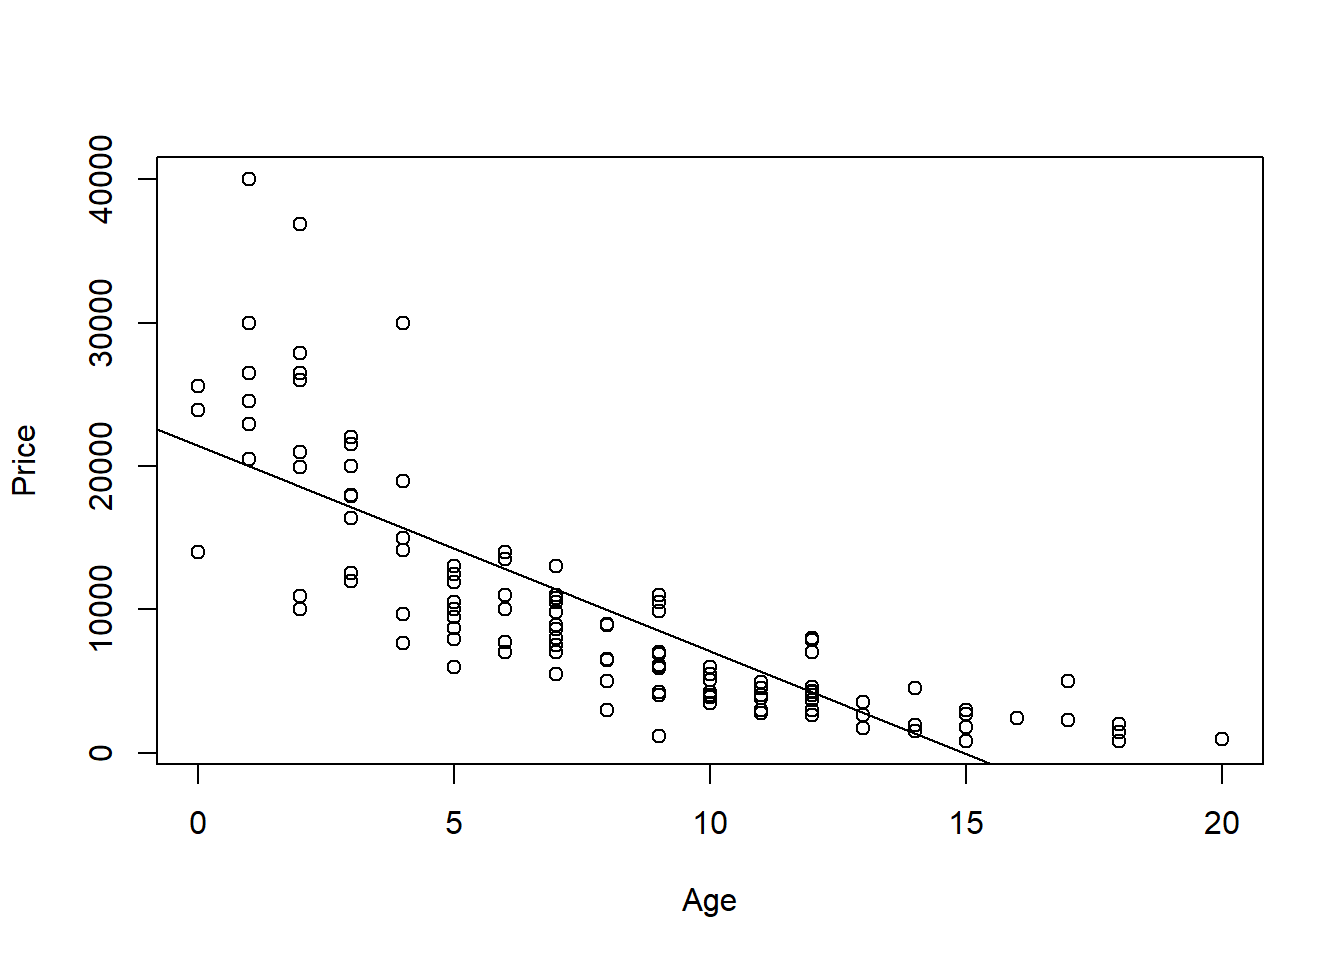
\includegraphics{bookdown-demo_files/figure-latex/mazda-1.pdf}
\caption{\label{fig:mazda}Scatterplot of Sale Price Against Age}
\end{figure}

\hypertarget{residual-plot}{%
\subsection{Residual plot}\label{residual-plot}}

While using the scatterplot is an intuitive way of assessing regression assumptions, it has a limitation. It cannot be used if we have multiple predictors in our regression, which we will encounter (and happens more often than just having one predictor). Another visualization that we can use to assess assumptions 1 and 2 is a \textbf{residual plot}. This is a scatterplot of residuals, \(e\), against fitted values, \(\hat{y}\). We want to observe the following in a residual plot.

\begin{itemize}
\tightlist
\item
  Residuals should be \textbf{evenly scattered} across the horizontal axis (assumption 1).
\item
  The residuals should have \textbf{similar vertical variation} across the plot (assumption 2).
\item
  Some writers combine these two points into the following statement: the residuals should fall in a \textbf{horizontal band around 0} with no apparent pattern (assumption 1, 2).
\end{itemize}

The residual plots in Figure are based on simulated data from Figures , , and .

We make the following observations:
- From Figure , we see that the residuals are evenly scattered across the horizontal axis, and their vertical variation is fairly constant across the plot. So both assumptions are met.
- From Figure , we see that the residuals are \textbf{not} evenly scattered across the horizontal axis, although their vertical variation is fairly constant across the plot. So only assumption 1 is not met.
- From Figure , we see that the residuals are evenly scattered across the horizontal axis, but their vertical variation is \textbf{not constant} across the plot. In fact, the vertical variation is increasing as we move from left to right. So only assumption 2 is not met.

If you compare the conclusions from the residuals plots and scatterplots, they are the same. In SLR, the takeaways should be consistent.

\emph{Please see the associated video for more explanation on how to use Figure to assess assumptions 1 and 2.}

\hypertarget{practice-questions-2}{%
\subsubsection{Practice questions}\label{practice-questions-2}}

\begin{enumerate}
\def\labelenumi{\arabic{enumi}.}
\tightlist
\item
  The residual plot in Figure \ref{fig:elmhurst-res} comes from regressing gift aid against family income for the \texttt{elmhurst} dataset. Based on this residual plot, which assumptions are met?
\end{enumerate}

\begin{figure}
\centering
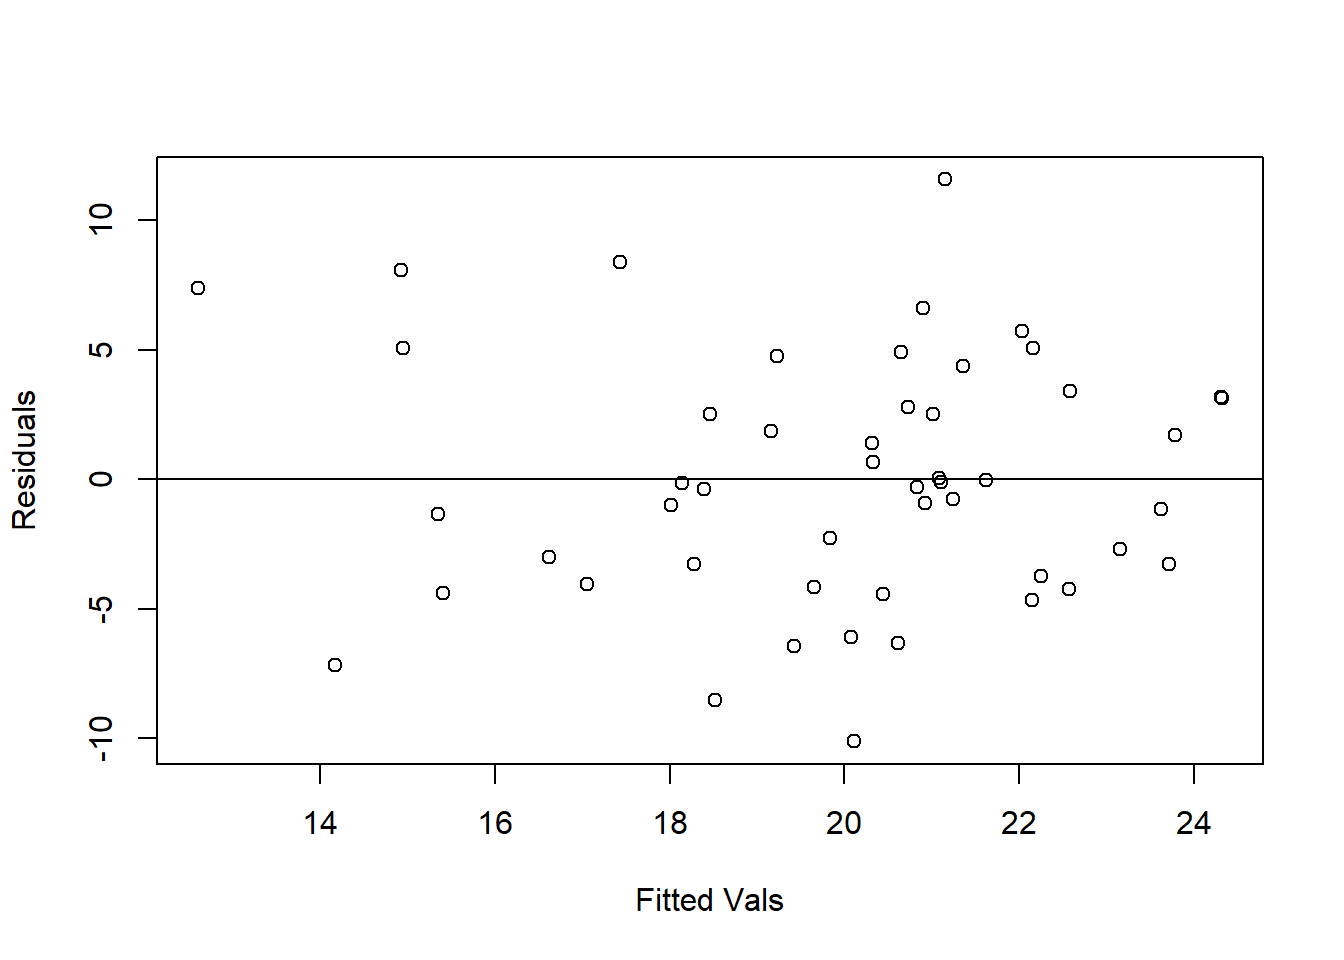
\includegraphics{bookdown-demo_files/figure-latex/elmhurst-res-1.pdf}
\caption{\label{fig:elmhurst-res}Residual Plot Regressing Gift Aid Against Family Income}
\end{figure}

\begin{enumerate}
\def\labelenumi{\arabic{enumi}.}
\setcounter{enumi}{1}
\tightlist
\item
  The residual plot in Figure \ref{fig:mazda-res} comes from regressing price of cars against age for the used cars dataset. Based on this residual plot, which assumptions are met?
\end{enumerate}

\begin{figure}
\centering
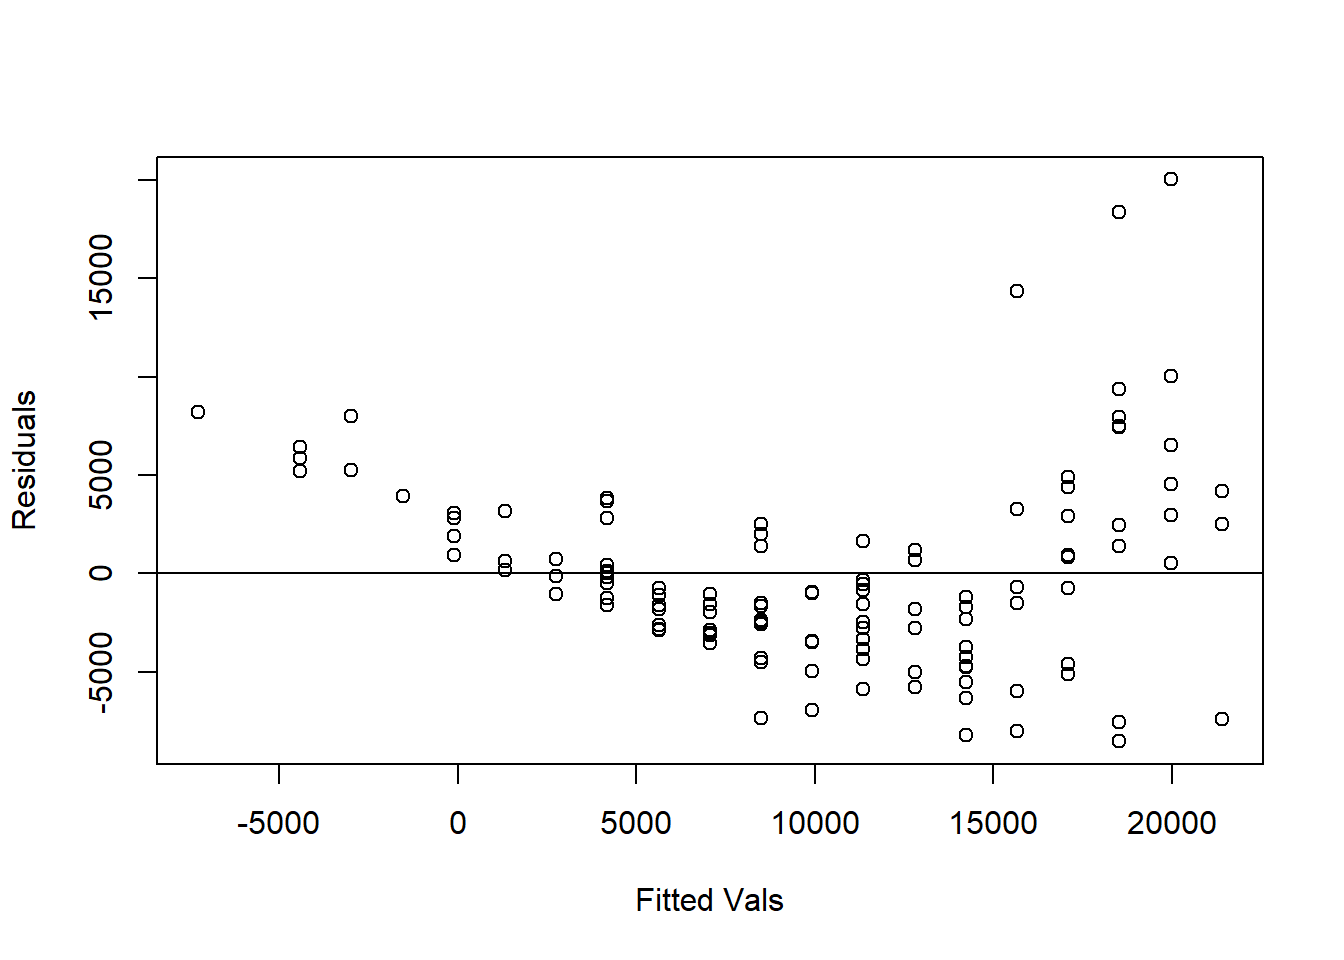
\includegraphics{bookdown-demo_files/figure-latex/mazda-res-1.pdf}
\caption{\label{fig:mazda-res}Residual Plot Regressing Price Against Age for Used Cars}
\end{figure}

\emph{Please see the associated video as I go over these practice questions.}

\hypertarget{acf-plot}{%
\subsection{ACF plot}\label{acf-plot}}

Assumption 3 states that the errors are \textbf{independent}. This assumption implies that the values of the response variable are independent from each other. This assumption is typically assessed via knowing the nature of the data.

\begin{itemize}
\item
  If the observations were obtained from a random sample, it is likely that the observations will be independent from each other. This is the very nature of a random sample and why random samples are preferred over convenience samples.
\item
  If the data has some inherent sequence, it is likely the observations will not be independent, and are dependent. For example, if I record the value of a stock at the end of each day, the value at day 2 is likely to be related to its value at day 1. So the values of stock prices at the end of each day are not independent.
\end{itemize}

An autocorrelation function (ACF) plot of the residuals may be a used to help assess if the assumption that the errors are independent is met. However, the plot is not a substitute for using your understanding about the nature of the data and should only be used as a confirmation.

The ACF plot measures the correlation between a vector of observations and the lagged versions of the observations. If the observations are uncorrelated, the correlations between the vector of observations and lagged versions of these observations are theoretically 0. We may create an ACF plot for the residuals from our regression.

The ACF plot in Figure and is based on simulated data that were independently generated.

A few notes about the ACF plot:

\begin{itemize}
\tightlist
\item
  The ACF at lag 0 is always 1. The correlation of any vector with itself is always 1.
\item
  The dashed horizontal lines represent critical values. An ACF at any lag beyond the critical value indicates an ACF that is significant. We have evidence of correlation (and hence dependence) in our residuals.
\item
  If the observed values for the response variable are independent, then we would expect the ACFs at lags greater than 0 to be insignificant. Do note that because we are conducting multiple hypothesis tests, do not be too alarmed if the ACFs are slightly beyond the critical values at an isolated lag or 2.
\end{itemize}

Based on Figure , we see that the ACFs at all lags greater than 0 are insignificant. We do not have evidence the residuals are correlated with each other, so we do not have evidence that assumption 3 is not met.

Sometimes, the dataframe can be sorted in some manner (e.g.~increasing order for response variable), and if so, we would actually expect to see significant correlations in the ACF plot. The ACF plot in Figure is such an example. The residuals are from the same simulated dataset, only with the data sorted by the response variable. If we had just looked at the ACF plot in Figure without understanding the data were simulated independently and then sorted, we would have erroneously concluded that the residuals are not independent and the regression assumption is not met.

\hypertarget{qq-plot}{%
\subsection{QQ plot}\label{qq-plot}}

A normal probability plot (also called a QQ plot) is used to assess if the distribution of a variable is normal. It typically plots the residuals against their theoretical residual if they followed a normal distribution. A QQ line is typically overlaid. If the plots fall closely to the QQ line, we have evidence that the observations follow a normal distribution. Figure \ref{fig:qq} shows a QQ plot that comes from a normally distributed variable.

\begin{figure}
\centering
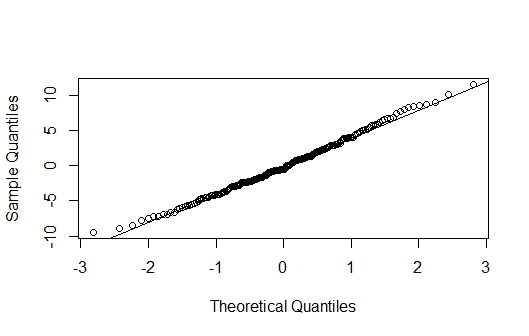
\includegraphics{images/qqplot.jpeg}
\caption{\label{fig:qq}QQ Plot}
\end{figure}

\hypertarget{remedial-measures}{%
\subsection{Remedial measures}\label{remedial-measures}}

We now know how to assess if specific regression assumptions are not met. The remedial measures involve transforming either the predictor variable and / or the response variable. These transformations are chosen to handle violations to assumptions 1 and / or 2 respectively. The general strategy on selecting which variable to transform:

\begin{itemize}
\tightlist
\item
  Transforming the response variable, \(y\), affects both assumptions 1 and 2.

  \begin{itemize}
  \tightlist
  \item
    Visually, we can think of transforming \(y\) in terms of stretching or squeezing the scatterplot of \(y\) against \(x\) vertically. Thus, transforming \(y\) affects the shape of the relationship and the vertical spread of the data points.
  \item
    However, the \textbf{choice on how we transform \(y\) is based on handling assumption 2.}
  \end{itemize}
\item
  Transforming the predictor variable, \(x\) affects assumption 1 and does not theoretically affect assumption 2.

  \begin{itemize}
  \tightlist
  \item
    Visually, we can think of transforming \(x\) in terms of stretching or squeezing the scatterplot of \(y\) against \(x\) horizontally. Thus, transforming \(x\) affects the shape of the relationship but not the vertical spread of the data points.
  \item
    Therefore, \textbf{transforming \(x\) is based on handling assumption 1.}
  \end{itemize}
\item
  If assumption 2 is not met, we transform \(y\) to stabilize the variance and make it constant.
\item
  If assumption 1 is not met, we transform \(x\) to find the appropriate shape to relate the variables.
\item
  If both assumptions are not met, we transform \(y\) first to stabilize the variance. Once assumption 2 is solved, check if assumption 1 is not met. If not met, transform \(x\).
\end{itemize}

Assumption 1 deals with whether the way we have expressed how \(y\) and \(x\) are related, through \(f(x)\), is appropriate. Assumption 2 deals with the vertical variation of the data points in the scatterplot.

\hypertarget{remedial-measures-variance-stabilizing-transformations}{%
\section{Remedial Measures: Variance Stabilizing Transformations}\label{remedial-measures-variance-stabilizing-transformations}}

We transform the response variable to stabilize the variance (assumption 2). There are a couple of ways to decide the appropriate transformation:

\begin{enumerate}
\def\labelenumi{\arabic{enumi}.}
\tightlist
\item
  Pattern seen in residual plot can guide choice in how to transform the response variable.
\item
  Box-Cox plot.
\end{enumerate}

\hypertarget{use-pattern-in-residual-plot}{%
\subsection{Use Pattern in Residual Plot}\label{use-pattern-in-residual-plot}}

We can stabilize the variance of the errors based on the residual plot, if we see either of the following scenarios:

\begin{itemize}
\tightlist
\item
  vertical variation of residuals \textbf{increasing} as fitted response increases, or as we move from left to right, as in Figure , or
\item
  vertical variation of residuals \textbf{decreasing} as fitted response increases, or as we move from left to right, as in Figure .
\end{itemize}

Note that increasing variance as fitted response increases is much more common with real data. Generally, larger values of a variable are associated with larger spread.

We transform \(y\) using \(y^{*} = y^{\lambda}\), with \(\lambda\) chosen based on whether the variance of the residuals is increasing or decreasing with fitted response:

\begin{itemize}
\tightlist
\item
  For Figure , choose \(\lambda < 1\).

  \begin{itemize}
  \tightlist
  \item
    If \(\lambda = 0\), it means we use a logarithmic transformation with base e, i.e.~\(y^* = \log(y)\).
  \item
    Note that a logarithm with no base means a natural log, or ln.
  \end{itemize}
\item
  For Figure , choose \(\lambda > 1\).
\end{itemize}

So based on the residual plot, we have a range of values for \(\lambda\).

\hypertarget{box-cox-plot}{%
\subsection{Box-Cox Plot}\label{box-cox-plot}}

We can use a Box-Cox plot to help us narrow the range of \(\lambda\) to use. It is a plot of the log-likelihood function against \(\lambda\), and we choose \(\lambda\) that maximizes this log-likelihood function. For example, Figure shows the Box Cox plot generated for the regression associated with the residual plot in Figure .

Notice an approximate 95\% CI is provided for \(\lambda\). A few comments on how to use the Box-Cox plot:

\begin{itemize}
\tightlist
\item
  Three vertical dashed lines are displayed: the middle line corresponds to the optimal value of \(\lambda\); the other two lines are the lower and upper bounds of a 95\% CI for \(\lambda\).
\item
  We choose \(\lambda\) within the CI (or even close to it) that is easy to understand. We do not have to choose the optimal value, especially if its value is difficult to interpret. In this example, I will choose \(\lambda = 2\), so a square transformation for \(y\). Transform response with \(y^* = y^2\). Regress \(y^*\) against \(x\).
\item
  If 1 lies in the CI, \textbf{no transformation} on \(y\) may be needed.
\item
  If a transformation is needed, a \textbf{log transformation} is preferred, since we can still interpret the estimated coefficients. It is difficult to interpret with any other type of transformation.
\item
  View the Box-Cox procedure as a guide for selecting a transformation, rather than being definitive.
\item
  Need to recheck the residuals after every transformation to assess if the transformation worked.
\end{itemize}

\hypertarget{interpretation-with-log-transformed-response}{%
\subsection{Interpretation with Log Transformed Response}\label{interpretation-with-log-transformed-response}}

A log transformation on the response is preferred over any other transformation, as we can still interpret regression coefficients. A couple of ways to interpret the estimated slope \(\hat{\beta}_1\):

\begin{itemize}
\tightlist
\item
  The predicted response variable is \textbf{multiplied by a factor} of \(\exp(\hat{\beta_1})\) for a one-unit increase in the predictor.
\item
  We can also subtract 1 from \(\exp(\hat{\beta_1})\) to express the change as a percentage.

  \begin{itemize}
  \tightlist
  \item
    If \(\hat{\beta}_1\) is positive, we have a percent \textbf{increase}. The predicted response variable increases by \((\exp(\hat{\beta_1}) - 1) \times 100\) percent for a one-unit increase in the predictor.
  \item
    If \(\hat{\beta}_1\) is negative, we have a percent \textbf{decrease}. The predicted response variable decreases by \((1 - \exp(\hat{\beta_1})) \times 100\) percent for a one-unit increase in the predictor.
  \end{itemize}
\end{itemize}

\emph{Please see the associated video as I go over the math explaining how we interpret regression coefficients when the response variable is log transformed.}

\hypertarget{remedial-measures-linearization-transformations}{%
\section{Remedial Measures: Linearization Transformations}\label{remedial-measures-linearization-transformations}}

We first ensure the variance has been stabilized and assumption 2 is met. If \(f(x)\) does not accurately capture the relationship between the variables, we transform the predictor variable to meet assumption 1. Some writers call this a linearization transformation, as we seek to make the transformed version of the predictor variable, \(x^*\), to be approximately linear with the response variable (or transformed \(y\)), i.e.~\(y = \beta_0 + \beta_1 x^* + \epsilon\). We do not consider transforming the response variable to deal with assumption 1, as transforming the response variable is likely to reintroduce violation of assumption 2.

The general strategy on how to transform the predictor is via a scatterplot of \(y\) (or \(y^*\)) against \(x\). We use the pattern seen in the plot to decide how to transform the predictor. Some examples are shown in Figure below.

\hypertarget{hierarchical-principle}{%
\subsection{Hierarchical Principle}\label{hierarchical-principle}}

One thing to be aware of is the \textbf{hierarchical principle}: if the relationship between the response and predictor is of a higher order polynomial (e.g.~quadratic, cubic), the hierarchical principle states that the lower order terms should remain in the model. For example, if the relationship is of order \(h\), fit \(y = \beta_0 + \beta_1 x + \beta_2 x^2 + \cdots + \beta_h x^h + \epsilon\) via a multiple linear regression framework. We will see how to do this in the next module.

\hypertarget{interpretation-with-log-transformed-predictor}{%
\subsection{Interpretation with Log Transformed Predictor}\label{interpretation-with-log-transformed-predictor}}

A log transformation on the predictor is preferred over any other transformation, as we can still interpret the regression coefficient, \(\hat{\beta}_1\), in a couple of ways:

\begin{itemize}
\tightlist
\item
  For an \(a\%\) increase in the predictor, the predicted response \textbf{increases by \(\hat{\beta}_1 \log(1+ \frac{a}{100})\).}
\item
  \(\log(1 + \frac{1}{100}) \approx \frac{1}{100}\) (Taylor series). So an alternative interpretation is: for a 1\% increase in the predictor, the predicted response increases by approximately \(\frac{\hat{\beta}_1}{100}\).
\end{itemize}

\emph{Please see the associated video as I go over the math explaining how we interpret regression coefficients when the predictor variable is log transformed.}

\hypertarget{interpretation-with-log-transformed-response-and-predictor}{%
\subsection{Interpretation with Log Transformed Response and Predictor}\label{interpretation-with-log-transformed-response-and-predictor}}

If both response and predictor variables are log transformed, the regression coefficient, \(\hat{\beta}_1\), can be interpreted in a couple of ways:

\begin{itemize}
\item
  For an \(a\%\) increase in the predictor, the predicted response is \textbf{multiplied by \((1 + \frac{a}{100})^{\hat{\beta}_1}\).}
\item
  \((1 + \frac{1}{100})^{\hat{\beta}_1} \approx 1 + \frac{\hat{\beta}_1}{100}\) (Taylor series). So an alternative interpretation is: for a 1\% increase in the predictor, the predicted response \textbf{increases by approximately \(\hat{\beta}_1\) percent.} Note that this approximation works better when \({\hat{\beta}_1}\) is small in magnitude.
\end{itemize}

\emph{Please see the associated video as I go over the math explaining how we interpret regression coefficients when the both response and predictor variables are log transformed.}

\hypertarget{some-general-comments-about-assessing-assumptions-and-transformations}{%
\subsection{Some General Comments about Assessing Assumptions and Transformations}\label{some-general-comments-about-assessing-assumptions-and-transformations}}

\begin{itemize}
\item
  When assessing the assumptions with a residual plot, we are assessing if the assumptions are reasonably / approximately met.
\item
  With real data, assumptions are rarely met 100\%.
\item
  If unsure, proceed with model building, and test how model performs on new data. If poor performance, go back to residual plot to assess what transformation will be appropriate.
\item
  Assess the plots to decide which variables need to be transformed, and how. The choice of transformation should be guided by what you see in the plots, and not by trial and error.
\item
  A residual plot should always be produced after each transformation. A Box Cox plot could also be produced. The plots should be assessed if the transformation helped in the way you intended.
\item
  Solve assumption 2 first, then assumption 1.
\end{itemize}

\hypertarget{try}{%
\chapter{TABLE}\label{try}}

\hypertarget{introduction-5}{%
\section{Introduction}\label{introduction-5}}

\begin{longtable}[]{@{}
  >{\centering\arraybackslash}p{(\columnwidth - 8\tabcolsep) * \real{0.2353}}
  >{\centering\arraybackslash}p{(\columnwidth - 8\tabcolsep) * \real{0.2941}}
  >{\centering\arraybackslash}p{(\columnwidth - 8\tabcolsep) * \real{0.1569}}
  >{\centering\arraybackslash}p{(\columnwidth - 8\tabcolsep) * \real{0.1569}}
  >{\centering\arraybackslash}p{(\columnwidth - 8\tabcolsep) * \real{0.1569}}@{}}
\toprule\noalign{}
\begin{minipage}[b]{\linewidth}\centering
Source of Variation
\end{minipage} & \begin{minipage}[b]{\linewidth}\centering
SS
\end{minipage} & \begin{minipage}[b]{\linewidth}\centering
df
\end{minipage} & \begin{minipage}[b]{\linewidth}\centering
MS
\end{minipage} & \begin{minipage}[b]{\linewidth}\centering
F
\end{minipage} \\
\midrule\noalign{}
\endhead
\bottomrule\noalign{}
\endlastfoot
Regression & \(SS_R=\sum\left(\hat{y_i}-\bar{y}\right)^2\) & \(df_R = 1\) & \(MS_R=\frac{SS_R}{df_R}\) & \(\frac{MS_R}{MS_{res}}\) \\
Error & \(SS_{res} = \sum\left(y_i-\hat{y_i}\right)^2\) & \(df_{res} = n-2\) & \(MS_{res}=\frac{SS_{res}}{df_{res}}\) & \texttt{***} \\
Total & \(SS_T=\sum\left(y_i-\bar{y}\right)^2\) & \(df_T = n-1\) & \texttt{***} & \texttt{***} \\
\end{longtable}

\hypertarget{intro}{%
\chapter{Introduction}\label{intro}}

You can label chapter and section titles using \texttt{\{\#label\}} after them, e.g., we can reference Chapter \ref{intro}. If you do not manually label them, there will be automatic labels anyway, e.g., Chapter \ref{methods}.

Figures and tables with captions will be placed in \texttt{figure} and \texttt{table} environments, respectively.

\begin{Shaded}
\begin{Highlighting}[]
\FunctionTok{par}\NormalTok{(}\AttributeTok{mar =} \FunctionTok{c}\NormalTok{(}\DecValTok{4}\NormalTok{, }\DecValTok{4}\NormalTok{, .}\DecValTok{1}\NormalTok{, .}\DecValTok{1}\NormalTok{))}
\FunctionTok{plot}\NormalTok{(pressure, }\AttributeTok{type =} \StringTok{\textquotesingle{}b\textquotesingle{}}\NormalTok{, }\AttributeTok{pch =} \DecValTok{19}\NormalTok{)}
\end{Highlighting}
\end{Shaded}

\begin{figure}

{\centering 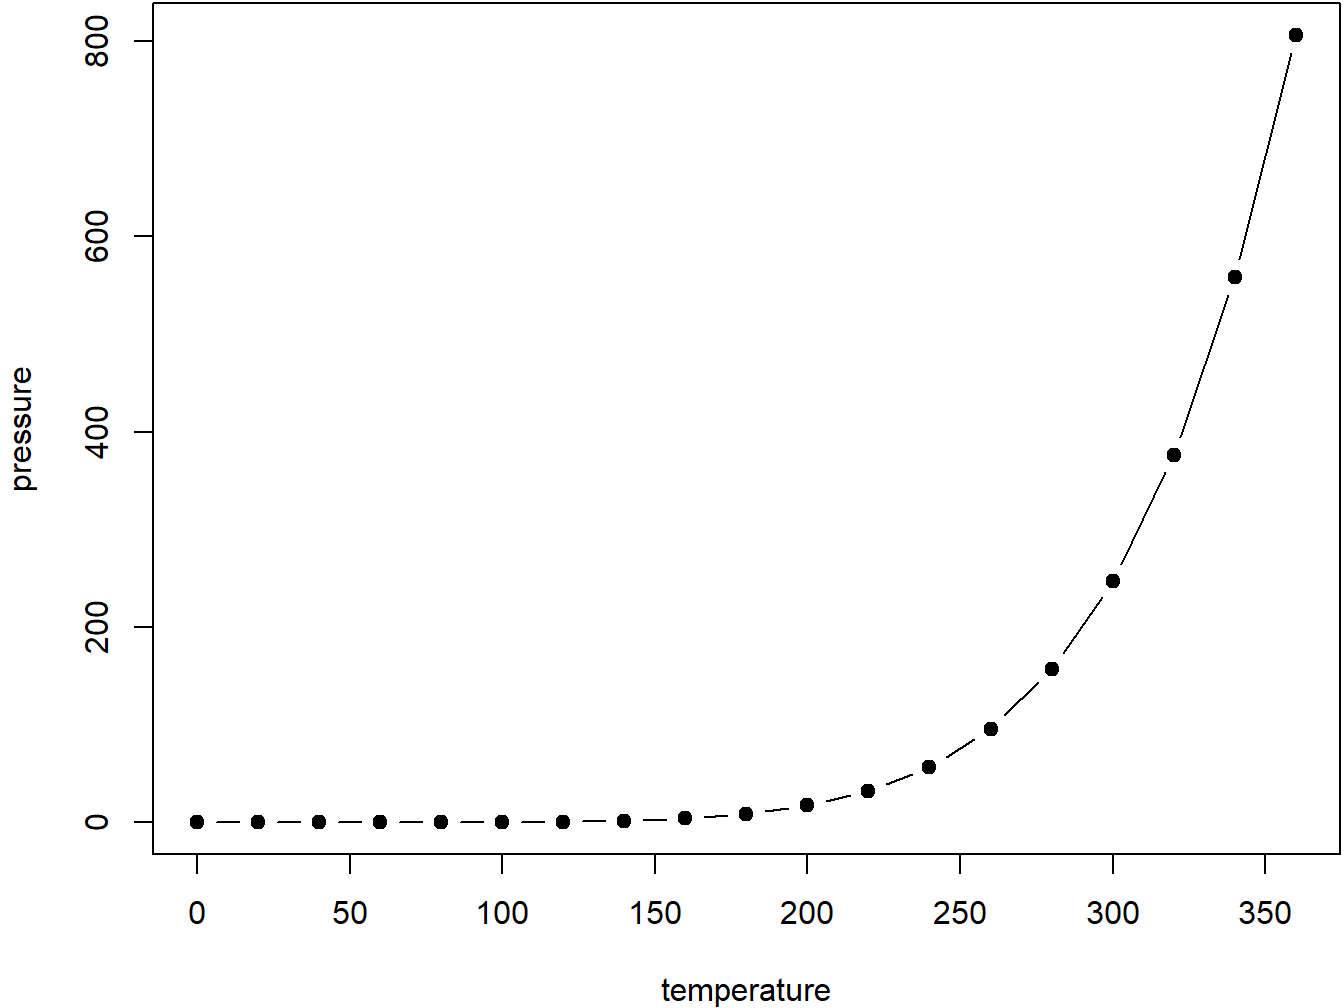
\includegraphics[width=0.8\linewidth]{bookdown-demo_files/figure-latex/nice-fig-1} 

}

\caption{Here is a nice figure!}\label{fig:nice-fig}
\end{figure}

Reference a figure by its code chunk label with the \texttt{fig:} prefix, e.g., see Figure \ref{fig:nice-fig}. Similarly, you can reference tables generated from \texttt{knitr::kable()}, e.g., see Table \ref{tab:nice-tab}.

\begin{Shaded}
\begin{Highlighting}[]
\NormalTok{knitr}\SpecialCharTok{::}\FunctionTok{kable}\NormalTok{(}
  \FunctionTok{head}\NormalTok{(iris, }\DecValTok{20}\NormalTok{), }\AttributeTok{caption =} \StringTok{\textquotesingle{}Here is a nice table!\textquotesingle{}}\NormalTok{,}
  \AttributeTok{booktabs =} \ConstantTok{TRUE}
\NormalTok{)}
\end{Highlighting}
\end{Shaded}

\begin{table}

\caption{\label{tab:nice-tab}Here is a nice table!}
\centering
\begin{tabular}[t]{rrrrl}
\toprule
Sepal.Length & Sepal.Width & Petal.Length & Petal.Width & Species\\
\midrule
5.1 & 3.5 & 1.4 & 0.2 & setosa\\
4.9 & 3.0 & 1.4 & 0.2 & setosa\\
4.7 & 3.2 & 1.3 & 0.2 & setosa\\
4.6 & 3.1 & 1.5 & 0.2 & setosa\\
5.0 & 3.6 & 1.4 & 0.2 & setosa\\
\addlinespace
5.4 & 3.9 & 1.7 & 0.4 & setosa\\
4.6 & 3.4 & 1.4 & 0.3 & setosa\\
5.0 & 3.4 & 1.5 & 0.2 & setosa\\
4.4 & 2.9 & 1.4 & 0.2 & setosa\\
4.9 & 3.1 & 1.5 & 0.1 & setosa\\
\addlinespace
5.4 & 3.7 & 1.5 & 0.2 & setosa\\
4.8 & 3.4 & 1.6 & 0.2 & setosa\\
4.8 & 3.0 & 1.4 & 0.1 & setosa\\
4.3 & 3.0 & 1.1 & 0.1 & setosa\\
5.8 & 4.0 & 1.2 & 0.2 & setosa\\
\addlinespace
5.7 & 4.4 & 1.5 & 0.4 & setosa\\
5.4 & 3.9 & 1.3 & 0.4 & setosa\\
5.1 & 3.5 & 1.4 & 0.3 & setosa\\
5.7 & 3.8 & 1.7 & 0.3 & setosa\\
5.1 & 3.8 & 1.5 & 0.3 & setosa\\
\bottomrule
\end{tabular}
\end{table}

You can write citations, too. For example, we are using the \textbf{bookdown} package \citep{R-bookdown} in this sample book, which was built on top of R Markdown and \textbf{knitr} \citep{xie2015}.

\hypertarget{literature}{%
\chapter{Literature}\label{literature}}

Here is a review of existing methods.

\hypertarget{new-section}{%
\section{New section}\label{new-section}}

Add some text here. BLAH BLAH

\hypertarget{methods}{%
\chapter{Methods}\label{methods}}

We describe our methods in this chapter.

Math can be added in body using usual syntax like this

\hypertarget{math-example}{%
\section{math example}\label{math-example}}

\(p\) is unknown but expected to be around 1/3. Standard error will be approximated

\[
SE = \sqrt(\frac{p(1-p)}{n}) \approx \sqrt{\frac{1/3 (1 - 1/3)} {300}} = 0.027
\]

You can also use math in footnotes like this\footnote{where we mention \(p = \frac{a}{b}\)}.

We will approximate standard error to 0.027\footnote{\(p\) is unknown but expected to be around 1/3. Standard error will be approximated

  \[
  SE = \sqrt(\frac{p(1-p)}{n}) \approx \sqrt{\frac{1/3 (1 - 1/3)} {300}} = 0.027
  \]}

\hypertarget{applications}{%
\chapter{Applications}\label{applications}}

Some \emph{significant} applications are demonstrated in this chapter.

\hypertarget{example-one}{%
\section{Example one}\label{example-one}}

\hypertarget{example-two}{%
\section{Example two}\label{example-two}}

\hypertarget{final-words}{%
\chapter{Final Words}\label{final-words}}

We have finished a nice book.

  \bibliography{book.bib,packages.bib}

\end{document}
